\documentclass[12pt,a4paper,titlepage]{book}
\usepackage[a4paper]{geometry}

%\documentclass[ebook,11pt,oneside,openany]{memoir}
\usepackage[english]{babel}
\usepackage{CJKutf8} 
\usepackage{mathtools}
\usepackage{graphicx}
\usepackage{subfig}
 \usepackage{fancybox}
\usepackage{framed}
\usepackage{lipsum}
\usepackage{color}
\usepackage{wrapfig}
\usepackage{amsfonts}
\usepackage{amsmath}
\usepackage{amssymb}
\usepackage{stmaryrd}
\usepackage{tikz}
\usepackage[boxed,linesnumbered,algochapter]{algorithm2e}  

\graphicspath{{figures/}} 
\newcommand*{\vv}[1]{\vec{\mkern0mu#1}}
\renewcommand{\baselinestretch}{1.5} 
\title{机器学习中的那些证明}
\author{Shujie Liu (j4ckl1u@gmail.com)}

\begin{document}
\begin{CJK*}{UTF8}{gbsn} 
\maketitle
% !Mode:: "TeX:UTF-8"

\chapter{概率分布}
\section{Gamma 函数和Gamma 分布}
Gamma函数的定义为:
\begin{displaymath}
\begin{split}
\Gamma(x)=\int_{0}^{\infty}{u^{x-1}e^{-u}du}
\end{split}
\end{displaymath}
Gama函数的性质:
$\Gamma(1)=1; \Gamma(x+1)=x\Gamma(x); \Gamma(x+1) = x!; \Gamma(\frac{1}{2}) = \sqrt{\pi}$
其中, $\alpha$为形状参数,而$\beta$为尺度参数。

Gamma分布:
\begin{displaymath}
\begin{split}
Gamma(x) = \frac{x^{(\alpha-1)} \lambda^\alpha e^{(-\lambda x)}}{\Gamma(\alpha)}, x > 0
\end{split}
\end{displaymath}

\begin{figure}[htbp]
\centering
\begin{subfloat}
\centering
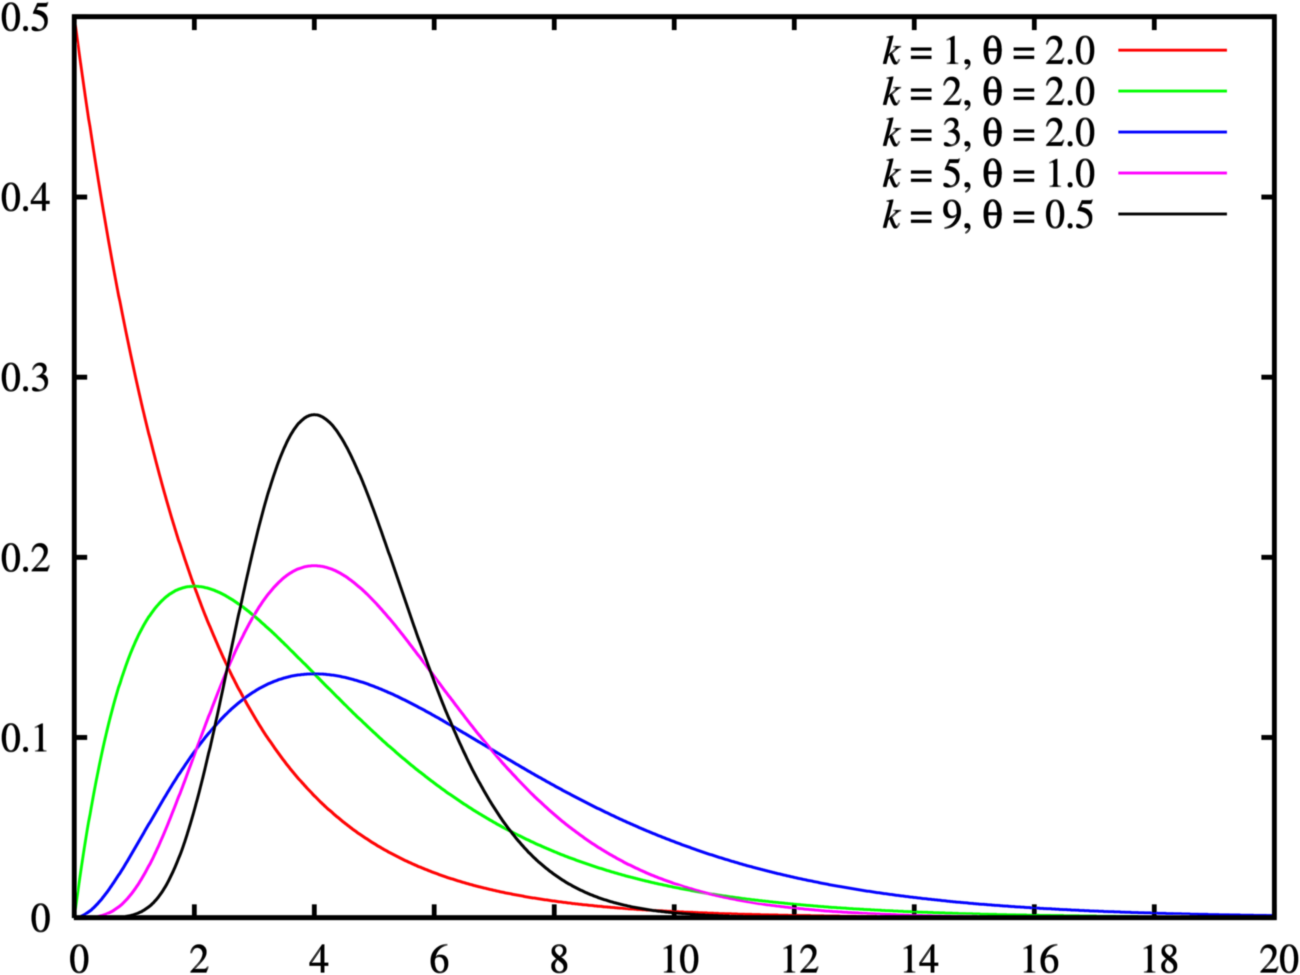
\includegraphics[width = 0.4\textwidth]{figures/Gamma_distribution_pdf.jpg}
\end{subfloat}
\begin{subfloat}
\centering
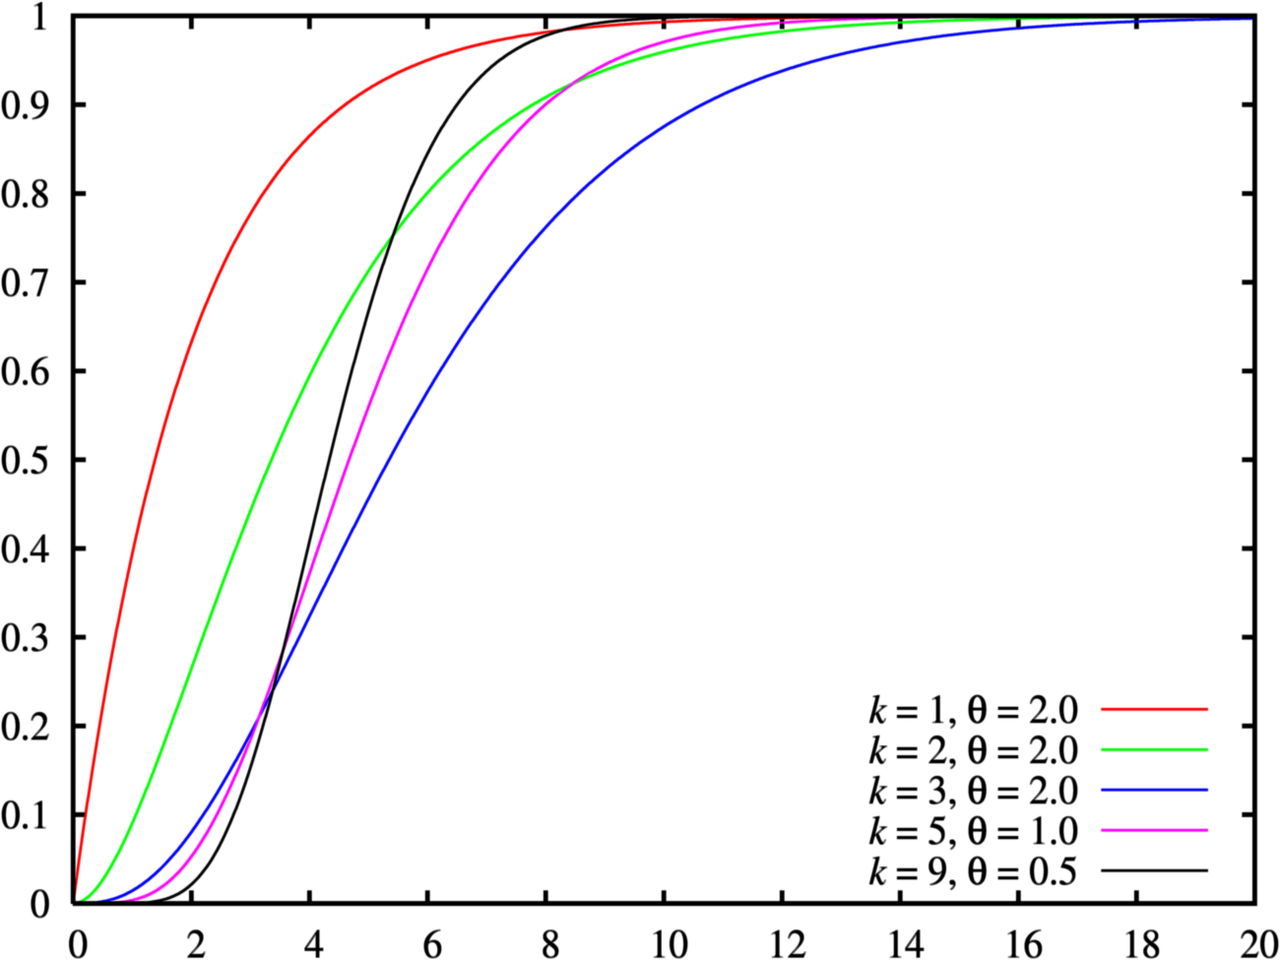
\includegraphics[width = 0.4\textwidth]{figures/Gamma_distribution_cdf.jpg}
\end{subfloat}
\caption{Gamma Distribution}
\end{figure}

参考《Numerical Recipes》第7章,我们有从Gamma分布采样的算法如下:

\begin{minipage}{0.8\textwidth}\centering
\begin{algorithm}[H]
\textbf{Sample from Gamma Distribution}($x \sim Gamma(\alpha, \beta)$):\\
\If{$\alpha < 1$}{
sample $u \sim U(0,1)$;\\
sample $g \sim Gamma(1+\alpha, \beta)$;\\
return $gu^{\frac{1}{\alpha}}$;\\
}
$d=\alpha - \frac{1}{3}, c=\frac{1}{\sqrt{9d}}$;\\
\While{true}{
$v=-1$;\\
\While{$v <= 0$}
{
sample $x \sim N(0,1)$;\\
$v=1+cx$;\\
}
$v = v^3$;\\
sample $u \sim U(0,1)$;\\
\If{$u < 1-0.331x^4$}{
return $\frac{dv}{\beta}$;\\
}
\If{$\ln{u} < 0.5x^2 + d(1-v+\ln{v})$}{
return $\frac{dv}{\beta}$;\\
}

}
\end{algorithm}
\end{minipage}

\begin{figure}[htbp]
\centering
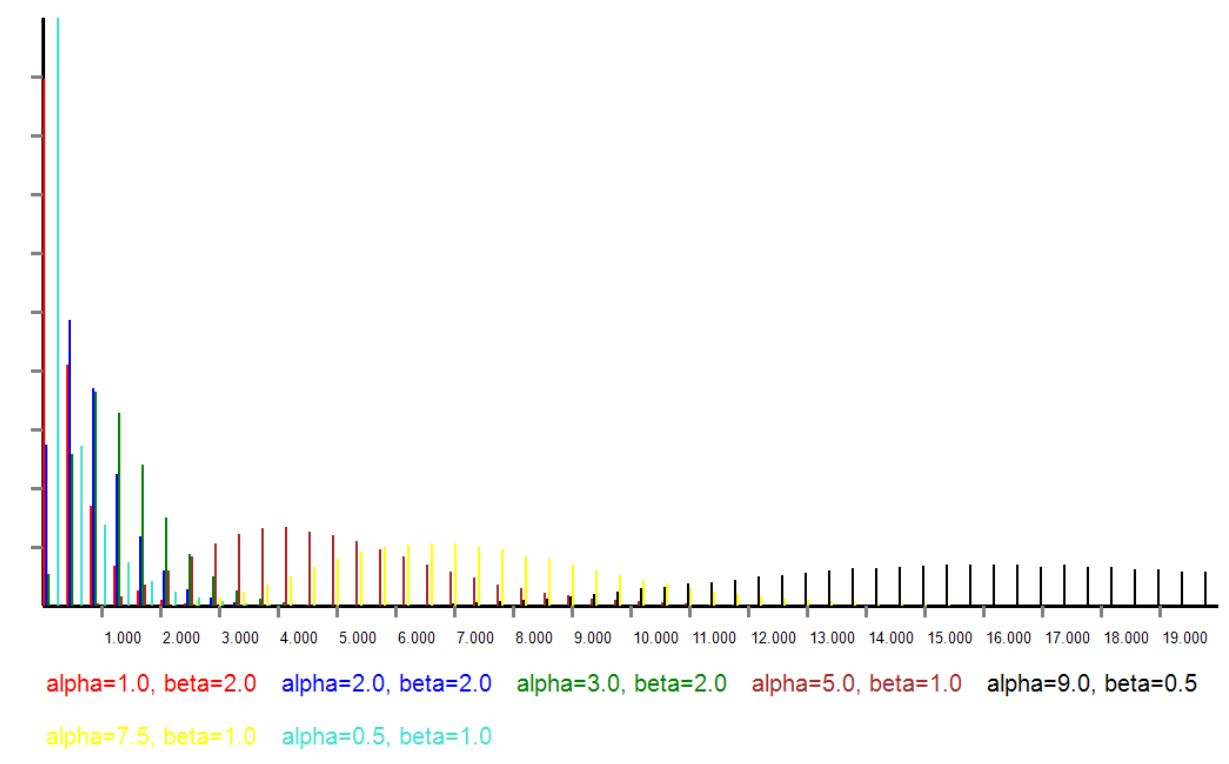
\includegraphics[width = 0.9\textwidth]{GammaDistributionSample}
\caption{从Gamma分布中进行采样}
\end{figure}

\section{Beta-Binomial共轭}

\begin{displaymath}
\begin{split}
Beta(\mu|a,b) &= \frac{\Gamma(a+b)}{\Gamma(a)\Gamma(b)} \mu^{a-1} (1-\mu)^{b-1}\\
Bin(k|\mu, n)  &= \frac{n!}{k!(n-k)!} \mu^k(1-\mu)^{n-k}\\
\end{split}
\end{displaymath}

\begin{displaymath}
\begin{split}
p(\mu|n,k,a,b) &=\frac{Beta(\mu|a,b)Bin(k|\mu,n)}{p(k|n,a,b)}\\
&=\frac{
 \frac{\Gamma(a+b)}{\Gamma(a)\Gamma(b)} \mu^{a-1} (1-\mu)^{b-1} \frac{n!}{k!(n-k)!} \mu^k(1-\mu)^{n-k}
}{
\int_\mu \frac{\Gamma(a+b)}{\Gamma(a)\Gamma(b)} \mu^{a-1} (1-\mu)^{b-1} \frac{n!}{k!(n-k)!} \mu^k(1-\mu)^{n-k} \mathrm{d} \mu
} \\
&= \frac{
 \frac{(a+b-1)! n!}{(a-1)!(b-1)!k!(n-k)!} \mu^{k+a-1} (1-\mu)^{n-k+b-1}
}{
\int_\mu  \frac{(a+b-1)! n!}{(a-1)!(b-1)!k!(n-k)!} \mu^{k+a-1} (1-\mu)^{n-k+b-1} \mathrm{d} \mu
}\\
&= \frac{
 \mu^{k+a-1} (1-\mu)^{n-k+b-1}
}{
\int_0^1 \mu^{k+a-1} (1-\mu)^{n-k+b-1} \mathrm{d} \mu
}\\
&= \frac{
 \mu^{k+a-1} (1-\mu)^{n-k+b-1}
}{
\frac{\Gamma{(k+a)}\Gamma{(n+b-k)}}{\Gamma{(n+a+b)}}
}\\
&= Beta(\mu|a+k, b+n-k)\\
\end{split}
\end{displaymath}
其中:
\begin{displaymath}
\begin{split}
f(0,n) &= \frac{1}{n+1}\\
f(k,n) &= \int_0^1 p^{k}(1-p)^{n-k} \mathrm{d} p\\
&= -p^{k}\frac{(1-p)^{n-(k-1)}}{n-(k-1)} \Bigg |_0^1 + \int_0^1 kp^{k-1} \frac{(1-p)^{n-(k-1)}}{n-(k-1)} \mathrm{d} p\\
& =\int_0^1 kp^{k-1} \frac{(1-p)^{n-(k-1)}}{n-(k-1)} \mathrm{d} p\\
&= \frac{k}{n-(k-1)} \int_0^1 p^{k-1} {(1-p)^{n-(k-1)}} \mathrm{d} p\\
&= \frac{k}{n-(k-1)} f(k-1,n)\\
&= \frac{k(k-1)}{(n-(k-1))(n-(k-2))} f(k-2,n)\\
&= \frac{k(k-1)...1}{(n-(k-1))(n-(k-2))...n} f(0,n)\\
&= \frac{k(k-1)...1}{(n-(k-1))(n-(k-2))...n(n+1)}\\
&= \frac{k!}{\frac{(n+1)!}{(n-k)!}}\\
&= \frac{k!(n-k)!}{(n+1)!}\\
&= \frac{\Gamma(k+1)\Gamma(n-k+1)} {\Gamma(n+2)}\\
\end{split}
\end{displaymath}
另一种证明:
\begin{displaymath}
\begin{split}
&\int_0^1 \frac{\Gamma(n+2)}{\Gamma(k+1)\Gamma(n-k+1)} p^{k}(1-p)^{n-k} \mathrm{d} p = 1\\
\to & \frac{\Gamma(n+2)}{\Gamma(k+1)\Gamma(n-k+1)}  \int_0^1  p^{k}(1-p)^{n-k} \mathrm{d} p = 1\\
\to & \int_0^1  p^{k}(1-p)^{n-k} \mathrm{d} p =  \frac{\Gamma(k+1)\Gamma(n-k+1)} {\Gamma(n+2)} \\
\end{split}
\end{displaymath}
由此:
\begin{displaymath}
\begin{split}
\int_0^1 \mu^{k+a-1} (1-\mu)^{n-k+b-1} \mathrm{d} \mu 
&= \int_0^1 \mu^{k+a-1} (1-\mu)^{(n+a+b-2)-(k+a-1)} \mathrm{d} \mu \\
&= \frac{(k+a-1)!(n+b-k-1)!}{(n+a+b-1)!}\\
&= \frac{\Gamma{(k+a)}\Gamma{(n+b-k)}}{\Gamma{(n+a+b)}}
\end{split}
\end{displaymath}

\begin{figure}[htbp]
\centering
\begin{subfloat}
\centering
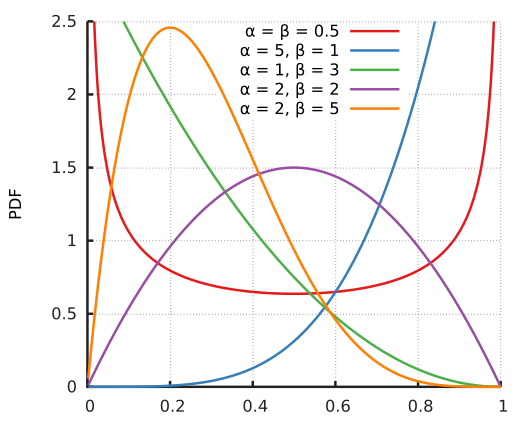
\includegraphics[width = 0.4\textwidth]{Beta_distribution_pdf}
\end{subfloat}
\begin{subfloat}
\centering
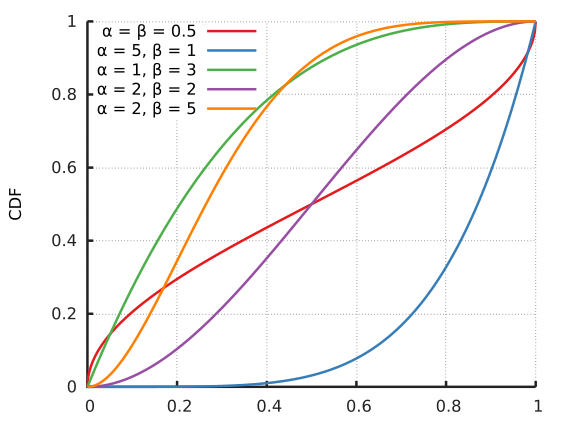
\includegraphics[width = 0.4\textwidth]{Beta_distribution_cdf}
\end{subfloat}
\caption{Beta Distribution}
\end{figure}

使用Gamma分布进行Beta分布采样的算法为:

\begin{minipage}{0.8\textwidth}\centering
\begin{algorithm}[H]
\textbf{Sample from Beta Distribution}($x \sim Beta(\alpha, \beta)$):\\
sample $x_0 \sim Gammma(\alpha, 1)$;\\
sample $x_1 \sim Gamma(\beta, 1)$;\\
return $\frac{x_0}{x_0+x_1}$;\\
\end{algorithm}
\end{minipage}

\begin{figure}[htbp]
\centering
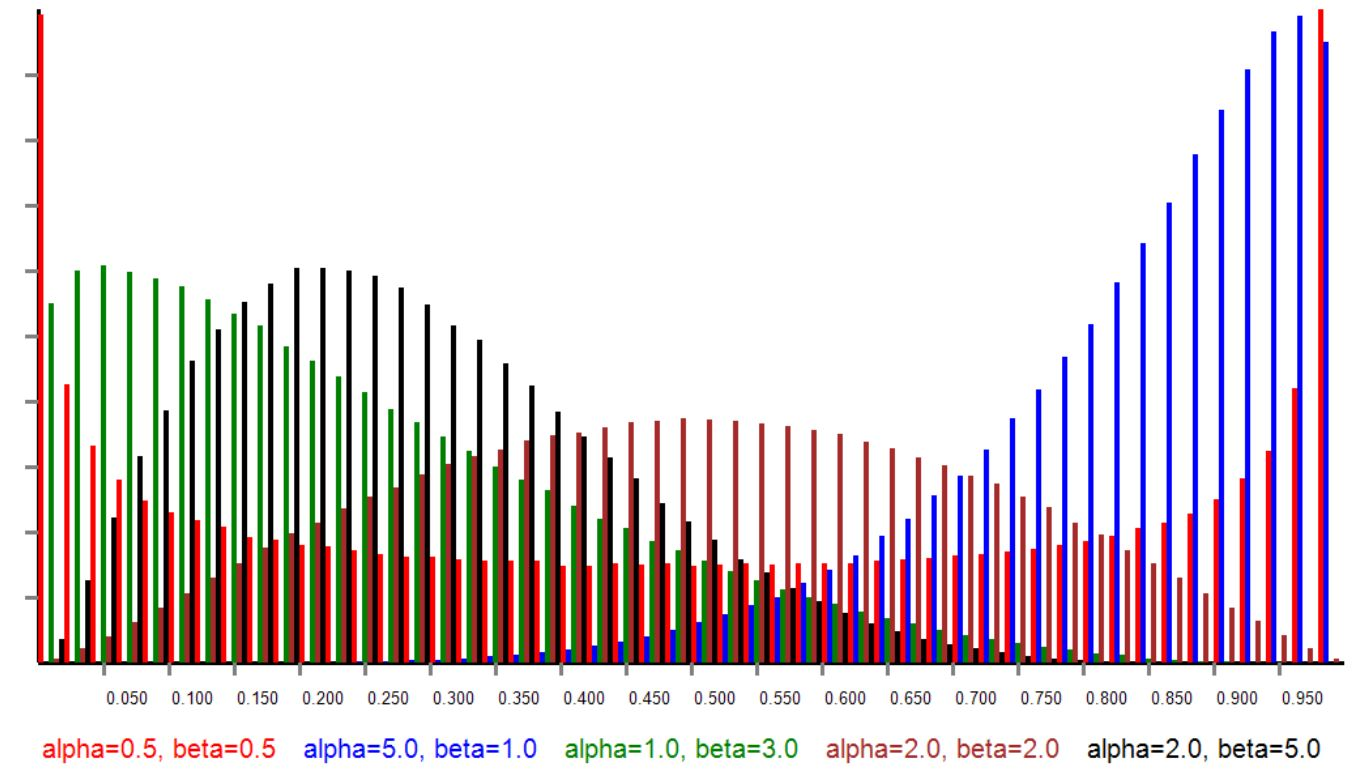
\includegraphics[width = 0.9\textwidth]{BetaDistributionSample}
\caption{从Beta分布中进行采样}
\end{figure}

\section{Dirichlet-Multinomial共轭}
给定数据集$C={c_1,c_2,...,c_n}$,$K$个不同类型出现的次数向量$\vec{N}=(n_1,n_2,...,n_K)$,以及每个类型出现概率的向量$\vec{\pi}=(\pi_0, \pi_1,...,\pi_K)$,其多项式分布的条件概率为:
\begin{displaymath}
p(C|\vec{\pi}) =p(\vec{N}|\vec{\pi})= \prod_{k=1}^{K}\pi_k^{n_k}
\end{displaymath}
参数为$\vec{A} = (a_1,a_2...a_K)$的Dirichlet分布的定义如下:
\begin{displaymath}
\begin{split}
Dir(\vec{\pi}|\vec{A})=\frac{\Gamma{(\sum_{k=1}^{K}{a_k}})}{\prod_{k=1}^{K}{\Gamma{(a_k)}}}\prod_{k=1}^{K}{\pi_{k}^{a_k-1}}
\end{split}
\end{displaymath}
当Dirichlet分布作为多项式分布的先验分布式时,其后验分布为:
\begin{displaymath}
\begin{split}
p(C|\vec{A},\vec{N})
&= \frac{p(\vec{N}|\vec{\pi}) p(\vec{\pi}|\vec{A})}{\int_{\vec{\pi}} p(\vec{M}|\vec{\pi}) p(\vec{\pi}|\vec{A})  \mathrm{d} \vec{\pi}}\\
&= \frac{
\frac{\Gamma{(\sum_{k=1}^{K}{a_k}})}{\prod_{k=1}^{K}{\Gamma{(a_k)}}}\prod_{k=1}^{K}{\pi_{k}^{a_k-1}} \prod_{k=1}^{K}\pi_k^{n_k} 
}{ \int_{\vec{\pi}}
\frac{\Gamma{(\sum_{k=1}^{K}{a_k}})}{\prod_{k=1}^{K}{\Gamma{(a_k)}}}\prod_{k=1}^{K}{\pi_{k}^{a_k-1}} \prod_{k=1}^{K}\pi_k^{n_k}   \mathrm{d} \vec{\pi}
}\\
&= \frac{
\prod_{k=1}^{K}{\pi_{k}^{a_k+n_k-1}}
}{ \int_{\vec{\pi}}
\prod_{k=1}^{K}{\pi_{k}^{a_k+n_k-1}}   \mathrm{d} \vec{\pi}
}
= \frac{
\prod_{k=1}^{K}{\pi_{k}^{a_k+n_k-1}}
}{ 
\frac{\prod_{k=1}^{K} \Gamma(a_k+n_k)}{\Gamma(\sum_{k=1}^K(a_k+n_k))}
}\\
&= \frac{\Gamma{(\sum_{k=1}^{K}{(a_k+n_k)}})}{\prod_{k=1}^{K}{\Gamma{(a_k+n_k)}}}\prod_{k=1}^{K}{\pi_{k}^{a_k+n_k-1}}\\
&= Dir(\vec{\pi}|\vec{A}+\vec{N})\\
\end{split}
\end{displaymath}
即:给定一个Dirichlet分布的先验和一个多项式分布的条件概率,可以得到一
个Dirichlet分布的一个后验。

\begin{displaymath}
\begin{split}
&\int_{\vec{\pi}} \frac{\Gamma{(\sum_{k=1}^{K}{a_k}})}{\prod_{k=1}^{K}{\Gamma{(a_k)}}}  \prod_{k=1}^{K}{\pi_{k}^{a_k-1}}   \mathrm{d} \vec{\pi} =1 \\
\to & \frac{\Gamma{(\sum_{k=1}^{K}{a_k}})}{\prod_{k=1}^{K}{\Gamma{(a_k)}}} \int_{\vec{\pi}}  \prod_{k=1}^{K}{\pi_{k}^{a_k-1}}   \mathrm{d} \vec{\pi} =1 \\
\to &  \int_{\vec{\pi}}  \prod_{k=1}^{K}{\pi_{k}^{a_k-1}}   \mathrm{d} \vec{\pi} =  \frac{\prod_{k=1}^{K}{\Gamma{(a_k)}}}  {\Gamma{(\sum_{k=1}^{K}{a_k}})}\\
\end{split}
\end{displaymath}


\begin{figure}[htbp]
\centering
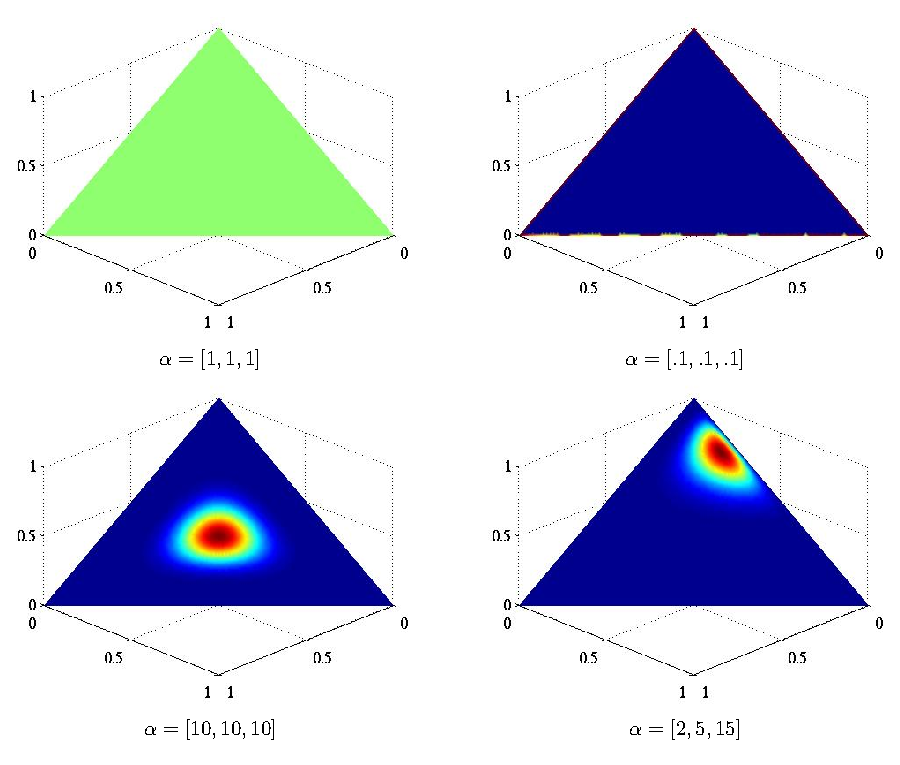
\includegraphics[width = 0.8\textwidth]{DirichletDistribution}
\caption{Dirichlet Distribution}
\end{figure}

对于一个对称的狄利克雷分布
\begin{displaymath}
\begin{split}
p(\pi_1,...,\pi_k|a)&=Dir(a/k, ... ,a/k) = \frac{\Gamma{(a)}}{{\Gamma{(a/k)}}^k} \prod_{j=1}^{k}{\pi_{j}^{a/k-1}}\\
p(C|a) &= \frac{\Gamma{a}}{\Gamma(a/k)^k} \int \prod_{j=1}^{k} \pi_j^{n_j+a/k-1} \mathrm{d} \pi_j\\
&= \frac{\Gamma{(a)}}{\Gamma(a/k)^k} \frac{\prod_{j=1}^{k}{\Gamma{(a/k +n_j)}}}  {\Gamma{(a + n)}}\\
&= \frac{\Gamma{(a)}}{\Gamma(a+n)} \prod_{j=1}^{k} \frac{\Gamma{(a/k +n_j)}} {\Gamma{(a/k)}}\\
\end{split}
\end{displaymath}

则:
\begin{displaymath}
\begin{split}
p(c_i=j|\mathbf{c}_{-i},a) &= \frac{p(\mathbf{c}|a)}{p(\mathbf{c}_{-i}|a)}\\
&= \frac{ \frac{\Gamma{(a)}}{\Gamma(a+n)} \prod_{j=1}^{k} \frac{\Gamma{(a/k +n_j)}} {\Gamma{(a/k)}}
}{\frac{\Gamma{(a)}}{\Gamma(a+n-1)}  \frac{\Gamma{(a/k +n_{j, -i})}} {\Gamma{(a/k)}} \prod_{j' \neq j} \frac{\Gamma{(a/k +n_{j'})}} {\Gamma{(a/k)}}
}\\
&= \frac{\Gamma{(n+a-1)}}{\Gamma(a+n)} \frac{\frac{\Gamma{(a/k +n_{j})}} {\Gamma{(a/k)}}}{\frac{\Gamma{(a/k +n_{j, -i})}} {\Gamma{(a/k)}}}\\
&= \frac{\Gamma{(n+a-1)}}{\Gamma(a+n)} \frac{\Gamma{(a/k +n_{j})}} {\Gamma{(a/k +n_{j, -i})}} \\
&= \frac{\Gamma{(n+a-1)}}{\Gamma(a+n)} \frac{\Gamma{(a/k +n_{j, -i} +1)}} {\Gamma{(a/k +n_{j, -i})}} \\
&= \frac{n_{j, -i} + a/k}{n+a-1}\\
\end{split}
\end{displaymath}


\subsection{Sample from Dirichlet Distribution}

如何从参数为$\vec{A} = (a_1,a_2...a_K)$的Dirichlet分布$Dir(\vec{\pi}|\vec{A})$中采样一个$\vec{\pi}$呢?

\textbf{Polya's Urn}
 
我们首先介绍一种简单的方法,即Polya's Urn。
如图所示,我们首先在一个桶中放入$K$种颜色的球各$\vec{A} = (a_1,a_2...a_K)$个,然后我们随机的从桶中拿一个球,并额外拿一个同样颜色的球,一并放回桶中,我们一直重复这个过程,可以证明,当这个操作趋向于无穷次时,桶里的球的分布将逼近一个从狄利克雷分布上的一个采样。

\begin{figure}[htbp]
\centering
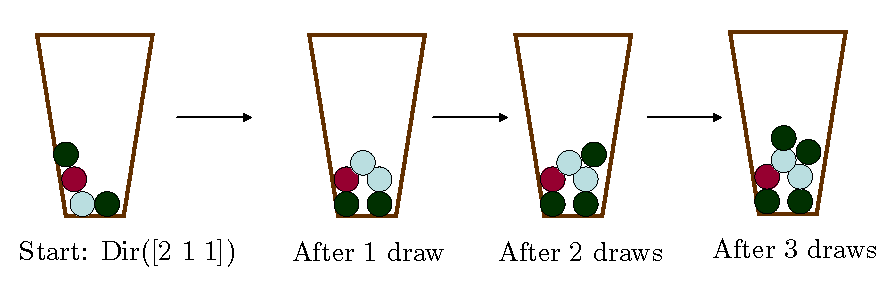
\includegraphics[width = 0.8\textwidth]{Urn-Drawing}
\end{figure}

\textbf{Stick-Breaking}

我们先来说$K=3$的情况,即 $\vec{A} = (a_1,a_2,a_3)$。我们首先从Beta分布$Beta(a_1, a_2+a_3)$中采样一个值$u_1$,并进一步的从Beta分布$Beta(a_2,a_3)$中采样一个值$u_2$,那么$(u_1, (1-u_1)u_2, 1-u_1-(1-u_1)u_2)$便是狄利克雷分布$Dir(\vec{\pi}|(a_1,a_2,a_3))$的一个采样。

\begin{figure}[htbp]
\centering
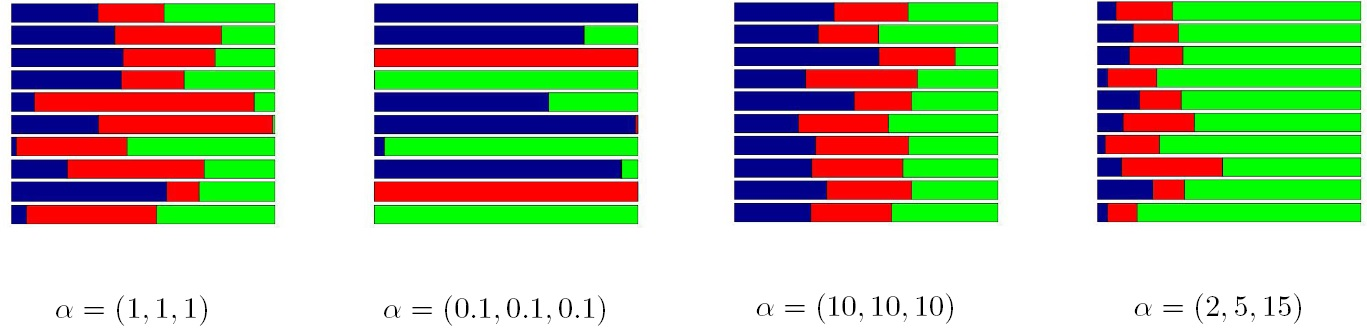
\includegraphics[width = 1.0\textwidth]{StickBreaking}
\end{figure}

当$K>3$时,我们首先从Beta分布$Beta(a_1, \sum_{2}^{k}a_k)$中采样一个值$u_1$,则剩余的棍的长度为$1-u_1$。对于$1<j<k$,如果长度$u_1,u_2,...,u_{j-1}$已经产生,则剩余棍的长度为:$\prod_{i=1}^{j-1}(1-u_i)$,我们从Beta分布$Beta(a_j, \sum_{i=j+1}^{k}a_i)$中采样一个$u_j$,并令$q_j=u_j\prod_{i=1}^{j-1}(1-u_i)$,则剩余的长度为$\prod_{i=1}^{j-1}(1-u_i) - u_j\prod_{i=1}^{j-1}(1-u_i) = \prod_{i=1}^{j}(1-u_i)$。令剩余长度为$q_k$,则$(q_1. q_2,...,q_k)$是狄利克雷分布$Dir(\vec{\pi}|(a_1,a_2,...,a_k))$的一个采样。

\begin{figure}[htbp]
\centering
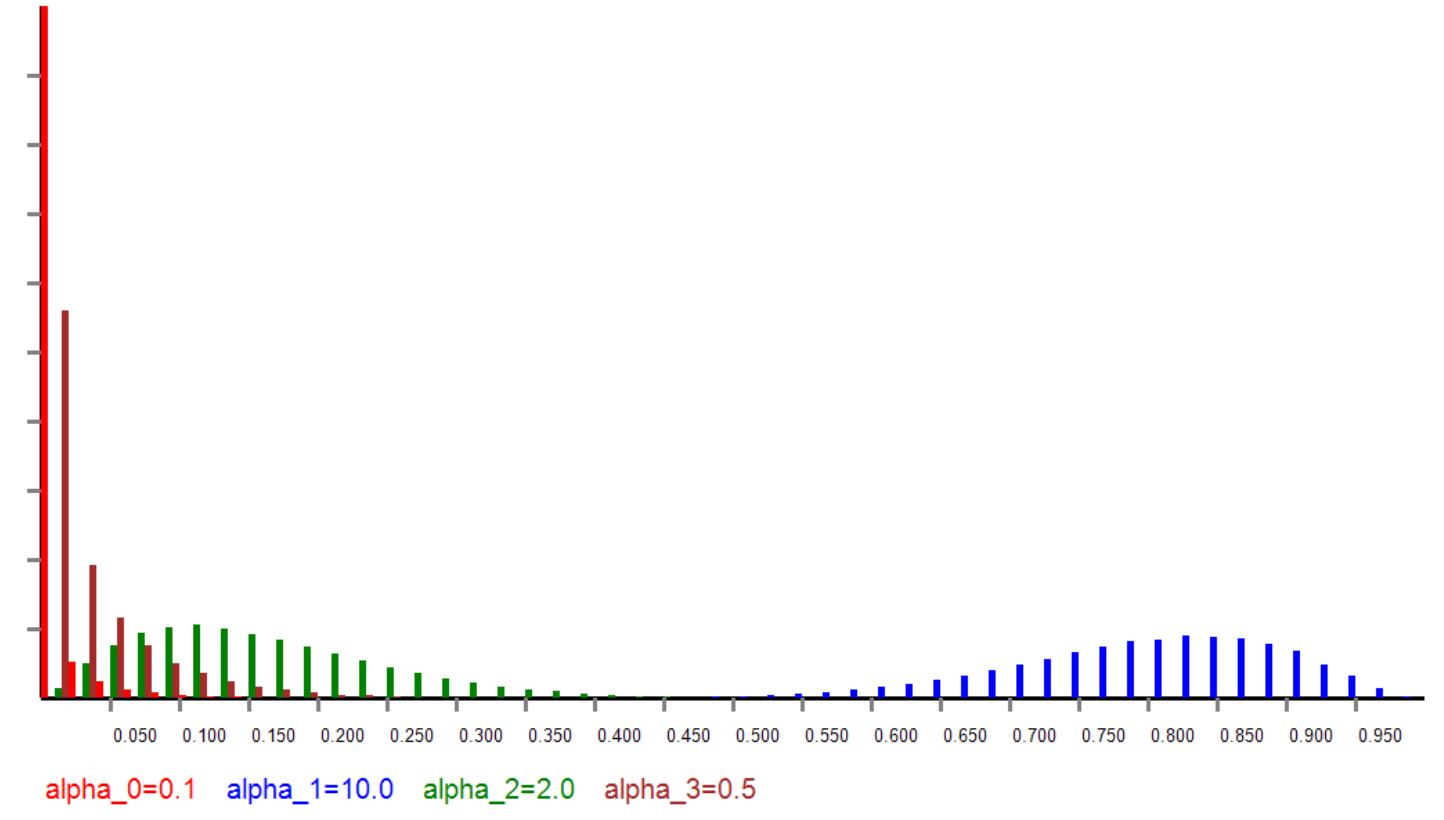
\includegraphics[width = 0.9\textwidth]{DirichletDistributionSample}
\caption{从Dirichlet分布中进行采样}
\end{figure}
% !Mode:: "TeX:UTF-8"

\chapter{SVM}

\section{不带松弛因子的SVM}
样本点$x_i$到直线$y=wx+b$的距离为:
\begin{displaymath}
\frac{wx_i+b}{\| w \|}
\end{displaymath}  
 
样本点$x_i$到直线$y=wx+b$的几何距离为:
\begin{displaymath}
\frac{y_i*(wx_i+b)}{\| w \|}
\end{displaymath} 

不失一般性的假设样本集合中距离分类面$y=wx+b$的距离最小的样本为
$(x_i,y_i)$,则假设其算术距离为1,即:
\begin{displaymath}
y_i*(wx_i+b)=1
\end{displaymath} 

那么,SVM的优化目标变为:$argmax{\frac{1}{\|w\|}}$
给定: $min_i(y_i*(wx_i+b)) = 1$
即: $y_i*(wx_i+b) \geq 1$

又:$argmax{\frac{1}{\|w\|}} = argmin(\frac{1}{2}\|w\|) =
argmin(\frac{1}{2}w^2)$

有带约束问题的极值:
\begin{equation}
argmin(\frac{1}{2}w^2 - \sum_i{\lambda_i(y_i*(wx_i+b)-1)})
\end{equation} 

其为凸函数,对$w$求导为0得:
\begin{equation}
w = \sum_i{\lambda_i(y_i*x_i)}
\end{equation} 

对$b$求导为0得:
\begin{equation}
 \sum_i{\lambda_i*y_i}=0
\end{equation}

将求得的$w$代入原公式的:
\begin{equation}
\begin{split}
&\frac{1}{2}w^2 - \sum_i{\lambda_i(y_i*(wx_i+b)-1)}\\
&=\frac{1}{2}(\sum_i{\lambda_i(y_i*x_i)})(\sum_j{\lambda_j(y_j*x_j)}) -
\sum_i{\lambda_i(y_i*((\sum_i{\lambda_j(y_j*x_j)})x_i+b)-1)}\\
&=-\frac{1}{2}\sum_i\sum_j{\lambda_i\lambda_jy_iy_jx_ix_j}
-\sum_i{\lambda_i(y_ib)}+\sum_i{\lambda_i}\\
&\sum_i{\lambda_i*y_i}=0\\
&=\sum_i{\lambda_i}-\frac{1}{2}\sum_i\sum_j{\lambda_i\lambda_jy_iy_jx_ix_j}
\end{split}
\end{equation}

故原始最优化问题转换为:
\begin{equation}
argmin_\lambda{\sum_i{\lambda_i}-\frac{1}{2}\sum_i\sum_j{\lambda_i\lambda_jy_iy_jx_ix_j}}
\end{equation}
subject to: $ \sum_i{\lambda_i*y_i}=0$ and $\lambda_i \geq 0$。称为原
始问题的对偶形式。

该受限极值问题为二次规划问题,可以用 Sequential Minimal Optimization
(SMO)方法求解。

\section{带松弛因子的SVM}
为了处理线性不可分的情况,引入松弛变量$\xi \geq 0$,从而允许某些样本点到分类面的函数距离少于1,即
\begin{equation}
 y_i*(wx_i+b) \geq 1-\xi_i
\end{equation}
注意,每个样本点可选择不同的$\xi$,该参数会被模型优化。

为了使得松弛变量$\xi_i$越小越好,将优化目标变为:
\begin{displaymath}
argmin_w{\frac{1}{2}*w^2} + C\sum_i{\xi_i}
\end{displaymath} 

引入拉格朗日算子,将受限极值转换为非受限极值:
\begin{equation}
argmin{\frac{1}{2}w^2  + C\sum_i{\xi_i} -
\sum_i{\lambda_i(y_i*(wx_i+b)-1+\xi_i)} - \sum_i{\beta_i\xi_i}}
\end{equation} 

函数为凸,对$w$,$b$,$\xi$求导为0得:
\begin{equation}
w = \sum_i{\lambda_i(y_i*x_i)}
\end{equation} 
\begin{equation}
 \sum_i{\lambda_i*y_i}=0
\end{equation}

\begin{equation}
C-\lambda_i-\beta_i=0 \Longrightarrow
C-\lambda_i = \beta_i
\end{equation}

将求导所得代入原始公式得原始问题的对偶形式:
\begin{equation}
argmin_\lambda{\sum_i{\lambda_i}-\frac{1}{2}\sum_i\sum_j{\lambda_i\lambda_jy_iy_jx_ix_j}}
\end{equation}
subject to:
\begin{equation}
\begin{split} 
\sum_i{\lambda_i*y_i} &=0\\
\lambda_i &\geq 0 \\
\left\{
\begin{aligned}
 C-\lambda_i &=& \beta_i\\
\beta_i &\geq& 0
\end{aligned}
\right\}
\Longrightarrow
C-\lambda_i \geq 0 \Longrightarrow \lambda_i \leq C
\end{split}
\end{equation}

比较引入松弛变量$\xi_i$的最后结果同引入前的相比,差别仅仅在于对
$\lambda_i$的约束上,最后的模型并没有保留任何松弛变量。

% !Mode:: "TeX:UTF-8"

\chapter{熵(Entropy)}

\section{什么是熵}

\section{相对熵}

\section{最大熵}


% !Mode:: "TeX:UTF-8"
\chapter{EM 和 GMM}

% !Mode:: "TeX:UTF-8"

\section{EM}


参数为$\theta$,样本$x_i$的概率为$p(x_i;\theta)$,隐变量为$z$,则最大似
然为:
\begin{displaymath}
\begin{split}
\ell(\theta) &= \sum_{i=1}^{n}{log(p(x_i;\theta))}\\
&= \sum_{i=1}^{n}{log(\sum_{z}{p(x_i,z;\theta)})}
\end{split}
\end{displaymath} 

令$\Theta(z)$为隐变量$z$的分布,则:
\begin{displaymath}
\begin{split}
\ell(\theta) &= \sum_{i=1}^{n}{log(\sum_{z}{p(x_i,z;\theta)})}\\
&=
\sum_{i=1}^{n}{log(\sum_{z}{(\Theta(z)*\frac{p(x_i,z;\theta)}{\Theta(z)}}))}\\
&\geq \sum_{i=1}^{n}{\sum_{z}{\Theta(z)*log(\frac{p(x_i,z;\theta)}{\Theta(z)}})}
\end{split}
\end{displaymath} 
最后一步为Jesen不等式。有公式可以看到,最大似然$\ell(\theta)$的下界为
$\frac{p(x_i,z;\theta)}{\Theta(z)}$的期望。

我们可以选择一个合适的隐状态的分布$\Theta(z)$使得不等式的等号成立,根
据Jesen不等式成立的条件,对每个不同的$i$,$log$内部的$\frac{p(x_i,z;\theta)}{\Theta(z)}$为常数
$C_i$,即$\frac{p(x_i,z;\theta)}{\Theta(z)}$不随$z$的变化而变化,得:
$\frac{p(x_i,z;\theta)}{\Theta(z)} = C_i$
而又有 $\sum_{z}{\Theta(z)}=1$,从而:
\begin{displaymath}
\sum_{z}{p(x_i,z;\theta)} = \sum_{z}{\Theta(z)*C_i}
=C_i
=p(x_i;\theta)
\end{displaymath} 
故而:
\begin{displaymath}
\begin{split}
\Theta(z) &= \frac{p(x_i,z;\theta)}{p(x_i;\theta)}\\
&=p(z|x_i;\theta)
\end{split}
\end{displaymath} 
即,当隐状态$z$的分布$\Theta(z)$取最大似然估计的结果$p(z|x_i;\theta)$时,
不等式的等号成立:样本$x$的最大似然概率等于
$\frac{p(x_i,z;\theta)}{\Theta(z)}$的期望。

目前为止,给定了样本$x$和参数$\theta$,我们可以用最大似然来获得隐状态
分布$\Theta(z)$,而给定了样本$x$和隐状态的分布$\Theta(z)$,我们又可以
通过最大化样本的似然概率来获得参数$\theta$。故而,EM训练的过程为:

E步:选择一个合适的隐状态的分布$\Theta(z)$,使得样本$x$的最大似然概率
等于Jesen不等式得到的下界,即$\frac{p(x_i,z;\theta)}{\Theta(z)}$的期望。根据Jesen不等式成立的
条件,给定样本$x$和参数$\theta$的情况下,隐状态的分布为:
\begin{displaymath}
\Theta(z)=p(z|x_i;\theta)
\end{displaymath} 

M步:最大化Jesen不等式得到的下界,来求得参数$\theta$,即:
\begin{displaymath}
\begin{split}
\theta &= argmax{\sum_{i=1}^{n}{\sum_{z}{\Theta(z)*log(\frac{p(x_i,z;\theta)}{\Theta(z)}})}}
\end{split}
\end{displaymath} 

Jessen不等式理解:令$\frac{p(x_i,z;\theta)}{\Theta(z)} = x_z$,则有:
\begin{displaymath}
\begin{split}
log(\sum_{z}{(\Theta(z)*\frac{p(x_i,z;\theta)}{\Theta(z)}})) &=log(\sum_{z}{(\Theta(z)*x_z}))\\
&=log(\Theta_{0}x_0 + \Theta_{1}x_1 +\Theta_{2}x_2+...+\Theta_{n}x_n)\\
&\geq \Theta_0log(x_0) + \Theta_1log(x_1) +\Theta_2log(x_2)+...+\Theta_nlog(x_n)\\
&=\sum_{z}{\Theta(z)*log(x_z)}\\
&=\sum_{z}{(\Theta(z)*log(\frac{p(x_i,z;\theta)}{\Theta(z)})})\\
\end{split}
\end{displaymath} 

当$x_z=C$,且$sum_{z}{\Theta(z)} = 1$(概率分布的性质)时,
\begin{displaymath}
\begin{split}
log(\sum_{z}{(\Theta(z)*x_z})) = log(1*C) &=log(C)\\
\sum_{z}{\Theta(z)*log(x_z)} = 1*log(C)&=log(C)
\end{split}
\end{displaymath} 

% !Mode:: "TeX:UTF-8"

\section{GMM}

高斯混合模型的定义为若干高斯模型的线性加权,如下:
\begin{displaymath}
\begin{split}
&p(z_k)=\pi_k\\
&p(x_{i}|z_k)=\mathcal{N}(x_{i}|\mathbf{\mu}_k,\mathbf{\varSigma}_k) = 
\frac{exp\Big{\{}
-\frac{1}{2}(x_i-\mu_k)^T\varSigma_k^{-1}(x_i-\mu_k)
\Big{\}}}{(2\pi)^{\frac{D}{2}}|\varSigma_k|^{\frac{1}{2}}} 
\\
&p(x_{i})=\sum_{k}^{K}{p(z_k)}p(x_{i}|z_k)=\sum_{k=1}^{K}\pi_k\mathcal{N}(x_{i}|\mathbf{\mu}_k,\mathbf{\varSigma}_K)\\
&p(z_k|x_{i})
=\frac{p(z_k)p(x_{i}|z_k)}{\sum_{k'=1}^{K}p(z_{k'})p(x_{i}|z_{k'})} =\frac{
\pi_k\mathcal{N}(x_{i}|\mathbf{\mu}_k,\mathbf{\varSigma}_k)
}{
\sum_{k'=1}^{K}\pi_{k'}\mathcal{N}(x_{i}|\mathbf{\mu}_{k'},\mathbf{\varSigma}_{k'})
}
\end{split}
\end{displaymath}

观测样本$\mathbf{x}$的对数似然函数为:
\begin{displaymath}
\begin{split}
\log p(\mathbf{x}) &=\log \Big{\{} \prod_{i=1}^N{p(x_i)}\Big{\}}\\
&=\sum_{i=1}^{N} \log \Bigg{\{} \sum_{k=1}^{K}\{p(x_i,z_k)\}
\Bigg{\}}\\
&=\sum_{i=1}^{N} \log \Bigg{\{} \sum_{k=1}^{K}\{\mathcal{Q}(z_k)\frac{p(x_i,z_k)}{\mathcal{Q}(z_k)}\} \Bigg{\}}\\
&\geq \sum_{i=1}^{N} \sum_{k=1}^{K} \Bigg{\{}
\mathcal{Q}(z_k) \log \{ \frac{p(x_i,z_k)} {\mathcal{Q}(z_k)}  \}
\Bigg{\}}\\
\end{split}
\end{displaymath}

Jessen不等式成立的条件是对每个不同的$i$,$\frac{p(x_i,z_k)} {\mathcal{Q}(z_k)} $为常数
$C_i$,故$p(x_i,z_k) =C_i \times \mathcal{Q}(z_k)$:

\begin{displaymath}
\begin{split}
\sum_{k=1}^{K}p(x_i,z_k) =C_i \times \sum_{k=1}^{K}\mathcal{Q}(z_k)
&\Longrightarrow C_i = \sum_{k=1}^{K}p(x_i,z_k) = p(x_i) \\
\mathcal{Q}(z_k) = \frac{p(x_i,z_k)}{p(x_i)} &= p(z_k|x_i) = w_{k,i}
\end{split}
\end{displaymath}
故而得到E步的更新公式为:
\begin{displaymath}
\begin{split}
\mathcal{Q}(z_k) &= w_{k,i} = p(z_k|x_i)\\
&= \frac{
\pi_k\mathcal{N}(x_{i}|\mathbf{\mu}_k,\mathbf{\varSigma}_k)
}{
\sum_{k'=1}^{K}\pi_{k'}\mathcal{N}(x_{i}|\mathbf{\mu}_{k'},\mathbf{\varSigma}_{k'})
}
\end{split}
\end{displaymath}

我们现在最大化由Jessen不等式得到的下界:
\begin{displaymath}
\begin{split}
max \Bigg{\{} 
\sum_{i=1}^{N} \sum_{k=1}^{K} \Bigg{\{}
w_{k,i} \log \{ \frac{p(x_i,z_k)} {w_{k,i}}  \}
\Bigg{\}}
\end{split}
\end{displaymath}
subject to:
\begin{displaymath}
\sum_{k=1}^{K}{\pi_k} = 1
\end{displaymath}

引入拉格朗日算子得:
\begin{displaymath}
\begin{split}
&\mathop{\arg\max}_{\pi,\mu, \varSigma} \Bigg{\{} 
\sum_{i=1}^{N} \sum_{k=1}^{K} \Bigg{\{}
w_{k,i} \log \{ \frac{p(x_i,z_k)} {w_{k,i}}  \}
-\lambda \Big{\{} \sum_{k=1}^{K}{\pi_k}-1 \Big{\}}
\Bigg{\}}\\
&=\mathop{\arg\max}_{\pi,\mu, \varSigma} \Bigg{\{} 
\sum_{i=1}^{N} \sum_{k=1}^{K} \Bigg{\{}
w_{k,i} \log \{ \frac{p(x_i|z_k)p(z_k)} {w_{k,i}}  \}
-\lambda \Big{\{} \sum_{k=1}^{K}{\pi_k}-1 \Big{\}}
\Bigg{\}}\\
&=\mathop{\arg\max}_{\pi,\mu, \varSigma} \Bigg{\{} 
\sum_{i=1}^{N} \sum_{k=1}^{K} 
\Bigg{\{}
w_{k,i} \log \{ \frac{\pi_k \mathcal{N}(x_{i}|\mu_k,\varSigma_k)} {w_{k,i}}  \}
-\lambda \Big{\{} \sum_{k=1}^{K}{\pi_k}-1 \Big{\}}
\Bigg{\}}\\
&=\mathop{\arg\max}_{\pi,\mu, \varSigma} \Bigg{\{} 
\sum_{i=1}^{N} \sum_{k=1}^{K} 
\Bigg{\{}
w_{k,i} \{ 
\log{\pi_k} + \log{\mathcal{N}(x_{i}|\mu_k,\varSigma_k)}-\log{w_{k,i}}  
\}
-\lambda \Big{\{} \sum_{k=1}^{K}{\pi_k}-1 
\Big{\}}
\Bigg{\}}\\
&=\mathop{\arg\max}_{\pi,\mu, \varSigma} \Bigg{\{} 
\sum_{i=1}^{N} \sum_{k=1}^{K} 
\Bigg{\{}
w_{k,i} \{ 
\log{\pi_k} + \log{\mathcal{N}(x_{i}|\mu_k,\varSigma_k)} 
\}
-\lambda \sum_{k=1}^{K}{\pi_k} 
\Bigg{\}}\\
\end{split}
\end{displaymath}

对$\pi_k$求导为0得:
\begin{displaymath}
\begin{split}
&\frac{\sum_{i=1}^{N}{w_{k,i}}}{\pi_k}-\lambda = 0\\
\Longrightarrow & \sum_{k=1}^{K} \sum_{i=1}^{N} {w_{k,i}} =
\sum_{k=1}^{K}{\lambda \pi_k}\\
\Longrightarrow & \lambda = \sum_{k=1}^{K} \sum_{i=1}^{N} {w_{k,i}} =
N\\
\Longrightarrow & \pi_k = \frac{1}{N}\sum_{i=1}^{N}{w_{k,i}}
\end{split}
\end{displaymath}


令 $C=exp\{-\frac{1}{2}(x_i-\mu_k)\varSigma_k^{-1}(x_i-\mu_k)^T\}$,则:
\begin{displaymath}
\begin{split}
&\frac{dC}{d\mu_k} = C \varSigma_k^{-1}(x_i-\mu_k)^T\\
&\frac{d \mathcal{N}(x_{i}|\mathbf{\mu}_k,\mathbf{\varSigma}_k)}{d\mu_k} = \mathcal{N}(x_{i}|\mathbf{\mu}_k,\mathbf{\varSigma}_k) \varSigma_k^{-1}(x_i-\mu_k)^T\\
\end{split}
\end{displaymath}



对$\mu_k$求导为0得:
\begin{displaymath}
\begin{split}
&\frac{
\delta{ \Bigg{(}
\sum_{i=1}^{N} \sum_{k=1}^{K} 
\Bigg{\{}
w_{k,i} \{ 
\log{\pi_k} + \log{\mathcal{N}(x_{i}|\mu_k,\varSigma_k)} 
\}
-\lambda \sum_{k=1}^{K}{\pi_k} \Bigg{\}} \Bigg{)}
}}{\delta{\mu_k}} = 0\\
\Longrightarrow& \frac{
\delta{ \Bigg{(}
\sum_{i=1}^{N} \sum_{k=1}^{K} 
\Bigg{\{}
w_{k,i} \log{\mathcal{N}(x_{i}|\mu_k,\varSigma_k)} 
\Bigg{\}} \Bigg{)}
}}{\delta{\mu_k}} = 0\\
\Longrightarrow& \frac{
\delta{ \Bigg{(}
\sum_{i=1}^{N}
\Bigg{\{}
w_{k,i} \log{\mathcal{N}(x_{i}|\mu_k,\varSigma_k)} 
\Bigg{\}} \Bigg{)}
}}{\delta{\mu_k}} = 0\\
\Longrightarrow& 
\sum_{i=1}^{N}
\Bigg{\{}
w_{k,i} 
\frac{
      \frac{
           \delta(  \mathcal{N}(x_{i}|\mu_k,\varSigma_k)  )
           }{\delta{\mu_k}}
}
{\mathcal{N}(x_{i}|\mu_k,\varSigma_k)} 
\Bigg{\}}
 = 0\\
\end{split}
\end{displaymath}

由于 $b\frac{d
  \mathcal{N}(x_{i}|\mathbf{\mu}_k,\mathbf{\varSigma}_k)}{d\mu_k} =
\mathcal{N}(x_{i}|\mathbf{\mu}_k,\mathbf{\varSigma}_k)
\varSigma_k^{-1}(x_i-\mu_k)^T$:
\begin{displaymath}
\begin{split}
\Longrightarrow& 
\sum_{i=1}^{N}
\Bigg{\{}
w_{k,i} 
\frac{
 \mathcal{N}(x_{i}|\mathbf{\mu}_k,\mathbf{\varSigma}_k) \varSigma_k^{-1}(x_i-\mu_k)^T
}
{\mathcal{N}(x_{i}|\mu_k,\varSigma_k)} 
\Bigg{\}}
 = 0\\
\Longrightarrow& 
\sum_{i=1}^{N}
\Bigg{\{}
w_{k,i}  \varSigma_k^{-1}(x_i-\mu_k)^T
\Bigg{\}}
 = 0\\
\Longrightarrow& 
\sum_{i=1}^{N}
\Bigg{\{}
w_{k,i}(x_i-\mu_k)
\Bigg{\}}
 = 0\\
\Longrightarrow& 
\sum_{i=1}^{N}
\Bigg{\{}
w_{k,i}x_i
\Bigg{\}}
 = \sum_{i=1}^{N}
\Bigg{\{}
w_{k,i}\mu_k
\Bigg{\}}\\
\Longrightarrow& 
\mu_k = \frac{
\sum_{i=1}^{N}  w_{k,i}x_i 
}{ 
\sum_{i=1}^{N} w_{k,i}
}\\
\end{split}
\end{displaymath}


先列几个下边会用到的求导公式:
\begin{displaymath}
\begin{split}
&\frac{d|M|}{dM} = |M|(M^{-1})^T\\
&\frac{\delta(a^TMb)}{dM} = ab^T\\
\end{split}
\end{displaymath}

令 $C=exp\{-\frac{1}{2}(x_i-\mu_k)\varSigma_k^{-1}(x_i-\mu_k)^T\}$,则:
\begin{displaymath}
\begin{split}
\frac{dC}{d\varSigma_k^{-1}} &= C (-\frac{1}{2})(x_i-\mu_k)(x_i-\mu_k)^T\\
\frac{d
  \mathcal{N}(x_{i}|\mathbf{\mu}_k,\mathbf{\varSigma}_k)}{d\varSigma_k^{-1}}
&= \frac{C}{(2\pi)^{\frac{D}{2}}}
\frac{\delta{(|\varSigma_k^{-1}|^{\frac{1}{2}})}}{\delta{\varSigma_k^{-1}}}
+ \frac{|\varSigma_k^{-1}|^{\frac{1}{2}}}{(2\pi)^{\frac{D}{2}}}
\frac{\delta{C}}{\delta{\varSigma_k^{-1}}}
\\
&= \frac{C}{(2\pi)^{\frac{D}{2}}}
\frac{|\varSigma_k^{-1}|^{-\frac{1}{2}}|\varSigma_k^{-1}|\varSigma_k}{2}
+ \frac{|\varSigma_k^{-1}|^{\frac{1}{2}}}{(2\pi)^{\frac{D}{2}}}
 C (-\frac{1}{2})(x_i-\mu_k)(x_i-\mu_k)^T
\\
&= \frac{C|\varSigma_k^{-1}|^{\frac{1}{2}}\varSigma_k}{2(2\pi)^{\frac{D}{2}}}
- \frac{C|\varSigma_k^{-1}|^{\frac{1}{2}}(x_i-\mu_k)(x_i-\mu_k)^T}
{2(2\pi)^{\frac{D}{2}}}
\\
&= \frac{C|\varSigma_k^{-1}|^{\frac{1}{2}} 
(\varSigma_k - (x_i-\mu_k)(x_i-\mu_k)^T)
}{2(2\pi)^{\frac{D}{2}}}
\\
&=  \frac{1}{2}\mathcal{N}(x_{i}|\mu_k,\varSigma_k)
(\varSigma_k - (x_i-\mu_k)(x_i-\mu_k)^T)
\\
\end{split}
\end{displaymath}

对$\varSigma_k$求导为0得:
\begin{displaymath}
\begin{split}
&\frac{
\delta{ \Bigg{(}
\sum_{i=1}^{N} \sum_{k=1}^{K} 
\Bigg{\{}
w_{k,i} \{ 
\log{\pi_k} + \log{\mathcal{N}(x_{i}|\mu_k,\varSigma_k)} 
\}
-\lambda \sum_{k=1}^{K}{\pi_k} \Bigg{\}} \Bigg{)}
}}{\delta{\varSigma_k}} = 0\\
\Longrightarrow& \frac{
\delta{ \Bigg{(}
\sum_{i=1}^{N} \sum_{k=1}^{K} 
\Bigg{\{}
w_{k,i} \log{\mathcal{N}(x_{i}|\mu_k,\varSigma_k)} 
\Bigg{\}} \Bigg{)}
}}{\delta{\varSigma_k}} = 0
\end{split}
\end{displaymath}

\begin{displaymath}
\begin{split}
\Longrightarrow& \frac{
\delta{ \Bigg{(}
\sum_{i=1}^{N}
\Bigg{\{}
w_{k,i} \log{\mathcal{N}(x_{i}|\mu_k,\varSigma_k)} 
\Bigg{\}} \Bigg{)}
}}{\delta{\varSigma_k}} = 0 \\
\Longrightarrow &
\sum_{i=1}^{N}
\Bigg{\{}
w_{k,i} 
\frac{
      \frac{
           \delta(  \mathcal{N}(x_{i}|\mu_k,\varSigma_k)  )
           }{\delta{\varSigma_k}}
}
{\mathcal{N}(x_{i}|\mu_k,\varSigma_k)} 
\Bigg{\}}
 = 0\\
\end{split}
\end{displaymath}

由于 $b\frac{d
  \mathcal{N}(x_{i}|\mathbf{\mu}_k,\mathbf{\varSigma}_k)}{d\varSigma_k} =
 \frac{1}{2}\mathcal{N}(x_{i}|\mu_k,\varSigma_k)
(\varSigma_k - (x_i-\mu_k)(x_i-\mu_k)^T)$:
\begin{displaymath}
\begin{split}
\Longrightarrow& 
\sum_{i=1}^{N}
\Bigg{\{}
w_{k,i} 
\frac{
\frac{1}{2}\mathcal{N}(x_{i}|\mu_k,\varSigma_k)
(\varSigma_k - (x_i-\mu_k)(x_i-\mu_k)^T)
}
{\mathcal{N}(x_{i}|\mu_k,\varSigma_k)} 
\Bigg{\}}
 = 0\\
\Longrightarrow& 
\sum_{i=1}^{N}
\Bigg{\{}
w_{k,i}\varSigma_k
\Bigg{\}}
 = \sum_{i=1}^{N}
\Bigg{\{}
w_{k,i}(x_i-\mu_k)(x_i-\mu_k)^T
\Bigg{\}}
\\
\Longrightarrow& 
\varSigma_k = \frac{
\sum_{i=1}^{N}  w_{k,i} (x_i-\mu_k)(x_i-\mu_k)^T
}{ 
\sum_{i=1}^{N} w_{k,i}
}\\
\end{split}
\end{displaymath}

综上,GMM模型使用EM进行训练时的步骤为:

E步:选择一个合适的隐状态的分布$\Theta(z_k)$,使得样本$x$的最大似然概率
等于Jesen不等式得到的下界,即$\frac{p(x_i,z_k)} {\mathcal{Q}(z_k)}$的期望。根据Jesen不等式成立的
条件,给定样本$\mathbf{x}$和参数$\pi_k, \mu_k, \varSigma_k$的情况下,隐状态的分布为:
\begin{displaymath}
w_{k,i} = \frac{
\pi_k\mathcal{N}(x_{i}|\mathbf{\mu}_k,\mathbf{\varSigma}_k)
}{
\sum_{k'=1}^{K}\pi_{k'}\mathcal{N}(x_{i}|\mathbf{\mu}_{k'},\mathbf{\varSigma}_{k'})
}
\end{displaymath} 

M步:最大化Jesen不等式得到的下界,来求得参数$\pi_k, \mu_k, \varSigma_k$,即:
\begin{displaymath}
\begin{split}
\pi_k &= \frac{1}{N}\sum_{i=1}^{N}{w_{k,i}}\\
\mu_k &= \frac{
\sum_{i=1}^{N}  w_{k,i}x_i 
}{ 
\sum_{i=1}^{N} w_{k,i}
}\\
\varSigma_k &= \frac{
\sum_{i=1}^{N}  w_{k,i} (x_i-\mu_k)(x_i-\mu_k)^T
}{ 
\sum_{i=1}^{N} w_{k,i}
}\\
\end{split}
\end{displaymath} 



% !Mode:: "TeX:UTF-8"
\chapter{变分推断(Variational Inference)}
机器学习中一个重要的任务是需要估计一个后验分布$p(\mathbf{Z}|\mathbf{X})$(比如在EM算的E步),其中$\mathbf{X}$为观测到的数据,$\mathbf{Z}$为隐变量。然而有的时候隐变量$\mathbf{Z}$的后验分布并不是很容易的计算得到。变分推断则是一个近似的计算后验分布的方法。变分推断的基本思路是,首先引入一个简单的容易计算的分布$q(\mathbf{Z})$,然后将原分布$p(\mathbf{X})$转换为分布$q(\mathbf{Z})$的函数,并最大化以$q(\mathbf{Z})$为参数的一个下界ELOB。

\section{对数似然和ELOB下界}

\begin{displaymath}
\begin{split}
p(\mathbf{Z} | \mathbf{X}) &= \frac{ p(\mathbf{X}, \mathbf{Z})} { p(\mathbf{X}) }\\
\ln (p(\mathbf{X})) &= \ln(p(\mathbf{X}, \mathbf{Z})) - \ln(p(\mathbf{Z}|\mathbf{X}))\\
\ln (p(\mathbf{X})) &= \left [ \ln(p(\mathbf{X}, \mathbf{Z})) -\ln(q(\mathbf{Z})) \right ] - \left [ \ln(p(\mathbf{Z}|\mathbf{X})) - \ln(q(\mathbf{Z})) \right ]\\
\ln (p(\mathbf{X})) &= \ln(\frac{ p(\mathbf{X}, \mathbf{Z})}{q(\mathbf{Z})}) - \ln( \frac{p(\mathbf{Z}|\mathbf{X})}{q(\mathbf{Z})})
\end{split}
\end{displaymath}
我们对公式两边取$q(\mathbf{Z})$的期望,得:
\begin{displaymath}
\begin{split}
\int{\ln (p(\mathbf{X})) q(\mathbf{Z})} \mathrm{d}\mathbf{Z} &= \int{ \ln(\frac{ p(\mathbf{X}, \mathbf{Z})}{q(\mathbf{Z})}) q(\mathbf{Z})} \mathrm{d}\mathbf{Z}- \int {\ln( \frac{p(\mathbf{Z}|\mathbf{X})}{q(\mathbf{Z})}) q(\mathbf{Z})} \mathrm{d}\mathbf{Z}\\
\ln(p(\mathbf{X})) &=
\begin{matrix} 
\underbrace { 
\left ( \int{ q(\mathbf{Z}) \ln( p(\mathbf{X}, \mathbf{Z}))} \mathrm{d}\mathbf{Z} -
 \int{ q(\mathbf{Z}) \ln({q(\mathbf{Z})})} \mathrm{d}\mathbf{Z} \right ) 
} \\
\mathcal{L}(q)
\end{matrix}
+
\begin{matrix}
\underbrace{
 \left ( - \int {q(\mathbf{Z}) \ln( \frac{p(\mathbf{Z}|\mathbf{X})}{q(\mathbf{Z})})} \mathrm{d}\mathbf{Z} \right )
}\\
\mathbb{KL}(q\|p)
\end{matrix}
\end{split}
\end{displaymath}
我们管$\mathcal{L}(q)$叫Evidence Lower Bound(ELOB)。由上式可以看到当$\mathbb{KL}(q\|p)$为0时,$\ln(p(\mathbf{X})) = \mathcal{L}(q) $,此时$q(\mathbf{Z}) = p(\mathbf{Z}|\mathbf{X})$。

另一种证明思路:
\begin{displaymath}
\begin{split}
\ln(p(\mathbf{X})) &= \log \int {p(\mathbf{X}, \mathbf{Z})} \mathrm{d}\mathbf{Z}\\
&= \log \int {p(\mathbf{X}, \mathbf{Z}) \frac{q(\mathbf{Z})}{q(\mathbf{Z})}} \mathrm{d}\mathbf{Z}\\
&= \log \int {p(\mathbf{X}, \mathbf{Z}) \frac{q(\mathbf{Z})}{q(\mathbf{Z})}} \mathrm{d}\mathbf{Z}\\
&\geq \int { q(\mathbf{Z}) \log{\frac{p(\mathbf{X}, \mathbf{Z})}{q(\mathbf{Z})}} } \mathrm{d}\mathbf{Z}\\
&= \int{ q(\mathbf{Z}) \ln( p(\mathbf{X}, \mathbf{Z}))} \mathrm{d}\mathbf{Z} -  \int{ q(\mathbf{Z}) \ln({q(\mathbf{Z})})} \mathrm{d}\mathbf{Z}\\
&= \mathcal{L}(q)
\end{split}
\end{displaymath}
其中我们使用了Jesen不等式,由Jesen不等式成立的条件得$\frac{p(\mathbf{X}, \mathbf{Z})}{q(\mathbf{Z})}$为常数(与$\mathbf{Z}$无关),容易证明此时$q(\mathbf{Z}) = p(\mathbf{Z}|\mathbf{X})$。

\section{变分推断(Variational Inference)}
经过上边的推导,我们发现可以通过最大化ELOB来近似最大化数据的对数似然。很多情况下由于模型太多复杂导致直接最大化ELOB比较困难,变分推断的思路是,我们可以假设一个简单的容易计算的隐变量的分布$q(\mathbf{Z})$,然后训练该简单分布的参数以最大化ELOB。我们可以假设隐变量之间是相互独立的,即$q(\mathbf{Z})=\prod_{i=1}^{M}{q_i(\mathbf{Z}_i)}$。从而ELBO转换为:
\begin{displaymath}
\begin{split}
\mathcal{L}(q) &= \int{ q(\mathbf{Z}) \ln( p(\mathbf{X}, \mathbf{Z}))} \mathrm{d}\mathbf{Z} -  \int{ q(\mathbf{Z}) \ln({q(\mathbf{Z})})} \mathrm{d}\mathbf{Z}\\
&=
\begin{matrix} 
\underbrace { 
 \int{ \prod_{i=1}^{M}{q_i(\mathbf{Z}_i)} \ln( p(\mathbf{X}, \mathbf{Z}))} \mathrm{d}\mathbf{Z}
}\\
\text{Part 1}
\end{matrix}
 - 
\begin{matrix} 
\underbrace { 
\int{ \prod_{i=1}^{M}{q_i(\mathbf{Z}_i)} \sum_{i=1}^{M} \ln({q_i(\mathbf{Z}_i)})} \mathrm{d}\mathbf{Z}
}\\
\text{Part 2}
\end{matrix}
\end{split}
\end{displaymath}


\begin{displaymath}
\begin{split} 
\text{Part 1} &=  \int{ \prod_{i=1}^{M}{q_i(\mathbf{Z}_i)} \ln( p(\mathbf{X}, \mathbf{Z}))} \mathrm{d}\mathbf{Z}\\
&= \int_{\mathbf{Z}_1} \int_{\mathbf{Z}_2} \text{...} \int_{\mathbf{Z}_M} \prod_{i=1}^{M}{q_i(\mathbf{Z}_i)} \ln( p(\mathbf{X}, \mathbf{Z})) \mathrm{d}\mathbf{Z}_1, \mathrm{d}\mathbf{Z}_2 \text{...} \mathrm{d}\mathbf{Z}_M\\
&= \int_{\mathbf{Z}_j} q_j(\mathbf{Z}_j) \left ( \int \int \text{...} \int_{\mathbf{Z}_{i \neq j}} \prod_{i \neq j}^{M}{q_i(\mathbf{Z}_i)} \ln( p(\mathbf{X}, \mathbf{Z})) \prod_{i \neq j}^{M} \mathrm{d}\mathbf{Z}_i \right ) \mathrm{d} \mathbf{Z}_j\\
&= \int_{\mathbf{Z}_j} q_j(\mathbf{Z}_j) \left ( \int \int \text{...} \int_{\mathbf{Z}_{i \neq j}}  \ln( p(\mathbf{X}, \mathbf{Z})) \prod_{i \neq j}^{M}{q_i(\mathbf{Z}_i) \mathrm{d}\mathbf{Z}_i} \right ) \mathrm{d} \mathbf{Z}_j\\
&= \int_{\mathbf{Z}_j} q_j(\mathbf{Z}_j) \left [
\mathbb{E}_{i \neq j} \left (\ln (p(\mathbf{X}, \mathbf{Z})) \right)
 \right ] \mathrm{d} \mathbf{Z}_j\\
\end{split}
\end{displaymath}

\begin{displaymath}
\begin{split} 
\text{Part 2} &= \int{ \prod_{i=1}^{M}{q_i(\mathbf{Z}_i)} \sum_{i=1}^{M} \ln({q_i(\mathbf{Z}_i)})} \mathrm{d}\mathbf{Z}\\
&=\int_{\mathbf{Z}_1} \int_{\mathbf{Z}_2} \text{...} \int_{\mathbf{Z}_M} 
\left ( \prod_{i=1}^{M}{q_i(\mathbf{Z}_i)} \sum_{i=1}^{M} \ln({q_i(\mathbf{Z}_i)}) \right )
 \mathrm{d}\mathbf{Z}_1, \mathrm{d}\mathbf{Z}_2 \text{...} \mathrm{d}\mathbf{Z}_M\\
&=\int_{\mathbf{Z}_1} q_1(\mathbf{Z}_1) \int_{\mathbf{Z}_2} q_2(\mathbf{Z}_2) \text{...} \int_{\mathbf{Z}_M} q_M(\mathbf{Z}_M) 
\left ( \sum_{i=1}^{M} \ln({q_i(\mathbf{Z}_i)}) \right )
 \mathrm{d}\mathbf{Z}_1, \mathrm{d}\mathbf{Z}_2 \text{...} \mathrm{d}\mathbf{Z}_M\\
&=\sum_{i=1}^{M} \int_{\mathbf{Z}_1} q_1(\mathbf{Z}_1) \int_{\mathbf{Z}_2} q_2(\mathbf{Z}_2) \text{...} \int_{\mathbf{Z}_M} q_M(\mathbf{Z}_M) 
\left (  \ln({q_i(\mathbf{Z}_i)}) \right )
 \mathrm{d}\mathbf{Z}_1, \mathrm{d}\mathbf{Z}_2 \text{...} \mathrm{d}\mathbf{Z}_M\\
&=\sum_{i=1}^{M} \int_{\mathbf{Z}_i} q_i(\mathbf{Z}_i) \ln({q_i(\mathbf{Z}_i)}) \mathrm{d}\mathbf{Z}_i \\
&= \int_{\mathbf{Z}_j} q_j(\mathbf{Z}_j) \ln({q_j(\mathbf{Z}_j)}) \mathrm{d}\mathbf{Z}_j + \text{const}
\end{split}
\end{displaymath}


\begin{displaymath}
\begin{split}
\mathcal{L}(q) &= \text{Part 1} - \text{Part 2} \\
&=\int_{\mathbf{Z}_j} q_j(\mathbf{Z}_j) \left [
\mathbb{E}_{i \neq j} \left (\ln (p(\mathbf{X}, \mathbf{Z})) \right)
 \right ] \mathrm{d} \mathbf{Z}_j
-\int_{\mathbf{Z}_j} q_j(\mathbf{Z}_j) \ln({q_j(\mathbf{Z}_j)}) \mathrm{d}\mathbf{Z}_j + \text{const}\\
\text{let  } & \ln(\tilde{p}_j(\mathbf{X}, \mathbf{Z}_j)) = \mathbb{E}_{i \neq j} \left (\ln (p(\mathbf{X}, \mathbf{Z})) \right) + \text{const} ,\\
 &=  \int_{\mathbf{Z}_j} q_j(\mathbf{Z}_j)\ln \left (
 \frac{ \tilde{p}_j(\mathbf{X}, \mathbf{Z}_j)}{q_j(\mathbf{Z}_j)} 
\right ) \mathrm{d} \mathbf{Z}_j + \text{const}\\
&= -\int_{\mathbf{Z}_j} \mathbb{KL}(\tilde{p}_j(\mathbf{X}, \mathbf{Z}_j) \| q_j(\mathbf{Z}_j))\mathrm{d} \mathbf{Z}_j + \text{const}
\end{split}
\end{displaymath}

由此我们引入的分布$q$中个隐变量是独立的,我们便可以采用一个循环迭代的方法来固定$q_{i \neq j}$而更新隐变量$q_j(\mathbf{Z}_j)$以使得$\mathcal{L}(q)$最大。每次更新不同的$q_j(\mathbf{Z}_j)$都会提高ELOB,从而更好的拟合原分布。然而对$q$的选择的不同可能会影响拟合的程度。由上式我们可以看到最大化$\mathcal{L}(q_j)$等于最小化$ \mathbb{KL}(\tilde{p}_j(\mathbf{X}, \mathbf{Z}_j) \| q_j(\mathbf{Z}_j))$,即 $q_j(\mathbf{Z}_j) = \tilde{p}_j(\mathbf{X}, \mathbf{Z}_j)$,等价于 $\ln q_j(\mathbf{Z}_j) =  \mathbb{E}_{i \neq j} \left (\ln (p(\mathbf{X}, \mathbf{Z})) \right) + \text{const}$来更新$q_j$。
我们需要注意$\ln(p_j(\mathbf{X}, \mathbf{Z}_j))$是先对非$\mathbf{Z}_j$积分,然后再取$\ln$,而$\ln(\tilde{p}_j(\mathbf{X}, \mathbf{Z}_j))$则是先对非$\mathbf{Z}_j$取$\ln$,再积分。
% 由Jesen不等式得 $\ln(p_j(\mathbf{X}, \mathbf{Z}_j)) \geqq \ln(\tilde{p}_j(\mathbf{X}, \mathbf{Z}_j))$。
const 项可以理解为归一化分母取$\ln$之后的值:
\begin{displaymath}
q_j(\mathbf{Z}_j) = \frac{ \exp (\mathbb{E}_{i \neq j} \left (\ln (p(\mathbf{X}, \mathbf{Z}) ) \right))}
{\int_{\mathbf{Z}_j} \exp (\mathbb{E}_{i \neq j} \left( \ln (p(\mathbf{X}, \mathbf{Z})) \right) ) \mathrm{d} \mathbf{Z}_j }
\end{displaymath}
\section{Gaussian-Gamma Conjugate Prior}
我们假设数据$\mathcal{D}=\{ x_1,...,x_n \}$服从参数为$(\mu, \frac{1}{\tau})$的高斯分布,则其似然概率为:
\begin{displaymath}
\begin{split}
p(\mathcal{D}|\mu, \tau) &= \prod_{i=1}^{n}\left ( \frac{\tau}{2 \pi} \right )^{\frac{1}{2}} \exp \left ( \frac{-\tau}{2} (x_i - \mu)^2 \right )\\
&=\left ( \frac{\tau}{2 \pi} \right )^{\frac{n}{2}}  \exp \left ( \frac{-\tau}{2} (x_i - \mu)^2 \right )\\
\end{split}
\end{displaymath}
我们假设其参数$(\mu, \tau)$分别服从如下的分布:
\begin{displaymath}
\begin{split}
p(\mu | \tau) &= \mathcal{N}(\mu_0, (\lambda_0 \tau)^{-1}) 
\propto \exp \left ( \frac{-\lambda_0 \tau}{2} (\mu - \mu_0)^2 \right )\\
p(\tau) &= Gamma(\tau|a_0, b_0) \propto \tau^{a_0-1} \exp^{-b_0 \tau}
\end{split}
\end{displaymath}
则数据的似然为 $p(\mathcal{D}, \mu, \tau) = p(\mathcal{D} | \mu, \tau) p(\mu|\tau) p(\tau)$。

\begin{displaymath}
\begin{split}
p(\mu, \tau|\mathcal{D}) &= \frac{p(\mathcal{D}, \mu, \tau)}{p(\mathcal{D})}\\
& \propto p(\mathcal{D}|\mu, \tau) p(\mu|\tau)p(\tau)\\
&= \mathcal{N}(\mu_n, (\lambda_n \tau)^{-1})  Gamma(\tau|a_n, b_n)\\
\text{where:}&\\
\mu_n &= \frac{\lambda_0 \mu_0 + \bar{n}}{\lambda_0 + n}\\
\lambda_n &= \lambda_0 +n\\
a_n &= a_0+\frac{n}{2};\\
b_n &= b_) + \frac{1}{2}\sum_{i=1}^{n}{(x_i - \bar{x})^2} + \frac{\lambda_0 n (\bar{x}-\mu_0)^2}{2(\lambda_0+n)}\\
\end{split}
\end{displaymath}

我们现在假设$\mu$和$\tau$独立且服从分布$q(\mu, \tau) = q_\mu(\mu) q_{\tau}(\tau)$。

则根据VI的更新公式,我们有$\mu$的更新如下:
\begin{displaymath}
\begin{split}
&\ln{q_\mu(\mu)}\\
&=\mathbb{E}_{\tau}(\ln p(\mathcal{D}, \mu, \tau)) + \text{const}\\
&=\int_{\tau} q(\tau) (\ln p(\mathcal{D}, \mu, \tau))  \mathrm{d} \tau + \text{const}\\
&=\int_{\tau} q(\tau) \ln (  p(\mathcal{D} | \mu, \tau) p(\mu|\tau) p(\tau))  \mathrm{d} \tau + \text{const} \\
&=\int_{\tau} q(\tau) \ln (  p(\mathcal{D} | \mu, \tau) p(\mu|\tau))  \mathrm{d} \tau +\int_{\tau} q(\tau) \ln p(\tau)   \mathrm{d} \tau +  \text{const}\\
&=\int_{\tau} q(\tau) \ln (  p(\mathcal{D} | \mu, \tau) p(\mu|\tau))  \mathrm{d} \tau +  \text{const}\\
&=\int_{\tau} q(\tau) \ln \left \{ 
\left [ \prod_{i=1}^{n} \left ( \frac{\tau}{2 \pi} \right )^{\frac{1}{2}}  \exp \left ( \frac{-\tau}{2} (x_i - \mu)^2 \right ) \right ]
\left [ \left ( \frac{\lambda_0 \tau}{2 \pi} \right )^{\frac{1}{2}}  \exp \left ( \frac{-\lambda_0 \tau}{2} ( \mu - \mu_0)^2 \right ) \right ]
\right \}  \mathrm{d} \tau +  \text{const}\\
&=\int_{\tau} q(\tau)  \left \{ 
\left [ \sum_{i=1}^{n} \left ( \frac{-\tau}{2} (x_i - \mu)^2 \right ) +
\frac{-\lambda_0 \tau}{2} ( \mu - \mu_0)^2 \right ]
\right \}  \mathrm{d} \tau +  \text{const}\\
&=   \frac{-1}{2} 
\left [ \sum_{i=1}^{n} (x_i - \mu)^2 +
\lambda_0 ( \mu - \mu_0)^2 \right ]
\int_{\tau} q(\tau) \tau  \mathrm{d} \tau +  \text{const}\\
&=   \frac{-1}{2} 
\left [ \sum_{i=1}^{n} (x_i - \mu)^2 +
\lambda_0 ( \mu - \mu_0)^2 \right ]
\mathbb{E}_{q_\tau} [\tau] +  \text{const}\\
\end{split}
\end{displaymath}
其中:
\begin{displaymath}
\begin{split}
&\left [ \sum_{i=1}^{n} (x_i - \mu)^2  \right ]  + \left [ \lambda_0 ( \mu - \mu_0)^2 \right ]\\
&= n \mu^2 -2n\mu\bar{x} + \lambda_0 \mu^2 - 2\lambda_0\mu_0\mu + const \\
&= (n+\lambda_0)\mu^2 -2 \mu (n\bar{x}+\lambda_0\mu_0) + const\\
&= (n+\lambda_0) \left( \mu ^2 - \frac{2 \mu (n\bar{x}+\lambda_0\mu_0)}{n+\lambda_0} \right) +const\\
&= (n+\lambda_0) \left( \mu - \frac{n\bar{x}+\lambda_0\mu_0}{n+\lambda_0} \right) ^2 + const\\
\end{split}
\end{displaymath}
故而:
\begin{displaymath}
\begin{split}
&\ln{q_\mu(\mu)}\\
&=   \frac{-1}{2} 
\left [ \sum_{i=1}^{n} (x_i - \mu)^2  +
\lambda_0 ( \mu - \mu_0)^2 \right ]
\mathbb{E}_{q_\tau} [\tau] +  \text{const}\\
&= \frac{- \mathbb{E}_{q_\tau} [\tau]  (n+\lambda_0)}{2} 
\left( \mu - \frac{n\bar{x}+\lambda_0\mu_0}{n+\lambda_0} \right) ^2
+  \text{const}\\
\end{split}
\end{displaymath}

假设$q_\mu(\mu)$服从高斯分布$\mathcal{N}(\mu | \mu_n, \lambda_n^{-1})$,则:
\begin{displaymath}
\begin{split}
\mu_n &= \frac{n\bar{x}+\lambda_0\mu_0}{n+\lambda_0}\\
\lambda_n &= \mathbb{E}_{q_\tau} [\tau](n+\lambda_0)\\
\end{split}
\end{displaymath}

同样的,我们对$\tau$的更新如下:
\begin{displaymath}
\begin{split}
&\ln{q_\tau(\tau)}\\
&=\mathbb{E}_{\mu}(\ln p(\mathcal{D}, \mu, \tau)) + \text{const}\\
&=\int_{\mu} q(\mu) (\ln p(\mathcal{D}, \mu, \tau))  \mathrm{d} \mu + \text{const}\\
&=\int_{\mu} q(\mu) \ln (  p(\mathcal{D} | \mu, \tau) p(\mu|\tau) p(\tau))  \mathrm{d} \mu + \text{const} \\
&=\int_{\mu} q(\mu) \ln (  p(\mathcal{D} | \mu, \tau) p(\mu|\tau) p(\tau))  \mathrm{d} \mu + \text{const} \\
&=\int_{\mu} q(\mu) \left \{
\begin{matrix} 
\underbrace { 
\left (
\frac{n}{2}\ln{\tau} - \frac{\tau}{2} \sum_{i=1}^{n} (x_i - \mu)^2 
\right ) 
} \\
\ln p(\mathcal{D} | \mu, \tau)
\end{matrix} +
\begin{matrix} 
\underbrace { 
\left (
\frac{-\lambda_0\tau}{2}(\mu-\mu_0)^2
\right ) 
} \\
\ln p(\mu |\tau)
\end{matrix} +
\begin{matrix} 
\underbrace { 
\left (
(a_0-1)\ln(\tau)-b_0\tau
\right ) 
} \\
\ln p(\tau)
\end{matrix} \right \}
 \mathrm{d} \mu + \text{const} \\
&= \frac{n}{2}\ln{\tau}  +  (a_0-1)\ln(\tau)-b_0\tau - \frac{\tau}{2}
\int_{\mu} q(\mu)   \left \{
\sum_{i=1}^{n} (x_i - \mu)^2 + \lambda_0 (\mu-\mu_0)^2
 \right \} \mathrm{d} \mu + \text{const} \\
&= \left ( 
\begin{matrix} 
\underbrace { (\frac{n}{2} +a_0 )} \\
a_n
\end{matrix}
-1 \right) \ln(\tau)
-\tau \left (
\begin{matrix} 
\underbrace {
 b_0 + \frac{1}{2}
\int_{\mu} q(\mu)   \left \{
\sum_{i=1}^{n} (x_i - \mu)^2 + \lambda_0 (\mu-\mu_0)^2
 \right \} \mathrm{d} \mu}\\
b_n
\end{matrix}
\right) + const
\end{split}
\end{displaymath}
其中$b_n$可重写为:
\begin{displaymath}
\begin{split}
b_n &=  b_0 + \frac{1}{2} \int_{\mu} q(\mu)   \left \{ \sum_{i=1}^{n} (x_i - \mu)^2 + \lambda_0 (\mu-\mu_0)^2 \right \} \mathrm{d} \mu \\
&=  b_0 + \frac{1}{2} \int_{\mu} q(\mu)   \left \{ 
-2 \mu n \bar{x} + n \mu^2 + \lambda_0 \mu ^2 -2 \lambda_0 \mu_0 \mu + \sum_{i=1}^{n}x_i^2 + \lambda_0 \mu_0^2
\right \} \mathrm{d} \mu \\
&=  b_0 + \frac{1}{2} \left \{ \int_{\mu} q(\mu)   \left \{ 
-2 \mu n \bar{x} + n \mu^2 + \lambda_0 \mu ^2 -2 \lambda_0 \mu_0 \mu 
\right \} \mathrm{d} \mu + \sum_{i=1}^{n}x_i^2 + \lambda_0 \mu_0^2 \right \} \\
&=  b_0 + \frac{1}{2} \left \{
(n+\lambda_0) \mathbb{E}_{q_\mu[\mu^2]} - 2(n\bar{x}+\lambda_0\mu_0)\mathbb{E}_{q_\mu}[\mu]
+ \sum_{i=1}^{n}x_i^2 + \lambda_0 \mu_0^2 \right \} \\
\end{split}
\end{displaymath}

\section{广义期望最大化(Generalized Expectation Maximization)}

http://mplab.ucsd.edu/tutorials/EM.pdf




% !Mode:: "TeX:UTF-8"
\chapter{Topic Models}

% !Mode:: "TeX:UTF-8"

\section{PLSA}


样本为词和文档的一个pair $<w,d>$,隐变量为topic $z$。似然函数的计算为:
\begin{displaymath}
\begin{split}
\ell &= \sum_{w,d}{log(p(w,d))}\\
&= \sum_{w,d}{log(p(w|d)) + log(p(d))}\\
&= \sum_{w,d}{log(\sum_z{p(w,z|d)})+ log(p(d))}\\
&= \sum_{w,d}{log(\sum_z{p(w|z)p(z|d)})+ log(p(d))}
\end{split}
\end{displaymath} 

引入隐变量$\mathcal{Q}(z)$,并应用Jessen不等式得:
\begin{displaymath}
\begin{split}
\ell' &= \sum_{w,d}{log(\sum_z{p(w|z)p(z|d)})}\\
&=\sum_{w,d}{log(\sum_z{\frac{p(w|z)p(z|d)}{\mathcal{Q}(z)}*\mathcal{Q}(z)})}\\
&\geq \sum_{w,d}{\sum_z{\mathcal{Q}(z)*log(\frac{p(w|z)p(z|d)}{\mathcal{Q}(z)}}))}
\end{split}
\end{displaymath} 

Jessen不等式成立的条件为 $\frac{p(w|z)p(z|d)}{\mathcal{Q}(z)}$与$z$无
关:
\begin{displaymath}
\begin{split}
\frac{p(w|z)p(z|d)}{\mathcal{Q}(z)}&=C_{w,d}\\
\sum_z{p(w|z)p(z|d)}=p(w|d) &=\sum_z{C_{w,d}*\mathcal{Q}(z)}=C_{w,d}\\
p(w|d)=C_{w,d} \Longrightarrow
\mathcal{Q}(z)&=\frac{p(w|z)p(z|d)}{p(w|d)} = p(z|w,d)
\end{split}
\end{displaymath} 
从而得到E步的更新公式:
\begin{displaymath}
\begin{split}
p(z|w,d) = \frac{p(w|z)p(z|d)}{p(w|d)}
\end{split}
\end{displaymath} 
经过E步得到$p(z|w,d)$后,M步将最大化Jessen不等式得到的似然函数的下界。
由于$p(z|w,d)$已知,故公式可化为:
\begin{displaymath}
\begin{split}
\mathop{\arg\max}_{p(w|z),p(z|d)} &\big\{
  \sum_{w,d}{
            \sum_z{
                   p(z|w,d)*log(
                                \frac{p(w|z)p(z|d)}{p(z|w,d)}
                                )
                  }
           } 
\big\}\\
=\mathop{\arg\max}_{p(w|z),p(z|d)} &\big\{
  \sum_{w,d}{\sum_z{p(z|w,d)*[log(p(w|z))+log(p(z|d)) -log(p(z|w,d))]}} 
\big\}\\
=\mathop{\arg\max}_{p(w|z),p(z|d)} &\big\{
  \sum_{w,d}{
            \sum_z{p(z|w,d)*[log(p(w|z))+log(p(z|d))]
        -p(z|w,d)*log(p(z|w,d))}} 
\big\}\\
=\mathop{\arg\max}_{p(w|z),p(z|d)} &\big\{
  \sum_{w,d}{
            \sum_z{
                   p(z|w,d)*[log(p(w|z))+log(p(z|d))]
                  }
           } 
\big\}
\end{split}
\end{displaymath} 

object to:
\begin{displaymath}
\begin{split}
\sum_w{p(w|z)} &= 1\\
\sum_z{p(z|d)} &= 1
\end{split}
\end{displaymath} 

引入拉格朗日算子$\lambda_z$和$\lambda_d$,将约束极值问题转换为非约束极
值问题:
\begin{displaymath}
\begin{split}
\mathop{\arg\max}_{p(w|z),p(z|d)} &\big\{
  \sum_{w,d}{
            \sum_z{
                   p(z|w,d)*[log(p(w|z))+log(p(z|d))]
                  }
           }\\
    &-\sum_z{\lambda_z[\sum_w{p(w|z)}-1]}
             -\sum_d{\lambda_d[\sum_z{p(z|d)}-1]}
\big\}
\end{split}
\end{displaymath}

分别对$p(w|z)$和$p(z|d)$求导得到$\lambda_z$和$\lambda_d$:
\begin{displaymath}
\begin{aligned}
\sum_d{p(z|w,d)} &= \lambda_z*p(w|z)\\
\sum_w{p(z|w,d)} &= \lambda_d*p(z|d)\\
\end{aligned} \} \Longrightarrow
\{
\begin{aligned}
\lambda_z &= \sum_w{\sum_d{p(z|w,d)}}\\
\lambda_d &= \sum_z{\sum_w{p(z|w,d)}}
\end{aligned}
\end{displaymath} 

从而得到$p(w|z)$和$p(z|d)$在M步的更新公式:
\begin{displaymath}
\begin{split}
p(w|z) &= \frac{\sum_d{p(z|w,d)}}{\lambda_z}
=\frac{
          \sum_d{p(z|w,d)}
        }{
           \sum_w{
                 \sum_d{p(z|w,d)}
                }
        }\\
p(z|d) &= \frac{\sum_w{p(z|w,d)}}{\lambda_d}
= \frac{\sum_w{p(z|w,d)}}{\sum_z{\sum_w{p(z|w,d)}}}
\end{split}
\end{displaymath} 



% !Mode:: "TeX:UTF-8"
\section{LDA}
\maketitle
Gamma函数的定义为:
\begin{displaymath}
\begin{split}
\Gamma(x)=\int_{0}^{\infty}{u^{x-1}e^{-u}du}
\end{split}
\end{displaymath}
Gama函数的性质:
$\Gamma(1)=1; \Gamma(x+1)=x\Gamma(x); \Gamma(x+1) = x!;$

参数为$\vec{A} = (a_1,a_2...a_K)$的Dirichlet分布的定义如下:
\begin{displaymath}
\begin{split}
Dir(\mu|\vec{A})=\frac{\Gamma{(\sum_{k=1}^{K}{a_k}})}{\prod_{k=1}^{K}{\Gamma{(a_k)}}}\prod_{k=1}^{K}{\mu_{k}^{a_k-1}}
\end{split}
\end{displaymath}
给定数据集$D$,$K$个不同类型出现的次数向量$\vec{M}$,当Dirichlet分布作
为先验分布式时:
\begin{displaymath}
\begin{split}
p(\mu|\vec{A},\vec{M})= Dir(\mu|\vec{A}+\vec{M}) = \frac{\Gamma{(\sum_{k=1}^{K}{(a_k+m_k)}})}{\prod_{k=1}^{K}{\Gamma{(a_k+m_k)}}}\prod_{k=1}^{K}{\mu_{k}^{a_k+m_k-1}}
\end{split}
\end{displaymath}
即:给定一个Dirichlet分布的先验和一个多项式分布的条件概率,可以得到一
个Dirichlet分布的一个后验。

\begin{figure}[htbp]
\centering
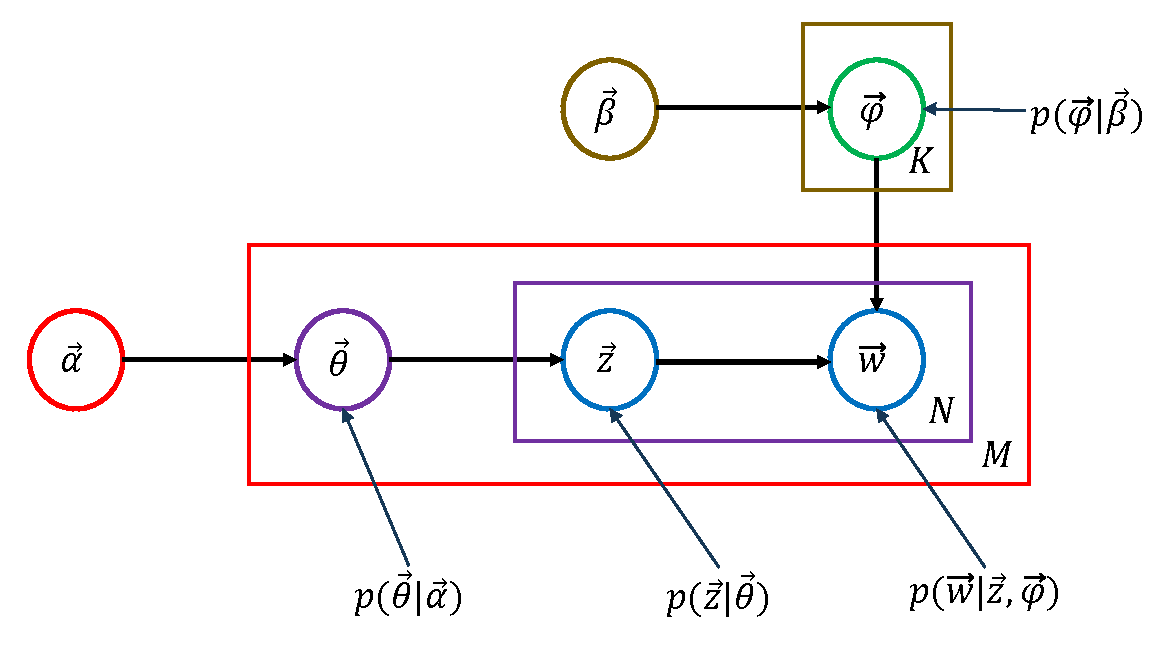
\includegraphics[width = 0.6\textwidth]{LDAFigure}
\end{figure}

整个训练语料库为$\vec{w}$,文档数为$M$,文档$m$中词的个数为$N_m$,则第$m$个文档第$n$词为$w_{m,n}$。
$\vec{w}$的似然函数为:
\begin{displaymath}
\begin{split}
p(\vec{w}|\vec{\alpha}, \vec{\beta}) =
\sum_{\vec{z}}{p(\vec{w}, \vec{z}|\vec{\alpha}, \vec{\beta})}
=\sum_{\vec{z}}{p(\vec{w}|\vec{z},\vec{\beta}) p(\vec{z}|\vec{\alpha})}
\end{split}
\end{displaymath} 

主题数为$K$,词表大小$V$,则主题产生词的概率表$\vec{\phi}$为一个$K
\times V$的一个矩阵,且每个主题($k$)的概率表$\vec{\phi}_k$服从参数为$\vec{\beta}$的Dirichlet
分布:
\begin{displaymath}
\begin{split}
p(\vec{\phi}|\vec{\beta}) &= \prod_{k=1}^{K}{p(\vec{\varphi}_k|\vec{\beta})} 
=\prod_{k=1}^{K}{\frac{\Gamma(\sum_{t=1}^{V}{\beta_t})}{\prod_{t=1}^{V}{\Gamma(\beta_t)}}\prod_{t=1}^{V}{\varphi_{k,t}^{\beta_t-1}}} \\
\end{split}
\end{displaymath} 


给定主题产生词的概率表$\vec{\phi}$以及$M$个文档中所有词的主题编号向量
矩阵$\vec{z}$ (文档数为$M$,文档$m$中词的个数为$N_m$,则第$m$个文档第
$n$词的主题编号为$z_{m,n}$)。矩阵$\vec{z}$跟文档$\vec{w}$是等大小一一
对应的一个矩阵。 $p(\vec{w}|\vec{z},\vec{\phi})$的定义为:
\begin{displaymath}
\begin{split}
p(\vec{w}|\vec{z},\vec{\phi}) 
=\prod_{d=1}^{M}{p(\vec{w}_d|\vec{z}_d, \vec{\phi})} 
=\prod_{d=1}^{M}{\prod_{n=1}^{N_d}{\varphi_{z_{d,n},w_{d,n}}}} 
=\prod_{k=1}^{K}{\prod_{t=1}^{V}{\varphi_{k,t}^{n(k,t)}}}
\end{split}
\end{displaymath}
其中,$\varphi_{z_{d,n},w_{d,n}}$表示第$d$个文档的第$n$个位置的主题
$z_{d,n}$产生词$w_{d,n}$的概率。$n_{k,t}$指的是在所有文档中主题$k$产生
词$t$的次数。

给定$p(\vec{\phi}|\vec{\beta})$和$p(\vec{w}|\vec{z},\vec{\phi})$,则$p(\vec{w}|\vec{z},\vec{\beta})$的定义为:
\begin{displaymath}
\begin{split}
p(\vec{w}|\vec{z},\vec{\beta}) &=
\int{p(\vec{w}|\vec{z},\vec{\phi})p(\vec{\phi}|\vec{\beta})d\vec{\phi}} \\
&= \int{
\prod_{k=1}^{K}{\frac{\Gamma(\sum_{t=1}^{V}{\beta_t})}{\prod_{t=1}^{V}{\Gamma(\beta_t)}}\prod_{t=1}^{V}{\varphi_{k,t}^{\beta_t-1}}}
\cdot
\prod_{k=1}^{K}{\prod_{t=1}^{V}{\varphi_{k,t}^{n(k,t)}}}
d\varphi_{k,t}} \\
&= \int{
\prod_{k=1}^{K}{
    \frac{\Gamma(\sum_{t=1}^{V}{\beta_t})}{\prod_{t=1}^{V}{\Gamma(\beta_t)}}
    \prod_{t=1}^{V}{\varphi_{k,t}^{n(k,t)+\beta_t-1}}
}
d\varphi_{k,t}} \\
&= \int{
\prod_{k=1}^{K}{
    \frac{\triangle(\vec{n}_k+\vec{\beta})}{\triangle(\vec{\beta})}
    \frac{1}{\triangle(\vec{n}_k+\vec{\beta})}
    \prod_{t=1}^{V}{\varphi_{k,t}^{n(k,t)+\beta_t-1}}
}
d\varphi_{k,t}} \Longleftarrow \frac{1}{\triangle(\vec{\beta})}=\frac{\Gamma{(\sum_{t=1}^{V}{\beta_k}})}{\prod_{t=1}^{V}{\Gamma{(\beta_t)}}} \\
&= \prod_{k=1}^{K}{
   \frac{\triangle(\vec{n}_k+\vec{\beta})}{\triangle(\vec{\beta})}
   \underbrace{
   \int{
       \frac{1}{\triangle(\vec{n}_k+\vec{\beta})}
      \prod_{t=1}^{V}{\varphi_{k,t}^{n(k,t)+\beta_t-1}}
    d\varphi_{k,t}}
   }_{\int{Dir(\vec{\varphi}|\vec{n}_k + \vec{\beta})d\vec{\varphi}}=1}
}\\
&= \prod_{k=1}^{K}{ \frac{\triangle(\vec{n}_k+\vec{\beta})}{\triangle(\vec{\beta})}}\\
\end{split}
\end{displaymath} 


文档数为$M$,主题数为$K$,则文档产生主题的概率表$\vec{\theta}$为一个$M
\times K$的矩阵,且第$d$个文档的概率表$\vec{\theta}_d$服从参数为$\vec{\alpha}$的Dirichlet
分布:
\begin{displaymath}
\begin{split}
p(\vec{\theta}|\vec{\alpha}) 
= \prod_{d=1}^{M}{p(\vec{\theta}_d|\vec{\alpha})} 
=\prod_{d=1}^{M}{\frac{\Gamma(\sum_{k=1}^{K}{\alpha_k})}{\prod_{k=1}^{K}{\Gamma(\alpha_k)}}\prod_{k=1}^{K}{\theta_{d,k}^{\alpha_k-1}}} \\
\end{split}
\end{displaymath} 


给定文档产生主题的概率表$\vec{\theta}$, $p(\vec{z}|\vec{\theta})$的定义为:
\begin{displaymath}
\begin{split}
p(\vec{z}|\vec{\theta})
= \prod_{d=1}^{M}{p(\vec{z}_d|\vec{\theta}_d)}
= \prod_{d=1}^{M}{\prod_{n=1}^{N_d}{\theta_{d,z_{d,n}}}}
=\prod_{d=1}^{M}{\prod_{k=1}^{K}{\theta_{d,k}^{n(d,k)}}}
\end{split}
\end{displaymath}
其中,$z_{d,n}$是第$d$个文档第$n$个单词的主题。$\vec{\theta}$中存放
了$d$个文档产生主题$z_{d,n}$的概率$\theta_{d,z_{d,n}}$。$n(d,k)$表示
第$d$个文档中词的主题是$k$的个数。

给定$\vec{\theta}$和$p(\vec{z}|\vec{\theta})$,则$p(\vec{z}|\vec{\alpha})$的定义为:
\begin{displaymath}
\begin{split}
p(\vec{z}|\vec{\alpha}) 
&= \int{p(\vec{z}|\vec{\theta})p(\vec{\theta}|\vec{\alpha})d\vec{\theta}}\\
&= \int{
     \prod_{d=1}^{M}{\frac{\Gamma(\sum_{k=1}^{K}{\alpha_k})}{\prod_{k=1}^{K}{\Gamma(\alpha_k)}}\prod_{k=1}^{K}{\theta_{d,k}^{\alpha_k-1}}}
     \cdot
     \prod_{d=1}^{M}{\prod_{k=1}^{K}{\theta_{d,k}^{n(d,k)}}}
d\vec{\theta}_{d,k}}\\
&= \int{
     \prod_{d=1}^{M}{\frac{\Gamma(\sum_{k=1}^{K}{\alpha_k})}{\prod_{k=1}^{K}{\Gamma(\alpha_k)}}
       \prod_{k=1}^{K}{\theta_{d,k}^{n(d,k)+\alpha_k -1}}
     }
d\vec{\theta}_{d,k}}\\
&= \int{
     \prod_{d=1}^{M}{
       \frac{\triangle(\vec{n}_d+\vec{\alpha})}{\triangle(\vec{\alpha})}
       \frac{1}{\triangle(\vec{n}_d+\vec{\alpha})}
       \prod_{k=1}^{K}{\theta_{d,k}^{n(d,k)+\alpha_k -1}}
     }
d\vec{\theta}_{d,k}}\\
&= \prod_{d=1}^{M}{\frac{\triangle(\vec{n}_d+\vec{\alpha})}{\triangle(\vec{\alpha})}
\underbrace{
    \int{
       \frac{1}{\triangle(\vec{n}_d+\vec{\alpha})}
       \prod_{k=1}^{K}{\theta_{d,k}^{n(d,k)+\alpha_k -1}}
     d\vec{\theta}_{d,k}}
}_{\int{Dir(\vec{\theta}|\vec{n}_d + \vec{\alpha})d\vec{\theta}}=1}
}\\
&= \prod_{d=1}^{M}{\frac{\triangle(\vec{n}_d+\vec{\alpha})}{\triangle(\vec{\alpha})}}\\
\end{split}
\end{displaymath} 

$\vec{w}$的似然函数为:
\begin{displaymath}
\begin{split}
p(\vec{w}|\vec{\alpha}, \vec{\beta}) 
&= \sum_{\vec{z}}{
  p(\vec{w}|\vec{z},\vec{\beta})p(\vec{z}|\vec{\alpha})}\\
&= \sum_{\vec{z}}{(
    \prod_{k=1}^{K}{
        \frac{\triangle(\vec{n}_k+\vec{\beta})}{\triangle(\vec{\beta})}
    }
    \cdot
    \prod_{d=1}^{M}{
        \frac{\triangle(\vec{n}_d+\vec{\alpha})}{\triangle(\vec{\alpha})}
    }
)}\\
&= \sum_{\vec{z}}{(
\prod_{k=1}^{K}{
     {
     \frac{\prod_{t=1}^{V}{\Gamma{((\vec{n}_k+\vec{\beta})_t)}}}{\Gamma{(\sum_{t=1}^{V}{(\vec{n}_k+\vec{\beta})_t})}}
     }
      \cdot
     {
      \frac{\Gamma{(\sum_{t=1}^{V}{\vec{\beta}_t})}}{\prod_{t=1}^{V}{\Gamma{(\vec{\beta}_t)}}}
     }
}
\cdot
\prod_{d=1}^{M}{
     {
      \frac{\prod_{k=1}^{K}{\Gamma((\vec{n}_d+\vec{\alpha})_k)}}{\Gamma(\sum_{k=1}^{K}{(\vec{n}_d+\vec{\alpha})_k}}
     }
\cdot
     { 
      \frac{\Gamma(\sum_{k=1}^{K}{\alpha_k})}{\prod_{k=1}^{K}{\Gamma(\alpha_k)}}
     }
}
)}
\end{split}
\end{displaymath} 
其中,待优化参数为$\vec{n}_k$和$\vec{n}_d$。$\vec{n}_k$是主题$k$产生单
词的计数表,总共有$K$个不同的$\vec{n}_k$,每个$\vec{n}_k$的维度为词表
大小。$\vec{n}_d$是文档$d$产生主题的计数表,总共有$M$个不同的
$\vec{n}_d$,每个$\vec{n}_d$的维度为主题数。


为了能够进行采样,我们需要计算产生第$i=(m,n)$个词(即:第$m$个文档的第
$n$个词)的主题为$k$的条件概
率:$p(z_i=k|\vec{z}_{\neg i}, \vec{w},\vec{\alpha}, \vec{\beta})$.我们定
义如下符号:
$\vec{n}_{k, \neg i}$ 表示将主题为$k$的主题到词的计数$\vec{n}_k$中把第$i$个
词的计数删掉。故而 $(\vec{n}_{k}+\vec{\beta})_i = (\vec{n}_{k, \neg i}+\vec{\beta})_i + 1$,从而有:
\begin{displaymath}
\begin{split}
\frac{\Gamma(\sum_{t=1}^{V}{(\vec{n}_{k, \neg i}+\vec{\beta})_t})  }{ 
       \Gamma(\sum_{t=1}^{V}{(\vec{n}_{k}+\vec{\beta})_t})} 
&= \frac{
     \Gamma(\sum_{t=1; t \neq i}^{V}{(\vec{n}_{k}+\vec{\beta})_t}  
       + (\vec{n}_{k, \neg i}+\vec{\beta})_i)
}{ \Gamma(\sum_{t=1; t \neq i}^{V}{(\vec{n}_{k}+\vec{\beta})_t}
    + (\vec{n}_{k}+\vec{\beta})_i
)} \\
&=  \frac{
     \Gamma(\sum_{t=1; t \neq i}^{V}{(\vec{n}_{k}+\vec{\beta})_t}  
       + (\vec{n}_{k, \neg i}+\vec{\beta})_i)
}{ \Gamma(\sum_{t=1; t \neq i}^{V}{(\vec{n}_{k}+\vec{\beta})_t}
    + (\vec{n}_{k, \neg i}+\vec{\beta})_i +1
)} \\
&=  \frac{1}{\sum_{t=1; t \neq i}^{V}{(\vec{n}_{k}+\vec{\beta})_t}
    + (\vec{n}_{k, \neg i}+\vec{\beta}_i)
} =  \frac{1}{\sum_{t=1}^{V}{(\vec{n}_{k, \neg i}+\vec{\beta})_t}
} \\
\end{split}
\end{displaymath}
同样的$\vec{n}_{m, \neg i}$表示在第$m$个文档中产生词的主题的计数$\vec{n}_m$中把第$i$个
词对应的主题计数删掉。故而 $(\vec{n}_{m}+\vec{\alpha})_k =
(\vec{n}_{m, \neg i}+\vec{\alpha})_k + 1$,从而有:
\begin{displaymath}
\begin{split}
\frac{ \Gamma(\sum_{k'=1}^{K}{(\vec{n}_{m, \neg i}+\vec{\alpha})_{k'}})
}{     \Gamma(\sum_{k'=1}^{K}{(\vec{n}_{m}+\vec{\alpha})_{k'}}) 
}
&=  \frac{1}{\sum_{k'=1}^{K}{(\vec{n}_{m, \neg i}+\vec{\alpha})_{k'}}
} \\
\end{split}
\end{displaymath}

$p(\vec{w}_{\neg i}| \vec{z_{\neg i}}, \vec{\alpha},\vec{\beta})$ 和
$p(\vec{z}_{\neg i}|\vec{\alpha}, \vec{\beta})$ 表示将第$i=(m,n)$个词
删掉,从而产生一个新的语料。新的语料同原始语料的区别仅仅在于第$m$个文
档中不包含第$n$个词,故而其产生过程中也不需要生成对应的$z_i$。我们记第
$i$个term 的 ID为$t$,第$i$个词的主题为$k$。
\begin{displaymath}
\begin{split}
p(\vec{w}_{\neg i}| \vec{z_{\neg i}}, \vec{\beta}) &= 
\prod_{k'=1;k' \neq k}^{K}{
       \frac{\triangle(\vec{n}_{k'}+\vec{\beta})}
            {\triangle(\vec{\beta})}})
\cdot
 \frac{\triangle(\vec{n}_{k, \neg i}+\vec{\beta})}
      {\triangle(\vec{\beta})}\\
p(\vec{z}_{\neg i}|\vec{\alpha}) &=
\prod_{d=1; d \neq m}^{M}{\frac{\triangle(\vec{n}_d+\vec{\alpha})}
                  {\triangle(\vec{\alpha})}}
       \cdot
\frac{\triangle(\vec{n}_{m; \neg i}+\vec{\alpha})}
     {\triangle(\vec{\alpha})}
\end{split}
\end{displaymath}

\begin{displaymath}
\begin{split}
p(z_i=k|\vec{z}_{\neg i}, \vec{w}, \vec{\alpha}, \vec{\beta}) &=
\frac{ p(\vec{w}, \vec{z}|\vec{\alpha}, \vec{\beta}) }
     { p(\vec{w}, \vec{z_{\neg i}}|\vec{\alpha}, \vec{\beta})}\\
&=\frac{ p(\vec{w}| \vec{z}, \vec{\alpha}, \vec{\beta})
         p(\vec{z}| \vec{\alpha}, \vec{\beta})  }
     { p(\vec{w}_{\neg i}| \vec{z_{\neg i}},\vec{\alpha},\vec{\beta})
        p(\vec{z_{\neg i}}|\vec{\alpha},\vec{\beta})
      p(w_i|\vec{z}_{\neg i}, \vec{\alpha}, \vec{\beta})} \\
&= \frac{ p(\vec{w}| \vec{z}, \vec{\beta}) }
     { p(\vec{w}_{\neg i}| \vec{z_{\neg i}}, \vec{\beta})p(w_i|\vec{\alpha}, \vec{\beta})}
\cdot
\frac{p(\vec{z}|\vec{\alpha})}{p(\vec{z}_{\neg
    i}|\vec{\alpha})}
\\
&\propto  \frac{ p(\vec{w}| \vec{z}, \vec{\beta}) }
     { p(\vec{w}_{\neg i}| \vec{z_{\neg i}}, \vec{\beta})}
\cdot
\frac{p(\vec{z}|\vec{\alpha})}{p(\vec{z}_{\neg i}|\vec{\alpha})}
\Longleftarrow p(w_i|\vec{\alpha}, \vec{\beta})=C
\\
&=  \frac{
      \prod_{k'=1}^{K}{\frac{\triangle(\vec{n}_{k'}+\vec{\beta})}
                   {\triangle(\vec{\beta})}} 
    }
     {(\prod_{k'=1;k' \neq k}^{K}{
       \frac{\triangle(\vec{n}_{k'}+\vec{\beta})}
            {\triangle(\vec{\beta})}})
      \cdot
       \frac{\triangle(\vec{n}_{k, \neg i}+\vec{\beta})}
            {\triangle(\vec{\beta})}
      }
\cdot
\frac{
     \prod_{d=1}^{M}{\frac{\triangle(\vec{n}_d+\vec{\alpha})}
                  {\triangle(\vec{\alpha})}}
     }{
       \prod_{d=1; d \neq m}^{M}{\frac{\triangle(\vec{n}_d+\vec{\alpha})}
                  {\triangle(\vec{\alpha})}}
       \cdot
       \frac{\triangle(\vec{n}_{m; \neg i}+\vec{\alpha})}
            {\triangle(\vec{\alpha})}
}\\
&= \frac{ \triangle(\vec{n}_{k}+\vec{\beta}) }
        { \triangle(\vec{n}_{k, \neg i}+\vec{\beta})
        }
\cdot
\frac{\triangle(\vec{n}_{m}+\vec{\alpha})
     }{\triangle(\vec{n}_{m; \neg i}+\vec{\alpha})
}\\
&= \frac{\Gamma(\sum_{t'=1}^{V}{(\vec{n}_{k, \neg i}+\vec{\beta})_{t'}})
        \cdot
        \prod_{t'=1}^{V}{ \Gamma((\vec{n}_{k}+\vec{\beta})_{t'}) }
        }{
       \prod_{t'=1}^{V}{ \Gamma((\vec{n}_{k, \neg i}+\vec{\beta})_{t'}) }
       \cdot
       \Gamma(\sum_{t'=1}^{V}{(\vec{n}_{k}+\vec{\beta})_{t'}})
}\\
&\cdot
\frac{ \Gamma(\sum_{k'=1}^{K}{(\vec{n}_{m, \neg i}+\vec{\alpha})_{k'}})
       \cdot
        \prod_{k'=1}^{K}{ \Gamma(\vec{n}_{m}+\vec{\alpha})_{k'} }
}{     \Gamma(\sum_{k'=1}^{K}{(\vec{n}_{m}+\vec{\alpha})_{k'}})
        \cdot
       \prod_{k'=1}^{K}{ \Gamma(\vec{n}_{m, \neg i}+\vec{\alpha})_{k'} }
}\\
&= \frac{\prod_{t'=1}^{V}{  \Gamma((\vec{n}_{k}+\vec{\beta})_{t'})  }
        }{
       \prod_{t'=1}^{V}{ \Gamma((\vec{n}_{k, \neg i}+\vec{\beta})_{t'}) }
       \cdot
       \sum_{t'=1}^{V}{(\vec{n}_{k, \neg i}+\vec{\beta})_{t'}}
       }\\
&\cdot
\frac{ \prod_{k'=1}^{K}{ \Gamma(\vec{n}_{m}+\vec{\alpha})_{k'}}
}{     \prod_{k'=1}^{K}{ \Gamma(\vec{n}_{m, \neg i}+\vec{\alpha})_{k'}}
        \cdot
        \sum_{k'=1}^{K}{(\vec{n}_{k', \neg i}+\vec{\alpha})_{k'}}
}\\
&= \frac{\Gamma((\vec{n}_{k}+\vec{\beta})_t)
        }{
       \Gamma((\vec{n}_{k, \neg i}+\vec{\beta})_t)
       \cdot
       \sum_{t'=1}^{V}{(\vec{n}_{k, \neg i}+\vec{\beta})_{t'}}
       }\\
&\cdot
\frac{\Gamma((\vec{n}_{m}+\vec{\alpha})_{k})
}{ \Gamma((\vec{n}_{m, \neg i}+\vec{\alpha})_{k})
        \cdot
        \sum_{k'=1}^{K}{(\vec{n}_{k', \neg i}+\vec{\alpha})_{k'}}
}\\
&= \frac{(\vec{n}_{k, \neg i}+\vec{\beta})_t
        }{
       \sum_{t'=1}^{V}{(\vec{n}_{k, \neg i}+\vec{\beta})_{t'}}
       }
\cdot
\frac{((\vec{n}_{m, \neg i}+\vec{\alpha})_{k}
}{\sum_{k'=1}^{K}{(\vec{n}_{k', \neg i}+\vec{\alpha})_{k'}}
}\\
\end{split}
\end{displaymath}

由Dirichlet分布的期望公式得:
\begin{displaymath}
\begin{split}
 \hat{\varphi}_{kt} &= \frac{(\vec{n}_{k, \neg i}+\vec{\beta})_t
        }{
       \sum_{t'=1}^{V}{(\vec{n}_{k, \neg i}+\vec{\beta})_{t'}}
       }
\\
\hat{\theta}_{mk} &= \frac{((\vec{n}_{m, \neg i}+\vec{\alpha})_{k}
}{\sum_{k'=1}^{K}{(\vec{n}_{k', \neg i}+\vec{\alpha})_{k'}}
}
\end{split}
\end{displaymath}

给定$\vec{\alpha}$作为先验,我们使用模型来产生了一批数据,这批数
据除了没有产生第$m$个文档的第$n$个词,其余同原始数据一样,即
$\vec{z}_{\neg i}$以及$\vec{w}_{\neg i}$,那么$\vec{\theta}_m$
的后验概率仍然为一个$Dir$概率分布,故而有$p(\vec{\theta}_m|\vec{z}_{\neg i}, \vec{w}_{\neg i}) = Dir(\vec{\theta}_m|\vec{n}_{m, \neg i} + \vec{\alpha})$。同理
$p(\vec{\varphi}_k|\vec{z}_{\neg i}, \vec{w}_{\neg i}) =
Dir(\vec{\varphi}_k|\vec{n}_{k, \neg i}+\vec{\beta})$。基于这两个公式,
我们可以用另一个方法进行证明:
\begin{displaymath}
\begin{split}\
p(z_i=k|\vec{z}_{\neg i}, \vec{w})  
&= p(z_i=k|\vec{z}_{\neg i},w_i=t, \vec{w}_{\neg i})  \\
&=\frac{p(z_i=k, w_i=t|\vec{z}_{\neg i}, \vec{w}_{\neg i})}{p(w_i = t)}\\
&\propto
p(z_i=k,w_i=t|\vec{z}_{\neg i}, \vec{w}_{\neg i})\\
&=\int{p(z_i=k, w_i=t, \vec{\theta}_m, \vec{\varphi}_k|\vec{z}_{\neg i},
\vec{w}_{\neg i})}d\vec{\theta}_md\vec{\varphi}_k\\
&=\int{p(z_i=k, \vec{\theta}_m|\vec{z}_{\neg i},
\vec{w}_{\neg i})
p(w_i=t, \vec{\varphi}_k|\vec{z}_{\neg i},
\vec{w}_{\neg i})}d\vec{\theta}_md\vec{\varphi}_k\\
&=\int{p(z_i=k|\vec{\theta}_m)
p(\vec{\theta}_m|\vec{z}_{\neg i}, \vec{w}_{\neg i})
p(w_i=t| \vec{\varphi}_k)
p(\vec{\varphi}_k|\vec{z}_{\neg i}, \vec{w}_{\neg i})
}d\vec{\theta}_md\vec{\varphi}_k\\
&=\int{p(z_i=k|\vec{\theta}_m)
p(\vec{\theta}_m|\vec{z}_{\neg i}, \vec{w}_{\neg i})
}d\vec{\theta}_m
\int{p(w_i=t| \vec{\varphi}_k)
p(\vec{\varphi}_k|\vec{z}_{\neg i}, \vec{w}_{\neg i})
}d\vec{\varphi}_k\\
&=\int{p(z_i=k|\vec{\theta}_m)
Dir(\vec{\theta}_m|\vec{n}_{m, \neg i} + \vec{\alpha})
}d\vec{\theta}_m 
 \cdot \int{
p(w_i=t| \vec{\varphi}_k)
Dir(\vec{\varphi}_k|\vec{n}_{k, \neg i}+\vec{\beta})
}d\vec{\varphi}_k\\
&=\int{\theta_{mk}
Dir(\vec{\theta}_m|\vec{n}_{m, \neg i} + \vec{\alpha})
}d\vec{\theta}_m  \cdot \int{
\varphi_{kt}
Dir(\vec{\varphi}_k|\vec{n}_{k, \neg i}+\vec{\beta})
}d\vec{\varphi}_k\\
&= \mathbf{E}(\theta_{mk}) \cdot \mathbf{E}(\varphi_{kt})\\
&= \hat{\theta}_{mk} \cdot \hat{\varphi}_{kt}
\end{split}
\end{displaymath}


\begin{minipage}{0.8\textwidth}\centering
\begin{algorithm}[H]
$\boxdot$ initialization:\\
zero all count variables, $n_m^{(k)}$, $n_m$, $n_k^{(t)}$, $n_k$\\
\For{all documents $m \in [1,M]$}{
  \For{all words $n \in [1, N_m]$ in document $m$}{
      sample topic index $z_{m,n}=k \sim Mult(1/K)$\\
      increment document-topic count:$n_m^{(k)}+1$\\
      increment document-topic sum: $n_m + 1$\\
      increment topic-term count: $n_k^{(t)}+1$\\
      increment topic-term sum: $n_k+1$\\
  }
}
$\boxdot$ Gibbs sampling over burn-in period and sampling period:\\
\While{not finished}
{
  \For{all documents $m \in [1,M]$}{
    \For{all words $n \in [1, N_m]$ in document $m$}{
      $\boxdot$ for the current assignment of $k$ to a term $t$ for word $w_{m,n}$:\\
      decrement counts and sums: $n_m^{(k)}-1$, $n_m-1$, $n_k^{(t)}-1$,
      $n_k-1$;\\
      $\boxdot$ multinomial sampling (decrements from previous step):\\
      sample topic index $\tilde{k} \sim p(z_i|\vec{z}_{\neg i}, \vec{w})$;\\
      $\boxdot$ use the new assignment of $z_{m,n}$ to the term $t$ for word
      $w_{m,n}$:\\
      increment counts and sums: $n_m^{(\tilde{k})}-1$, $n_m-1$, $n_{\tilde{k}}^{(t)}-1$, $n_{\tilde{k}}-1$;
    }
  }
   $\boxdot$ Check convergence and read out parameters:\\
   \If{converged and $L$ sampling iterations since last read out}
   {
      $\boxdot$ the different parameters read outs are averaged:\\
      read out parameters set $\vec{\phi}$\\
      read out parameters set $\vec{\theta}$
  }
}
\end{algorithm}
\end{minipage}


% !Mode:: "TeX:UTF-8"

\chapter{随机过程}

\section{高斯过程(Gaussian Process)}
\subsection{从K最近邻说起}
如图所示,建设我们有一批二维带标记的数据,给定一个新的样本,我们需要判断该样本的标记。K最近邻的思想非常简单,我们可以选择K个距离该样本最近的有标记的样本,然后根据这K个最相似的样本来推断新样本的标记。这是一个最简单也是最有效的方法,数据即模型,这类方法称为memory-based方法。

\begin{center}
\begin{tikzpicture}[scale=1.0]
\node[mark size=3pt, color=blue] at (-1, 3) {\pgfuseplotmark{triangle*}};
\node[mark size=3pt, color=blue] at (-1, 2) {\pgfuseplotmark{triangle*}};
\node[mark size=3pt, color=blue] at (-1, 1) {\pgfuseplotmark{triangle*}};
\node[mark size=3pt, color=blue] at (-0.5, 1.5) {\pgfuseplotmark{triangle*}};
\node[mark size=3pt, color=blue] at (0, 2.5) {\pgfuseplotmark{triangle*}};
\node[mark size=3pt, color=blue] at (1, 1.2) {\pgfuseplotmark{triangle*}};

\node[mark size=3pt, color=red] at (-1, 1) {\pgfuseplotmark{*}};
\node[mark size=3pt, color=red] at (1, 1.5) {\pgfuseplotmark{*}};
\node[mark size=3pt, color=red] at (1, 2.3) {\pgfuseplotmark{*}};
\node[mark size=3pt, color=red] at (0.5, 2.5) {\pgfuseplotmark{*}};
\node[mark size=3pt, color=red] at (1.5, 2.15) {\pgfuseplotmark{*}};

\node[mark size=3pt, color=green] at (1, 2) {\pgfuseplotmark{square*}};

\draw (1,2) circle (0.5cm);
\draw[dashed] (1,2) circle (1cm);
\draw[dashed] (1,2) circle (1.5cm);
\end{tikzpicture}
\end{center}

K最近邻一般是用来做分类,如果我们用K最近邻来做回归呢?如下图,我们有三个有标注的数据,分别为$(x_1, f_1), (x_2, f_2), (x_3, f_3)$,那么我们如何预测一个新给的样本$x^*$的值$f^*$呢,我们同样也可以选择K个离$x^*$最近的训练数据,然后根据距离加权得到值$f^*$,或者我们可以使用所有的训练数据来计算$f^*$。

\begin{center}
\begin{tikzpicture}[scale=1.0]
\draw [<->, thick] (0,4) node (yaxis) [above] {$y$} |- (5,0) node (xaxis) [right] {$x$};
\draw[blue, dashed] (0, 3.5) node (f3) [left]{$f_3$} |- (4, 3.5);
\draw[blue, dashed] (4, 3.5) |- (4,0) node (x3) [below]{$x_3$};
\fill[blue] (4, 3.5) circle(2pt);

\draw[blue, dashed] (0,2.3) node (f2) [left]{$f_2$} |- (2.1,2.3);
\draw[blue, dashed] (2.1,2.3) |- (2.1,0) node (x2) [below]{$x_2$};
\fill[blue] (2.1,2.3) circle(2pt);

\draw[blue, dashed] (0,1.2) node (f1) [left]{$f_1$} |- (1.5,1.2);
\draw[blue, dashed] (1.5,1.2) |- (1.5,0) node (x1) [below]{$x_1$};
\fill[blue] (1.5,1.2) circle(2pt);

\draw[red, dashed] (0,3) node (f1) [left]{$f^*$} |- (3,3);
\draw[red, dashed] (3,3) |- (3,0) node (x1) [below]{$x^*$};
\fill[red] (3,3) circle(2pt);
\end{tikzpicture}
\end{center}

\subsection{高斯过程回归}

高斯过程指的是一组随机变量的集合,这个集合中任意的有限个随机变量都服从联合高斯分布。形式化的有:
\begin{displaymath}
\begin{split}
\begin{bmatrix}
f_1\\
f_2\\
f_3\\
\end{bmatrix}
\sim \mathcal{N} \left(
\begin{bmatrix}
0\\
0\\
0\\
\end{bmatrix},
\begin{bmatrix}
k_{11} & k_{12} & k_{13}\\
k_{21} & k_{22} & k_{23}\\
k_{31} & k_{32} & k_{33}\\
\end{bmatrix}
\right)
\end{split}
\end{displaymath}

对上边提到的回归问题,我们假设这些$f$值服从联合高斯分布,那么这个联合高斯分布的协方差$\mathcal{K}$如何获得?我们知道该联合高斯分布的协方差$\mathcal{K}$描述了样本的$f$值之间的相关程度。 在K近邻模型里面,我们有这样的假设,即如果样本的距离越近其$f$值越相关(回归函数是平滑的)。那么协方差$\mathcal{K}$便可以用样本的距离(相似度)来代替。那么如何使用样本的距离来计算协方差矩阵(半正定矩阵)呢?核函数。
比如我们可以定义协方差矩阵为高斯核(RBF kernel or squared exponential kernel):
\begin{displaymath}
\begin{split}
\mathcal{K}_{ij} = e^{-\lambda \| x_i-x_j \|^2}
\end{split}
\end{displaymath}
很明显当$\| x_i-x_j \|$无穷大时$\mathcal{K}_{ij}$为0, 当$\| x_i-x_j \|$为0时,$\mathcal{K}_{ij}$为1。

那么回到原来的回归问题,给定了三个样本$(x_1, f_1), (x_2, f_2), (x_3, f_3)$,我们使用高斯过程来预测一个新给的样本$x^*$的值$f^*$:
\begin{displaymath}
\begin{split}
\begin{bmatrix}
f_1\\
f_2\\
f_3\\
f^*\\
\end{bmatrix}
\sim \mathcal{N} \left(
\begin{bmatrix}
0\\
0\\
0\\
0\\
\end{bmatrix},
\begin{bmatrix}
k_{11} & k_{12} & k_{13} & k_{1*}\\
k_{21} & k_{22} & k_{23} & k_{2*}\\
k_{31} & k_{32} & k_{33} & k_{3*}\\
k_{*1} & k_{*2} & k_{*3} & k_{**}\\
\end{bmatrix}
\right)
\end{split}
\end{displaymath}

由于我们已经有了$f_1, f_2, f_3, f^*$的联合分布,故可得$f^*$的条件分布为$f^* \sim \mathcal{N}(\mu^*, \sigma^*)$,其中$\mu^* = k_*^T k^{-1} \vec{f}, \sigma^*= -k_*^Tk^{-1}k_* + k_{**}$,即:
\begin{displaymath}
\begin{split}
p(f^*) &= \frac{1}{\sqrt{2\pi}\sigma^*} \exp{\left ( - \frac{(x-\mu^*)^2}{2{\sigma^*}^2} \right)}\\
&= \frac{1}{\sqrt{2\pi} (-k_*^Tk^{-1}k_* + k_{**})} \exp{\left ( - \frac{(x-  k_*^T k^{-1} \vec{f})^2}{2{(-k_*^Tk^{-1}k_* + k_{**})}^2} \right)}\\
\end{split}
\end{displaymath}

当给定$x^*$,我们根据该分布便可以采样一个对应的$f^*$,使用Reparameterization Trick,我们可以将该采样过程等价为:
\begin{displaymath}
\begin{split}
\varepsilon \sim & \mathcal{N}(0, 1)\\
f^* = & \mu^* + \varepsilon \sigma^* \\
 =&  k_*^T k^{-1} \vec{f} + \varepsilon ( -k_*^Tk^{-1}k_* + k_{**})\\
\end{split}
\end{displaymath}
换言之,我们可以直接采样一个函数,即,$p(f^*)$本质上是函数$f$的概率分布,是一个函数的函数。

\begin{figure}[htbp]
\centering
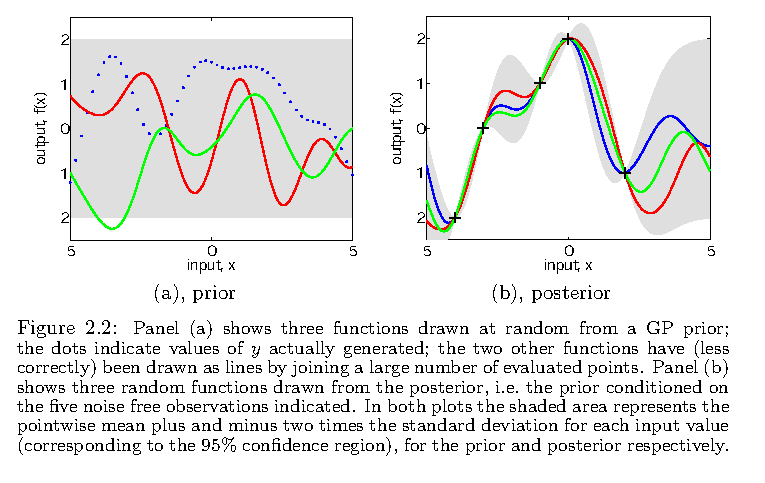
\includegraphics[width = 0.8\textwidth]{GPRegression}
\end{figure}

\section{狄利克雷过程(Dirichlet Process)}


\subsection{从有限混合到无限混合}

我们可以从一个聚类的任务来看一下为什么说狄利克雷过程是狄利克雷混合在类别是无限时候的一个扩展。
给定数据$X=(x_0, x_1, ...)$,我们首先假设数据应该聚成$K$类,每一类服从一个高斯分布。从这个$K$个类别中选择一类,并产生一个样本的概率服从多项式分布$p(Z|\pi)=\prod_{k=1}^{K} \pi_k^{m_k}$,其中$\pi_k$表示选择第$k$类的概率,而$m_k$表示$X$的所有样本中,从第$k$个类中产生的总的数量。而这个多项式分布的参数$\pi$服从一个以$\alpha$为参数的狄利克雷先验,我们假设每个高斯分布的均值$\mu_k$服从一个以$\lambda$为参数的基础分布$H(\lambda)$, 即:
\begin{displaymath}
\begin{split}
(x_i|z_i=k, \mu_k) \sim & N(\mu_k, \sigma^2)\\
p(z_i=k) = & \pi_k\\
(\boldsymbol{\pi}|\alpha) \sim &Dir(\frac{\alpha}{K} . \mathrm{1}_{K} )\\
\mu_k \sim & H(\lambda)
\end{split}
\end{displaymath}
为了同DP进行比较我们将上边的模型重写为:
\begin{displaymath}
\begin{split}
(x_i|\tilde{\mu}_i) \sim & N(\tilde{\mu}_i, \sigma^2)\\
\tilde{\mu}_i \sim & G=\sum_{k=1}^{K}\pi_k\delta_{\mu_k}(\tilde{\mu}_i) \\
(\boldsymbol{\pi}|\alpha) \sim &Dir(\frac{\alpha}{K} . \mathrm{1}_{K} )\\
\mu_k \sim & H(\lambda)
\end{split}
\end{displaymath}
其中$\delta_{x}$为指示函数,$\delta_{x}(x)=1$,否则为0。即,$G$是一个离散分布,只有点$\mu_k, k=1,2,...,K$上有密度,其它位置概率密度为0。在新的改写后的模型中,我们假设每个样本都是从高斯分布中采样得到的,每个高斯分布的均值$\tilde{\mu}_i$服从离散的概率分布$G$。$G$是一个特殊的概率分布,只在$K$个位置($\mu_k, k=1,2,...,K$)上概率密度不为零,而这$K$个位置则独立同分布于一个基础分布$H(\lambda)$。每个位置点上的概率密度$\pi_k, k=1,2,...,K$服从狄利克雷分布$Dir(\frac{\alpha}{K} . \mathrm{1}_{K})$。

如果我们事先并不知道到底应该聚成几类呢,即$\tilde{\mu}_i$是从一个可能有无穷个点的离散分布中采样的:$\tilde{\mu}_i \sim G=\sum_{k=1}^{\infty}\pi_k\delta_{\mu_k}(\tilde{\mu}_i)$。那么,这样的一个$G$就是一个狄利克雷过程。
\begin{displaymath}
\begin{split}
(x_i|\tilde{\mu}_i) \sim & N(\tilde{\mu}_i, \sigma^2)\\
\tilde{\mu}_i \sim & G=\sum_{k=1}^{\infty}\pi_k\delta_{\mu_k}(\tilde{\mu}_i) \\
G \sim & DP(H(\lambda), \alpha)\\
\end{split}
\end{displaymath}

我们用$\mathbf{z}_{n,-i}$表示FMM中第$k$个聚类中去掉第$i$个节点的,那么
\begin{displaymath}
\begin{split}
p(z_i=k|\mathbf{z}_{n,-i}, \alpha) &= \frac{n_{k,-i} + \alpha/K}{n+\alpha-1}\\
\end{split}
\end{displaymath}
$K$趋向于无穷大时,当$n_{k,-i} > 0$时:
\begin{displaymath}
p(z_i=k|\mathbf{z}_{n,-i}, \alpha) = \frac{n_{k,-i}}{n+\alpha-1}
\end{displaymath}
对于其它的样本数为0的类别:
\begin{displaymath}
p(z_i \neq z_j ~~for~~all~~j \neq i|\mathbf{z}_{n,-i}, \alpha) = \frac{\alpha}{n+\alpha-1}
\end{displaymath}

\subsection{Dirichlet Process}

\textbf{Dirichlet Distribution}: 我们有一张纸,纸上列了$K$中不同的颜色,我们在大街上随机的找一个行人,问他喜欢那种颜色,并将对应颜色数+1。当我们采访的次数趋向于无穷时,颜色的分布是一个狄利克雷分布。

\textbf{Dirichlet Process}: 我们有一张纸,纸上是空白的,我们在大街上随机的找一个行人,问他喜欢那种颜色,行人可以从已经写在纸上的颜色选一个,也可以自己提一个颜色(这样可能的颜色数量就是无穷的),并将其写在纸上,我们将对应颜色数+1。当我们采访的次数趋向于无穷时,颜色的分布是一个狄利克雷过程分布。

狄利克雷分布和狄利克雷过程都可以对一个符号流进行建模,不同的是,狄利克里分布要求符号表是给定的有限的,而狄利克雷过程的符号表可能是无限的。假设我们目前观测到的符号流的长度为$F$,每个符号用一个独一无二的正整数表示$w \in [0, \infty)$,并且用$F_w$表示符号$w$已经出现过的次数,狄利克雷过程表示如下的一个分布:1),下一个符号是已知符号$w$的概率为$\frac{F_w}{F+\alpha}$;2),下一个符号是一个新符号的概率是$\frac{\alpha}{F+\alpha}$。

我们称分布$G$是一个以$G_0$和$\alpha$为参数的狄利克雷过程$G \sim DP(G_0, \alpha)$,其中$G_0$为基础分布,$\alpha$为度量集中性的一个参数。狄利克雷过程是狄利克雷分布向符号表为无穷时的一个扩展。
\begin{figure}[htbp]
\centering
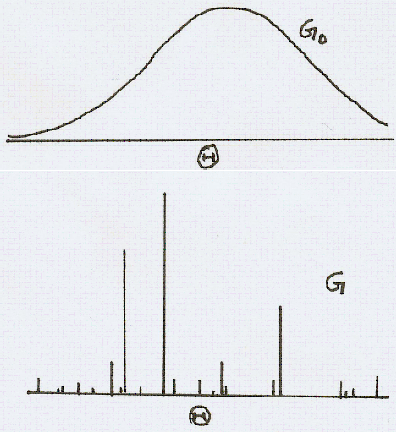
\includegraphics[width = 0.4\textwidth]{DirichletProcess0}
\end{figure}

\textbf{Motivation},当我们对数据$X=(x_0, x_1, ...)$聚类时,我们事先并不知道这些数据到底应该聚成多少类。我们只能假设这些数据是从某些参数为$\theta_{c}$的分布$P_{\theta_c}$中采样出来的,从同一个分布(相同的参数$\theta_c$)采样出来的数据属于同一类。我们又假设这些参数$\theta_c$服从某个连续分布$H$。我们可以按照这样的思路来进行采样,从$H$中采样一个$\theta_c$,并从分布$P_{\theta_c}$中采样一个样本。然而这样的过程是有问题的,因为参数$\theta_c$是连续值,那么从连续分布$H$中采样两个相等的连续值的概率为0。那么我们需要找一个离散分布$G$,希望该离散分布$G$能够同$H$足够的相似。狄利克雷过程就是这些离散分布$G$的一个分布,我们可以从$DP(H,\alpha)$中采样这样的一个$G$。
采样得到的$G$是一个由随机的支持点$\theta_c$和对应的权重$w_c$构成,如下:

\begin{displaymath}
\begin{split}
G&=\sum_{c=1}^{\infty}w_c\delta_{\theta_c}\\
w &\sim Stick(\alpha)\\
\theta_c &\overset{iid}{\sim}H
\end{split}
\end{displaymath}
其中$\sum_{c=1}^{\infty}w_c=1$.并且Stick-breaking的权重$w_c$通过如下方式产生:
\begin{displaymath}
\begin{split}
w_c = v_c \prod_{l=1}^{c-1}(1-v_l),~~where~~v_c \overset{iid}{\sim} Beta(1,\alpha)
\end{split}
\end{displaymath}
如此,则基础分布$H$决定了支持点$\theta_c$(概率密度不为0的点)的位置,而stick-breaking的权重决定了每个类别的量(支持点的概率密度)。

当$\alpha \to 0$时,第一个权重的采样将接近于1,在这种情况下,随机采样得到的$G$会有一个单独的支持点,并且每次采样得到的$G$均会不同,因为每次的支持点将会不同。当$\alpha \to \infty$时,权重的采样就会集中在非常小的数值上,从而会有非常多的不同的支持点,$G$将会无限接近$H$。参数$\alpha$便是用来控制$G$和$H$的相似程度。

\begin{figure}[htbp]
\centering
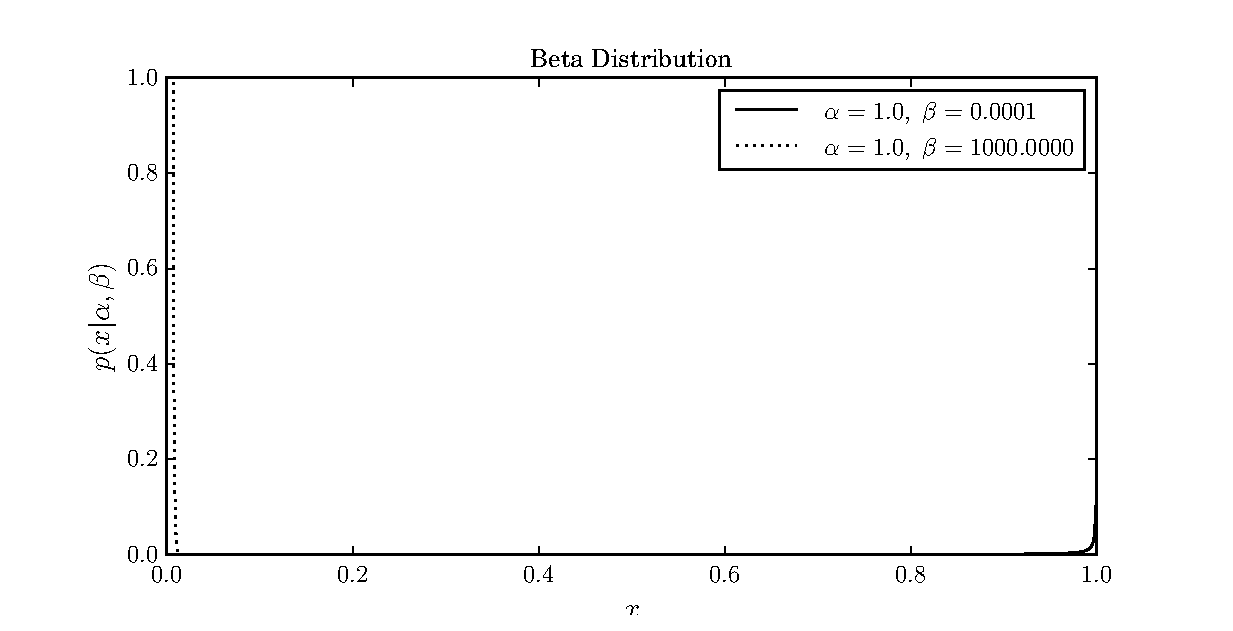
\includegraphics[width = 0.9\textwidth]{BetaDistribution2}
\end{figure}

\begin{figure}[htbp]
\centering
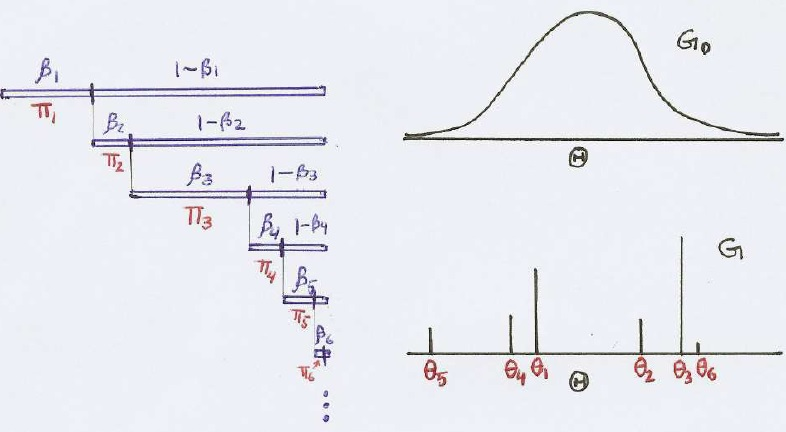
\includegraphics[width = 0.9\textwidth]{StickBreakingProcess}
\end{figure}

\textbf{Defination of Dirichlet Process}:给定一个测度空间$\Omega$,一个基础分布$H$,一个正实数$\alpha$,那么狄利克雷过程$Dir(H, \alpha)$是一个随机过程(即,分布的分布),该随机过程的采样$G$是$S$上的一个概率分布,并且对于$\Omega$的任意一个划分$\{B_i\}_{i=1}^{n}$,$G$满足如下条件:
\begin{displaymath}
\begin{split}
(G(B_1),...,G(B_n)) \sim Dir(\alpha H(B_1),...,\alpha H(B_n))
\end{split}
\end{displaymath}
其中:$G(B_i)=\int_{B_i} \mathrm{d} G, H(B_i) = \int_{B_i} \mathrm{d} H$。

\textbf{Stick-Breaking Process}

假设我们有一个长度为1的棍子,我们令$\beta_c \sim Beta(1, \alpha), c=1,2,3,....$为我们每次从剩下的棍子上折下来的比例,$\pi_c$为我们每次折下来的长度:
\begin{displaymath}
\begin{split}
\pi_1= \beta_1, \pi_2=(1-\beta_1)\beta_2, ...., \pi_c=\beta_c\prod_{j=1}^{c-1}(1-\beta_j),...
\end{split}
\end{displaymath}
即构造过程如下:

\begin{minipage}{0.8\textwidth}\centering
\begin{algorithm}[H]
\textbf{Stick-Breaking Process}($H, \alpha$):\\
\For{c=0,1,...}{
Sample $\beta_c$ from $Beta(1,\alpha)$;\\
$\pi_c=\beta_c\prod_{j=1}^{c-1}(1-\beta_j)$;\\
Sample $\theta_c$ from base distribution $H$;\\
}
$G=\sum_{c=1}^{\infty}\pi_c\delta_{\theta_c}$;//means $(\pi_c, \theta_c)$ is a sample from $DP(H,\alpha)$
\end{algorithm}
\end{minipage}


\textbf{Polya Urn Scheme}
同Polya Urn做狄利克雷分布采样类似,我们可以用桶和球来做狄利克雷过程的采样。我们从一个空的桶开始(狄利克雷分布是从一个已有若干个球的桶开始),我们以两种形式往桶里添加球:1)以概率$\frac{\alpha}{\alpha+n-1}$的概率从基础分布$H$中采样一个颜色$\theta_k$,并将一个新的球涂成该颜色放入桶中;2)从桶中随机拿出一个球,并涂一个新的球为该拿出球的颜色,并将这两个球一并放入桶中。假设桶中已有$K$中颜色,每种颜色的球的个数为$n_k$,那么第二种方式相当于以概率$\frac{n_k}{\alpha+n-1}$往桶中添加一个第$k$中颜色的球。综上,给定前$n-1$个球的颜色$\phi_{1:n-1}$,第$n$个球的颜色$\phi_n$服从如下分布:

\begin{displaymath}
\begin{split}
\phi_n | \phi_{1:n-1} \sim \frac{\alpha G_0(\phi_n)}{\alpha+n-1} + \frac{\sum_{j=1}^{n-1} \delta(\phi_n-\phi_j) }{\alpha+n-1}
\end{split}
\end{displaymath}
其中$\delta(0)=1$,其余值为0。

\textbf{Chinese Restaurant Process}

假设有一家中国餐馆,里边有无数的桌子。第一个进来的顾客坐了第一张桌子。后边进来的第$n$个顾客服从下边的规则来选择桌子:1),以概率$\frac{n_k}{\alpha  + n -1}$选择第$k$张桌子,其中$n_k$为第$k$张桌子已有的顾客数;2),以概率$\frac{\alpha  }{\alpha   + n -1}$新开一张桌子。

\begin{figure}[htbp]
\centering
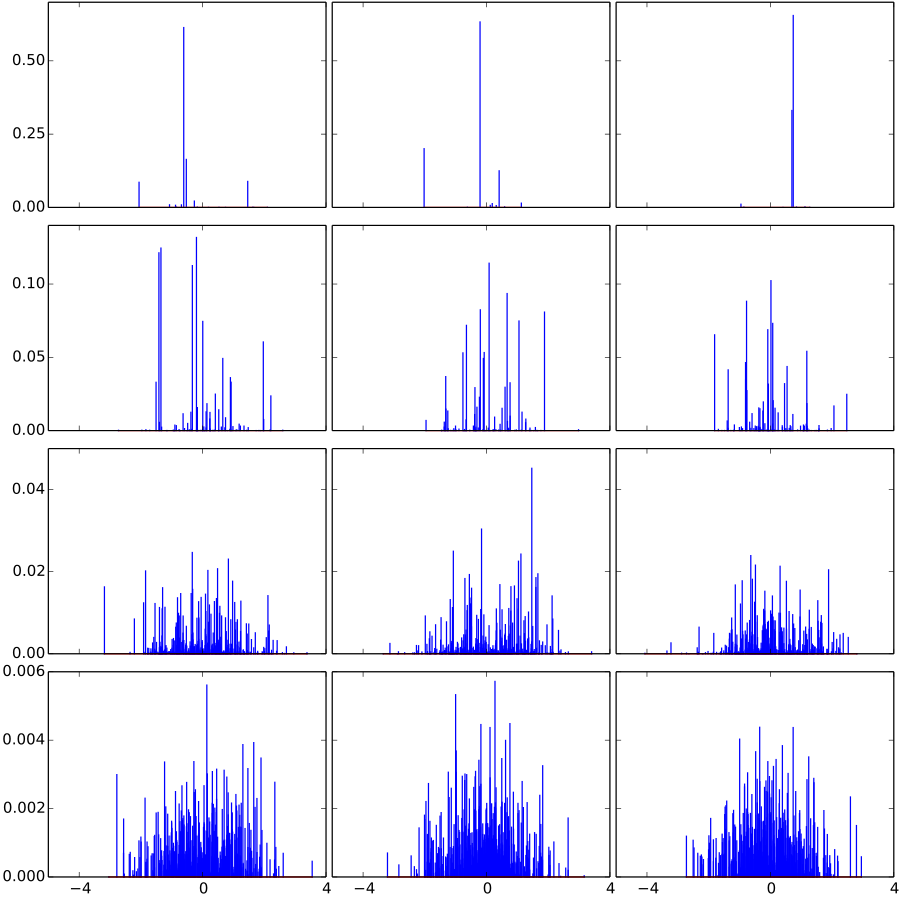
\includegraphics[width = 0.9\textwidth]{Dirichlet_process_draws}
\caption{从狄利克雷过程$DP(N(0,1), \alpha)$上的一些采样,从下往上$\alpha$的值分别为1,10,100,1000,每个$\alpha$采样三个分布。我们可以看到当$\alpha$越大时,采样得到的分布越接近正太分布$N(0,1)$,$\alpha$越小时,采样的分布越容易差别较大。}
\end{figure}

\begin{figure}[htbp]
\centering
\begin{subfloat}
\centering
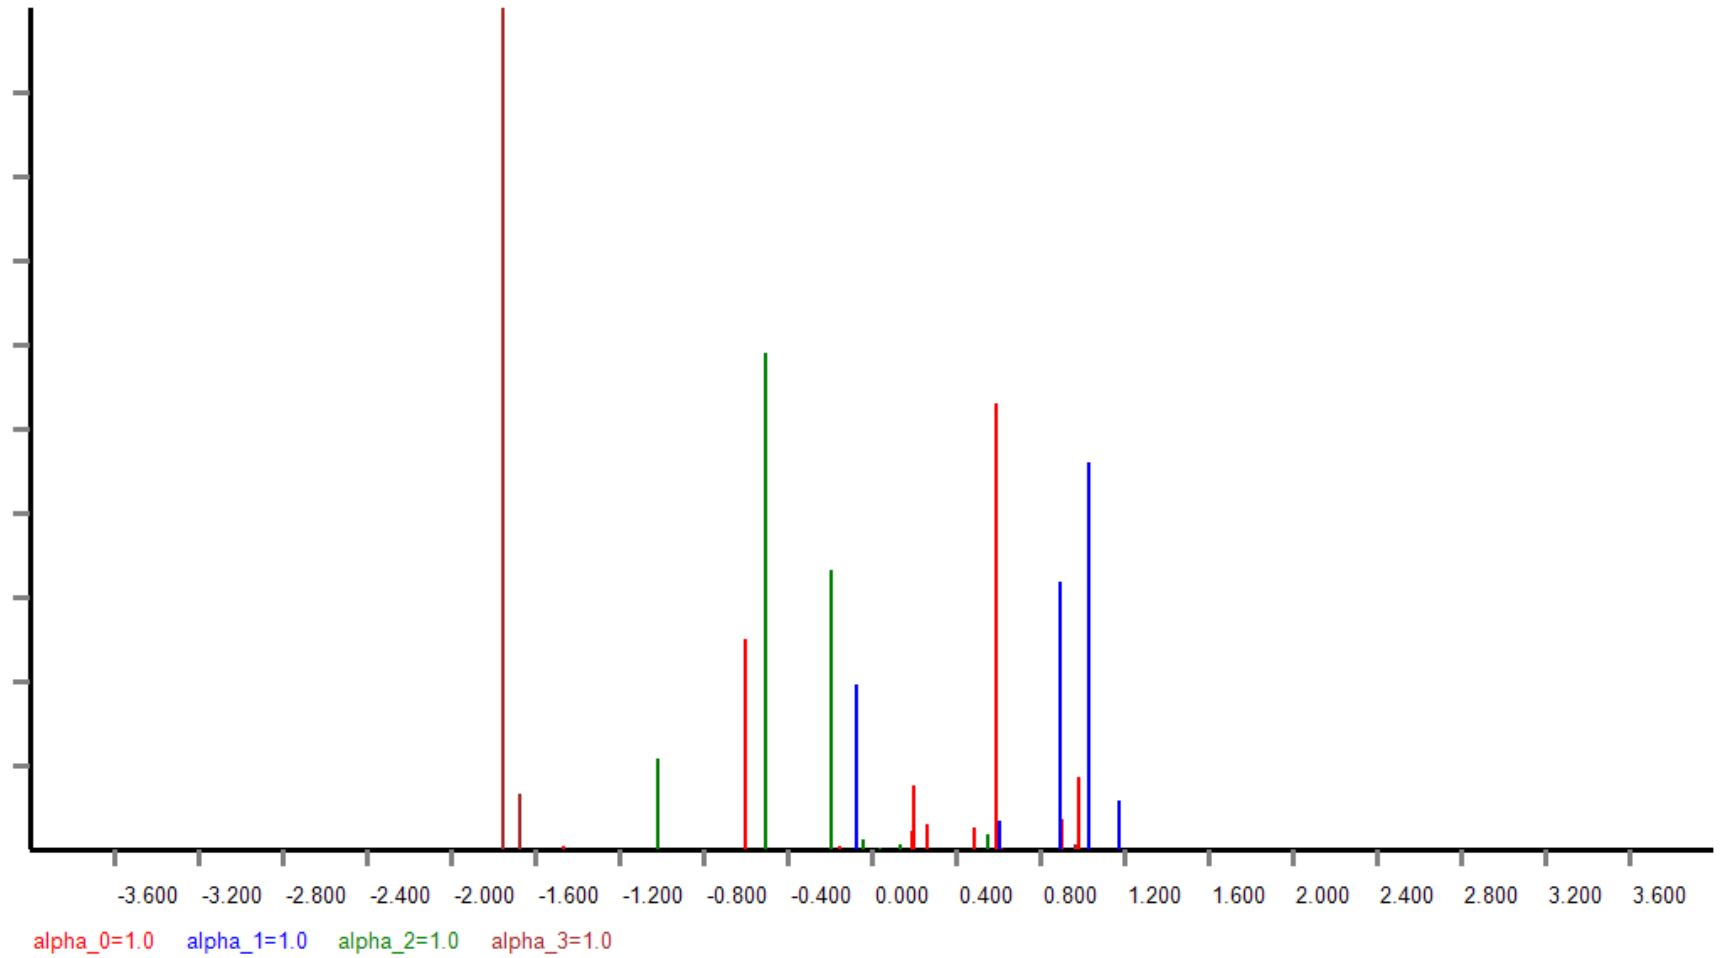
\includegraphics[width = 0.4\textwidth]{DPSample_1}
\end{subfloat}
\begin{subfloat}
\centering
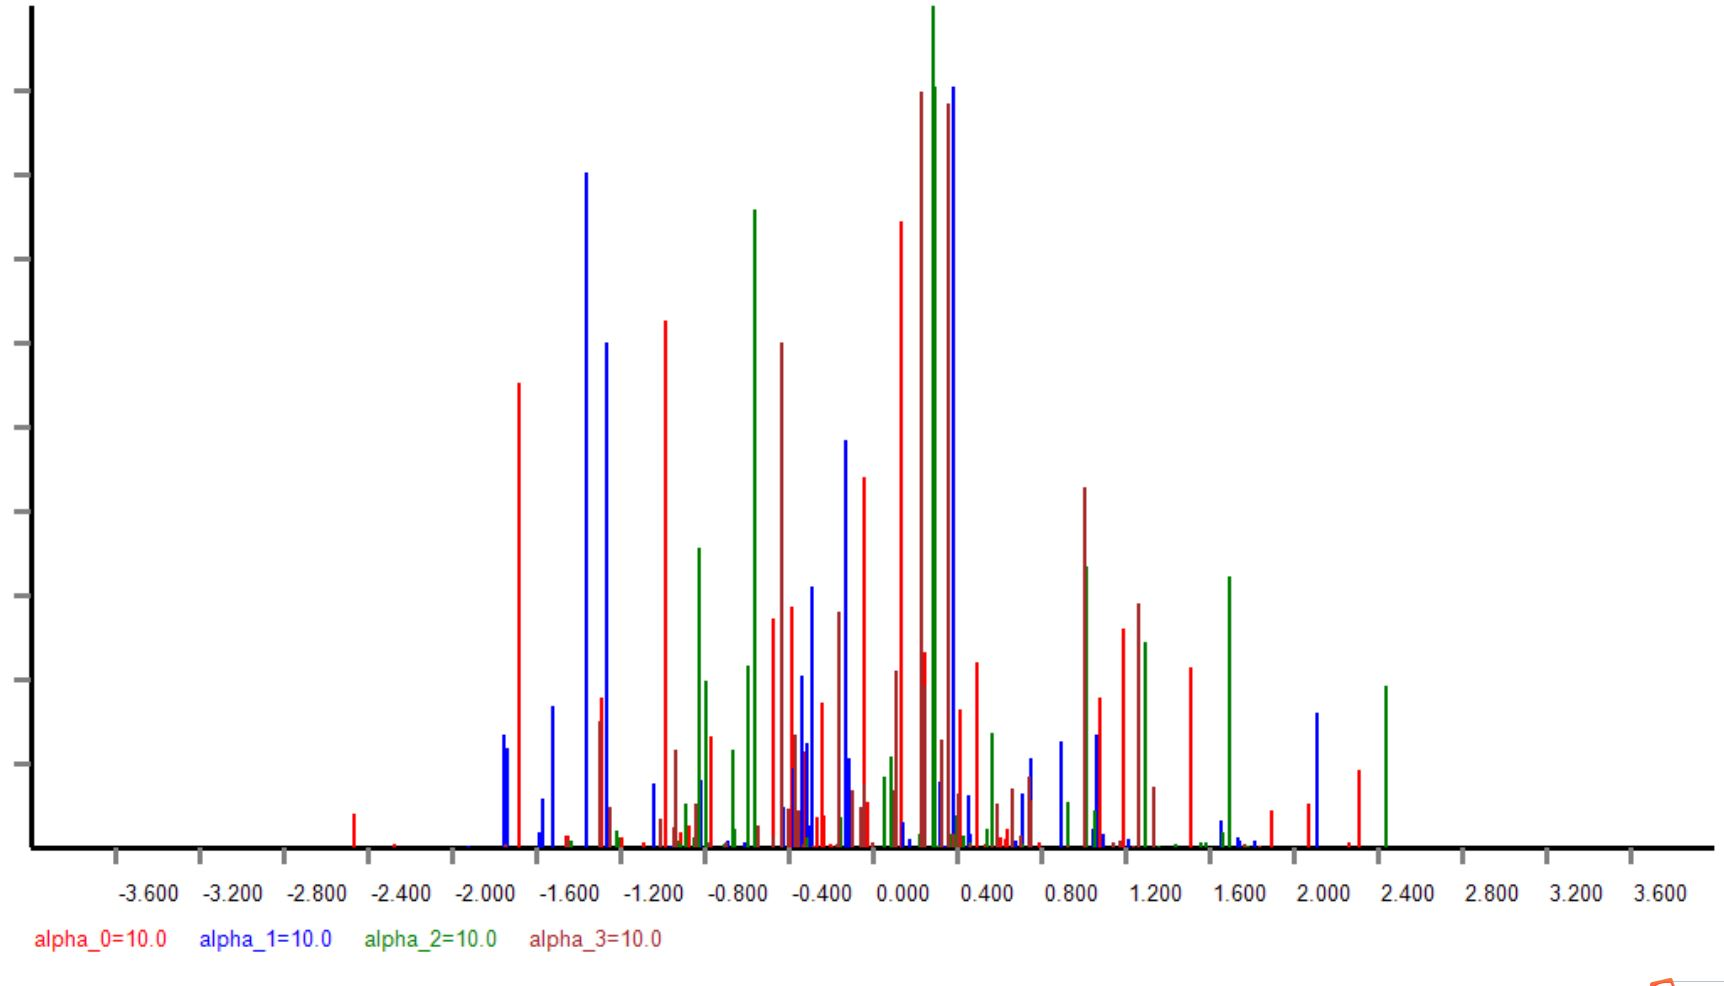
\includegraphics[width = 0.4\textwidth]{DPSample_10}
\end{subfloat}
\begin{subfloat}
\centering
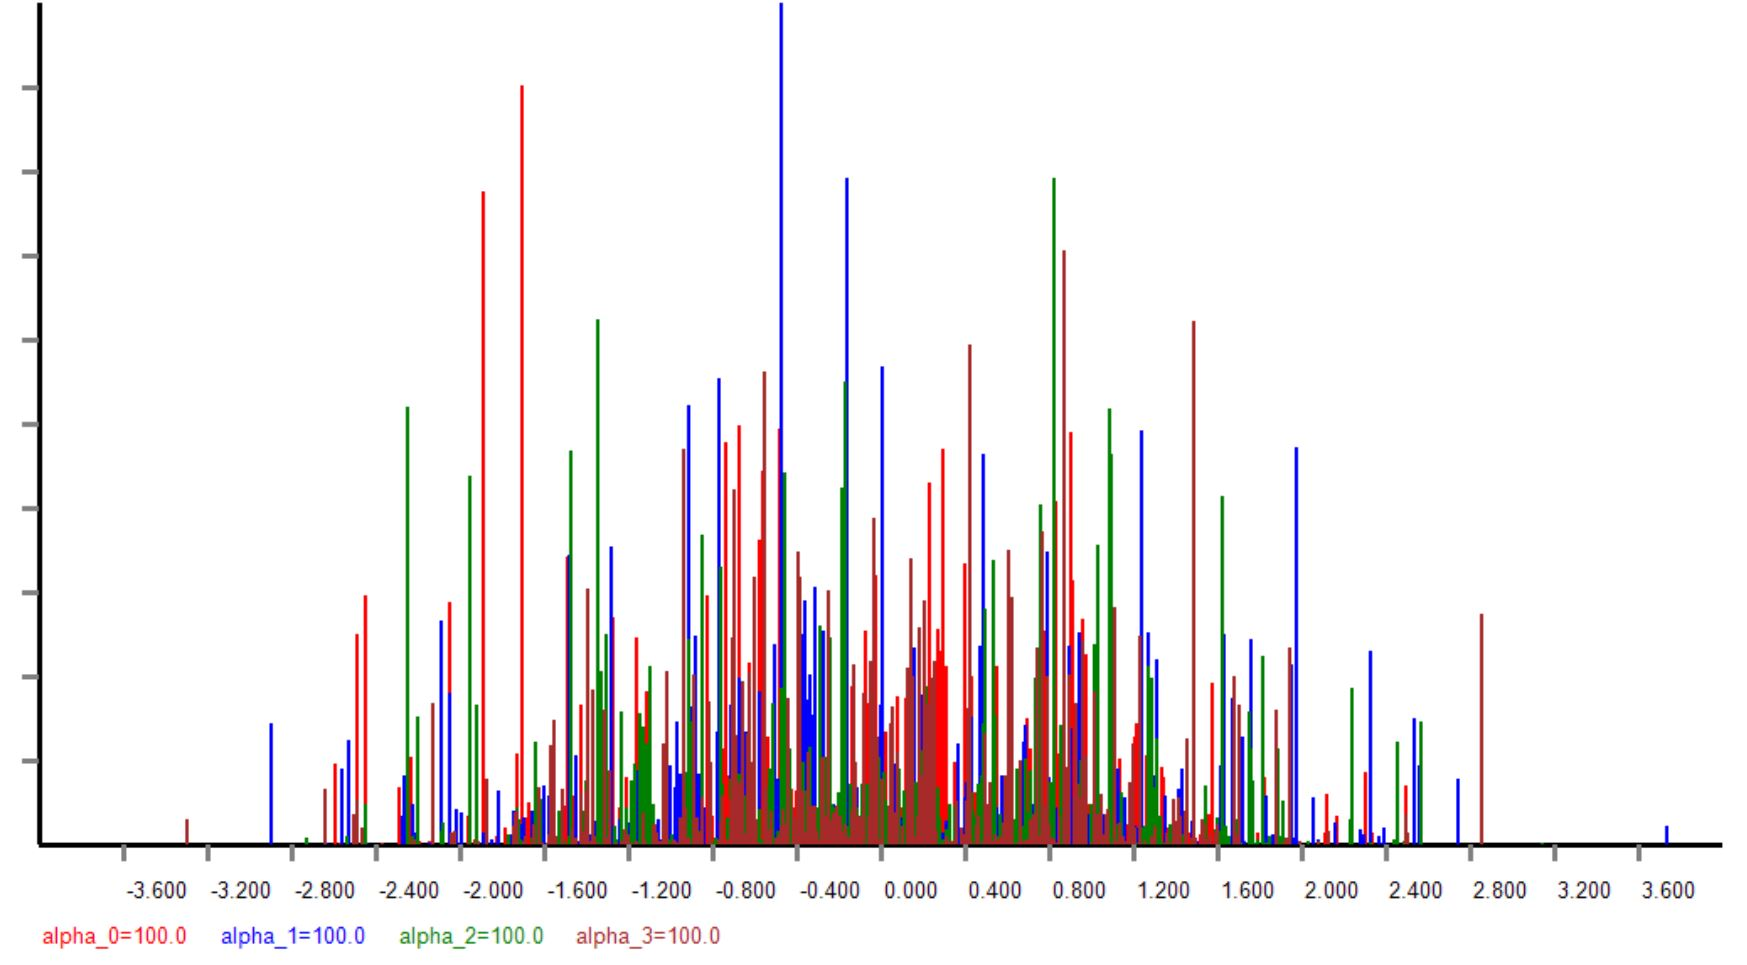
\includegraphics[width = 0.4\textwidth]{DPSample_100}
\end{subfloat}
\begin{subfloat}
\centering
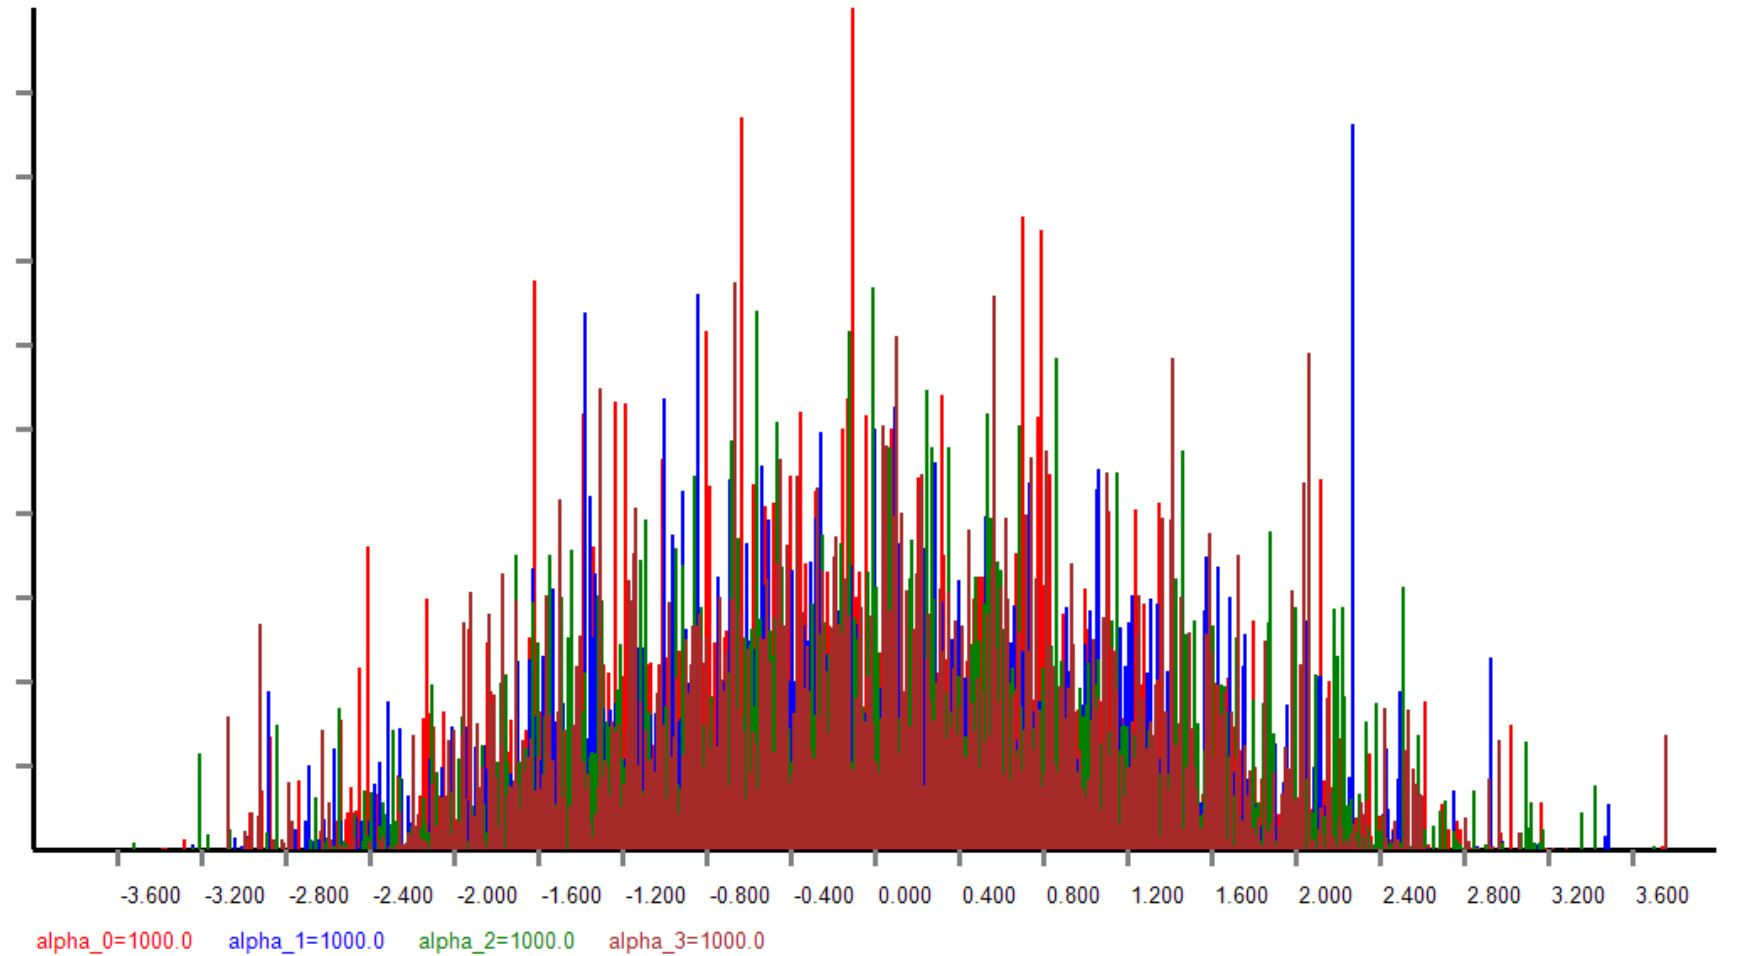
\includegraphics[width = 0.4\textwidth]{DPSample_1000}
\end{subfloat}
\caption{从DP中进行采样}
\end{figure}



\subsection{基于狄利克雷过程的聚类}

基于狄利克雷过程的聚类是这样的一个生成过程,我们有一个以$G_0,\alpha$为参数的狄利克雷过程$G$,在时刻$i$,我们从狄利克雷过程$G$中采样一个实数值$\phi_i$,该$\phi_i$为某个分布$F$的参数,我们从分布$F(\phi_i)$生成样本$x_i$。就与狄利克雷过程的聚类形式化为:

\begin{displaymath}
\begin{split}
G|G_0,\alpha &\sim G_0\\
\phi_i &\sim G\\
x_i|\phi_i &\sim F(\phi_i)\\
\end{split}
\end{displaymath}


\textbf{Polya Urn Scheme}
我们首先使用Polya Urn Scheme的方法来做狄利克雷过程的采样,并使用Gibbs Sampling的方法来训练基于狄利克雷过程聚类的训练。不失一般性的,我们假设$\phi_i$为最后一个球的颜色,则根据我们前边得到的:
\begin{displaymath}
\begin{split}
\phi_n | \phi_{1:n-1} \sim \frac{\alpha G_0(\phi_n)}{\alpha+n-1} + \frac{\sum_{j=1}^{n-1} \delta(\phi_n-\phi_j) }{\alpha+n-1}
\end{split}
\end{displaymath}
则给定$\phi_{1:n-1},x_i$,$\phi_n$的后验为:
\begin{displaymath}
\begin{split}
p(\phi_n | \phi_{1:n-1}, x_n) &\propto p_{new}(\phi_n, x_n) + p_{old}(\phi_n, x_n|\phi_{1:n-1})\\
p_{new}(\phi_n, x_n) &= \frac{\alpha G_0(\phi_n)F(x_n|\phi_n)}{\alpha + n-1}\\
p_{old}(\phi_n, x_n|\phi_{1:n-1}) &= \frac{ \sum_{j=1}^{n-1}F(x_n|\phi_n) \delta(\phi_j - \phi_n)}{\alpha + n-1} \\
p(\phi_n | \phi_{1:n-1}, x_n) &= \frac{\alpha G_0(\phi_n)F(x_n|\phi_n) + \sum_{j=1}^{n-1}F(x_n|\phi_n) \delta(\phi_n - \phi_j)} {
\int_{\phi}
\alpha G_0(\phi)F(x_n|\phi) + \sum_{j=1}^{n-1}F(x_n|\phi) \delta(\phi - \phi_j)
\mathrm{d} \phi
}\\
&= \frac{\alpha G_0(\phi_n)F(x_n|\phi_n) + \sum_{j=1}^{n-1}F(x_n|\phi_n) \delta(\phi_n - \phi_j)} {
\alpha \int_{\phi} G_0(\phi)F(x_n|\phi) \mathrm{d} \phi + \sum_{j=1}^{n-1}F(x_n|\phi_j)
}
\end{split}
\end{displaymath}

具体训练算法为:

\begin{minipage}{0.8\textwidth}\centering
\begin{algorithm}[H]
\textbf{DPMM Training with Polya Urn Scheme}($x_{i=1}^{n}, \alpha$):\\
\For{i=1,...,n}{
$\phi_i^0 =x_i$;
}
\For{t=0,1,...}{
\For{i=1,...,n}{
根据第$i$个样本$x_i$和上一轮训练的$\phi^{t-1}$采样一个新的$\phi _i^{t}$:
  $\phi_i^{t} \sim \frac{\alpha G_0(\phi_i^{t})F(x_i|\phi_i^{t}) + \sum_{j=1}^{n-1}F(x_i|\phi_j^{t-1}) \delta(\phi_i^t - \phi_j)} {
\alpha \int_{\phi} G_0(\phi)F(x_i|\phi) \mathrm{d} \phi + \sum_{j=1}^{n-1}F(x_i|\phi_j^{t-1})
}$\\
}
}

\end{algorithm}
\end{minipage}



具体的,假设分布$F$为一个均值为$\mu$方差为单位方差的正太分布,基础分布$G_0$为标准正太分布,则模型为:
\begin{displaymath}
\begin{split}
G_0 &= N(0,1)\\
G|G_0,\alpha &\sim DP(\alpha G_0(\mu))\\
\mu_i &\sim G(\mu)\\
x_i|\mu_i &\sim N(\mu_i, 1)\\
\end{split}
\end{displaymath}
则:
\begin{displaymath}
\begin{split}
G_0(\mu) &= \frac{1}{\sqrt{2\pi}} \exp{-\frac{\mu^2}{2}}\\
F(x|\mu) & = \frac{1}{\sqrt{2\pi}} \exp{-\frac{(x-\mu)^2}{2}}\\
G_0(\mu)F(x|\mu) &=  \frac{1}{2\pi} \exp{-\frac{(x-\mu)^2 + \mu^2}{2}}\\
\int_{\mu} G_0(\mu)F(x|\mu) \mathrm{d} \mu &= \int_{\mu}  \frac{1}{2\pi} \exp{-\frac{(x-\mu)^2 + \mu^2}{2}} \mathrm{d} \mu \\
&=  \int_{\mu} \frac{1}{2\pi} \exp{-(\mu^2-x\mu + \frac{x^2}{2})}  \mathrm{d} \mu \\
&=  \int_{\mu} \frac{1}{2\pi} \exp{-((\mu-\frac{x}{2})^2 + \frac{x^2}{4})}  \mathrm{d} \mu \\
&= \frac{1}{2\sqrt{\pi}} \exp{-\frac{x^2}{4}} 
 \int_{\mu} \frac{1}{\sqrt{\pi}} \exp{-(\mu-\frac{x}{2})^2}  \mathrm{d} \mu \\
&= \frac{1}{2\sqrt{\pi}} \exp{-\frac{x^2}{4}} \\
\end{split}
\end{displaymath}

\begin{displaymath}
\begin{split}
p(\mu_i^t | \mu_{-i}^{t-1}, x_i) &=\frac{\alpha G_0(\mu_i^{t})F(x_i|\mu_i^{t}) + \sum_{j \neq i}F(x_i|\mu_j^{t-1}) \delta(\mu_i^t - \mu_j)} {
\alpha \int_{\mu} G_0(\mu)F(x_i|\mu) \mathrm{d} \mu + \sum_{j \neq i}F(x_i|\mu_j^{t-1})
}\\
&= 
\end{split}
\end{displaymath}

\textbf{Stick Breaking Process}:使用polya urn scheme 来做Gibbs采样训练时,每次只能基于一个样本更新一个参数,这样子训练的时间复杂度会比较高。我们是不是可以安装聚好类的类别来更新参数呢?我们可以基于已有的模型采样每个样本从属的类$z_i$,然后基于采样得到的类别分配学习每个类的权重$\pi_k$,再根据采样得到的权重和类别重新采样类别的参数$\theta_k$。

我们先从FMM开始,FMM的定义如下:
\begin{displaymath}
\begin{split}
(x_i|z_i=k, \theta_k) \sim & F(x_i|\theta_k)\\
p(z_i=k) = & \pi_k\\
(\boldsymbol{\pi}|\alpha) \sim &Dir(\frac{\alpha}{K} . \mathrm{1}_{K} )\\
\theta_k \sim & H(\lambda)
\end{split}
\end{displaymath}
对于类别的指示变量$z_i$,我们有它的后验分布如下:
\begin{displaymath}
\begin{split}
&p(z_i=k | \mathbf{z}_{-i}, \mathbf{x}, \pi, \{\theta_k\}_{k=1}^{K}, \alpha, \lambda)\\
&= p(z_i=k | x_i, \pi, {\theta_k}_{k=1}^{K})\\
& \propto p(z_i=k | \pi, {\theta_k}_{k=1}^{K}) p(x_i| z_i=k, \pi, {\theta_k}_{k=1}^{K})\\
&= p(z_i=k | \pi) p(x_i| \theta_k)\\
&= \pi_k F(x_i|\theta_k)
\end{split}
\end{displaymath}
对于每个类的权重$\pi_k$,其后验分布如下:
\begin{displaymath}
\begin{split}
&p(\pi | \mathbf{z}, \mathbf{x}, \{\theta_k\}_{k=1}^{K}, \alpha, \lambda)\\
&= p(\pi | \mathbf{z}, \alpha)\\
&= Dir(n_1+\alpha/K, ... , n_K + \alpha/K)
\end{split}
\end{displaymath}
对每个类别的参数$\theta_k$,其后验分布如下:
\begin{displaymath}
\begin{split}
&p(\theta_k | \mathbf{\theta}_{-k}, \mathbf{z}, \mathbf{x}, \pi, \alpha, \lambda)\\
&= p(\theta_k | \mathbf{\theta}_{-k}, \mathbf{z}, \mathbf{x},\lambda)\\
&= p(\theta_k |\mathbf{z}, \mathbf{x},\lambda)\\
&\propto p(\theta_k |\lambda) p(\mathbf{x}_k|\theta_k)\\
\end{split}
\end{displaymath}

具体训练算法为:

\begin{minipage}{0.8\textwidth}\centering
\begin{algorithm}[H]
\textbf{FMM Training with Stick Breaking}($x_{i=1}^{n}, \alpha$):\\
\For{k=1,..., K}{
	随机初始化得到$\theta_k^{(0)}$;\\
}
\For{t=1,...}{
  \For{i=1,...,n}{
  	随机采样$z_i^{(t)}$:$p(z_i^{(t)}=k) \propto \pi_k F(x_i|\theta_k^{(t-1)})$;\\
  }
  $n_{k}^{(t)} = \sum_{i=1}^{n} \delta(z_i^{(t)}-k)$\\
  随机采样得到$\pi^{(t)}$: $\pi^{(t)} \sim Dir(n_1^{(t)} + \alpha/K, ..., n_K^{(t)} + \alpha/K)$;\\
  \For{k=1,..., K}{
  	随机采样得到$\theta_k^{(t)}$:$\theta_k^{(t)} \propto p(\theta_k |\lambda) p(\mathbf{x}_k|\theta_k^{(t-1)})$
  }
}
\end{algorithm}
\end{minipage}

该算法中类别的权重$\pi$是从Dirichlet分布中采样的。当$K \to \infty$的时候,采样这么一个类别的权重变为不可能。所以为了设计DPMM的训练,我们需要将$\pi$积掉。从而对于类别的指示变量$z_i$,我们有它的后验分布如下:
\begin{displaymath}
\begin{split}
&p(z_i=k | \mathbf{z}_{-i}, \mathbf{x}, \{\theta_k\}_{k=1}^{K}, \alpha, \lambda)\\
&= p(z_i=k |\mathbf{z}_{-i}, x_i, \theta_k, \alpha)\\
& \propto p(z_i=k|  \mathbf{z}_{-i}, \theta_k, \alpha)p(x_i|z_i=k, \mathbf{z}_{-i}, \theta_k, \alpha)\\
&= p(z_i=k | \mathbf{z}_{-i}, \alpha)p(x_i|\theta_k)\\
&=\frac{n_{k, -i}+\alpha / K}{n+\alpha -1} F(x_i|\theta_k)
\end{split}
\end{displaymath}

则,新的FMM的Gibbs Sampling训练算法为:

\begin{minipage}{0.8\textwidth}\centering
\begin{algorithm}[H]
\textbf{FMM Training with Stick Breaking}($x_{i=1}^{n}, \alpha$):\\
\For{k=1,..., K}{
随机初始化得到$\theta_k^{(0)}$;\\
}
\For{t=1,...}{
\For{i=1,...,n}{
随机采样$z_i^{(t)}$:$p(z_i^{(t)}=k) \propto \frac{n_{k, -i}+\alpha / K}{n+\alpha -1}F(x_i|\theta_k^{(t-1)})$, 其中 $n_{k, -i} = \sum_{j \neq i} \delta(z_j-k)$;\\
}

\For{k=1,..., K}{
随机采样得到$\theta_k^{(t)}$:$\theta_k^{(t)} \propto p(\theta_k |\lambda) p(\mathbf{x}_k|\theta_k^{(t-1)})$\\
}
}
\end{algorithm}
\end{minipage}
 
当我们使用DPMM来做聚类是,同FMM的区别是Gibbs Sampling对$z_i$的采样,当$z_i=k<K$时,$K$为当前的类别数:
\begin{displaymath}
\begin{split}
p(z_i=k | \mathbf{z}_{-i}, \mathbf{x}, \{\theta_k\}_{k=1}^{K}, \alpha, \lambda) = \frac{n_{k, -i}}{n+\alpha -1} F(x_i|\theta_{k}^{t-1})\\
\end{split}
\end{displaymath}
当$z_i$为一个新的类别,我们假设为$K+1$,则概率为:
\begin{displaymath}
\begin{split}
&p(z_i=K+1 | \mathbf{z}_{-i}, \mathbf{x}, \{\theta_k\}_{k=1}^{K}, \alpha, \lambda)\\
=&p(z_i=K+1 | \mathbf{z}_{-i}, x_i, \{\theta_k\}_{k=1}^{K}, \alpha, \lambda)\\
=&p(z_i=K+1 | \mathbf{z}_{-i}, \{\theta_k\}_{k=1}^{K}, \alpha, \lambda) p(x_i | z_i=K+1, \mathbf{z}_{-i}, \alpha, \lambda)\\
=&p(z_i=K+1 | \mathbf{z}_{-i}, \{\theta_k\}_{k=1}^{K}, \alpha, \lambda) p(x_i|\lambda)\\
=&\frac{\alpha}{n+\alpha-1} \int F(x_i|\theta)H(\theta|\lambda) \mathrm{d} \theta\\
\end{split}
\end{displaymath}

如果$H$和$F$共轭,我们便可以将$\theta$积掉,从而可以直接采样$z$。具体的DPMM的训练算法为:

\begin{minipage}{0.8\textwidth}\centering
\begin{algorithm}[H]
\textbf{DPMM Training with Stick Breaking}($x_{i=1}^{n}$):\\
$\alpha^{0} =1, K=n$;\\
\For{k=1,..., n}{
初始化$z_n = n$;\\
}
\For{t=1,...}{
\For{i=1,...,n}{
从类$z_i$中将$x_i$移除,如果类$z_i$为空,则删掉该类连同对应参数,$K--$;\\
随机采样$z_i^{(t)}$:\\
$p(z_i^{(t)}=k, k<K) \propto \frac{n_{k, -i}}{n+\alpha -1}F(x_i|\theta_k^{(t-1)})$, 其中 $n_{k, -i} = \sum_{j \neq i} \delta(z_j-k)$;\\
$p(z_i^{(t)}=K+1) \propto \frac{\alpha}{n+\alpha -1}\int F(x_i|\theta)H(\theta|\lambda) \mathrm{d} \theta$;\\
如果$z_i = K+1$, 采样一个新的$\theta_{K+1}$:\\
$p(\theta|x_i) = \frac{H(\theta)F(x_i|\theta)}{\int H(\theta)F(x_i|\theta) \mathrm{d} \theta}$;\\
}

\For{k=1,..., K}{
随机采样得到$\theta_k^{(t)}$:$\theta_k^{(t)} \propto p(\theta_k |\lambda) p(\mathbf{x}_k|\theta_k^{(t-1)})$\\
}

重新采样一个 $\alpha^{t} \sim p(\alpha|K, n, a, b)$ \footnote{Beyesian Density Estimation and Inference Using Mixtures}。
}
\end{algorithm}
\end{minipage}

% !Mode:: "TeX:UTF-8"

\chapter{BFGS}

问题: 求函数$f(x)$的最小值,即:
\begin{displaymath}
x^*=argmin(f(x))
\end{displaymath} 

\section{牛顿法}
假设我们可以构造一个序列$f(x_0), f(x_1), f(x_2), ..., f(x_n), ...$,使得$f(x_i)>f(x_{i+1}$,并且当$i \rightarrow \infty$时,$f(x_i) \rightarrow min(f(x))$.

假设$f(x)$是二次可导的,则可以用该函数在$x$处的二阶泰勒展开作为该函数的近似:
\begin{displaymath}
f(x+\Delta x) \approx \frac{f(x)}{0!} + \frac{\Delta x^T\bigtriangledown f(x)}{1!}+ \frac{\Delta x^T\bigtriangledown^2f(x)\Delta x}{2!} 
\end{displaymath}
其中, $\bigtriangledown f(x)$和$\bigtriangledown^2f(x)$分别是$f(x)$在点$x$处的梯度和Hessian矩阵。我们令$x_{n+1}=x_n+\Delta x$,并将上公式改写为:
\begin{displaymath}
h_n(\Delta x)=f(x_n)+\Delta x^T\mathbf{g}_n +\frac{1}{2}\Delta x^T \mathbf{H}_n\Delta x
\end{displaymath}
其中, $\mathbf{g}_n$和$\mathbf{H}_n$分别是$f(x)$在点$x_n$处的梯度和Hessian矩阵。

为得到原始函数$f(x)$的最小值,我们现在有其在点$x_n$处的近似,我们可以将点$x_n$移动到点$x_n + \Delta x$处获得一个更小值,那么如何选择$\Delta x$。基于近似函数$h_n(\Delta x)$,我们选择使得该近似函数最小的$\Delta x$,由于该近似函数为凸函数(假设$\mathbf{H}_n$为正定矩阵),全局最小值处导数为0,故而:
\begin{displaymath}
\frac{\partial h_n(\Delta x)}{\partial \Delta x} = \mathbf{g}_n + \mathbf{H}_n \Delta x = 0
\end{displaymath}
从而得到一个比较好的基于当前点$x_n$的移动方向$\Delta x$:
\begin{displaymath}
\Delta x = -\mathbf{H}_n^{-1}\mathbf{g}_n
\end{displaymath}

从而我们有牛顿优化算法如下:

\begin{minipage}{0.8\textwidth}\centering
\begin{algorithm}[H]
\textbf{NewtonRaphson}($f$,$x_0$):\\
\For{n=0,1,...(until converged)}{
Compute $\mathbf{g}_n$ and $\mathbf{H}_n^{-1}$ for $x_n$\\
$d=\mathbf{H}_n^{-1}\mathbf{g}_n$\\
$x_{n+1} \leftarrow x_n - d$\\
}
\end{algorithm}
\end{minipage}

\section{阻尼牛顿法}

由于函数$h_n(\Delta x)$仅仅为原始函数的近似,故而该函数的最低点并不一定是原始函数的最低点,如果一次更新到该近似函数的极值点可能会导致$f(x_{n+1}) > f(x_n)$的情况发生。一个比较合理的选择是向方向$d$移动一段距离,即引入步长$\alpha$。步长$\alpha$的计算可以任意的线性搜索算法来得到。

\begin{minipage}{0.8\textwidth}\centering
\begin{algorithm}[H]
\textbf{NewtonRaphson}($f$,$x_0$):\\
\For{n=0,1,...(until converged)}{
Compute $\mathbf{g}_n$ and $\mathbf{H}_n^{-1}$ for $x_n$\\
$d=\mathbf{H}_n^{-1}\mathbf{g}_n$\\
$\alpha = \min \limits_{\alpha \geqq 0} f(x_n-\alpha d)$\\
$x_{n+1} \leftarrow x_n - \alpha d$\\
}
\end{algorithm}
\end{minipage}
 
牛顿法和阻尼牛顿法都需要对Hessian矩阵$\mathbf{H}$进行计算(函数参数为$N$,计算量为$N^2$)。当函数参数比较多时,每次更新的计算量比较大。如何计算一个近似的矩阵来替代Hessian矩阵成为加速牛顿法的主要思路,该一系列方法成为拟牛顿法。

\section{拟牛顿法}
拟牛顿法的基本思想是使用一个近似矩阵来模拟Hessian矩阵。那么什么样的矩阵才适合作为Hessian矩阵的近似呢?基于前面近似函数:
\begin{displaymath}
h_n(\Delta x)=f(x_n)+\Delta x^T\mathbf{g}_n +\frac{1}{2}\Delta x^T \mathbf{H}_n\Delta x
\end{displaymath}
一个好的近似函数应该满足在点$x_{n+1}$和$x_n$处的一阶导数同原始函数一致,即:
\begin{displaymath}
\begin{split}
\Delta h_n(x_n) &= \mathbf{g}_n\\
\Delta h_n(x_{n+1}) &= \mathbf{g}_{n+1}
\end{split}
\end{displaymath}
从而有:
\begin{displaymath}
\Delta h_n(x_{n+1}) -\Delta h_n(x_n) = \mathbf{g}_{n+1} - \mathbf{g}_n
\end{displaymath}
根据中值定理在点$x_n$和$x_{n+1}$之间存在某点$x_n^{'}$该处的Hessian矩阵$B_{n+1}$满足:
\begin{displaymath}
B_{n+1}(x_{n+1} - x_n) = \Delta h_n(x_{n+1}) -\Delta h_n(x_{n})  = \mathbf{g}_{n+1} - \mathbf{g}_n
\end{displaymath}

% \begin{figure}[htbp]
% \centering
% 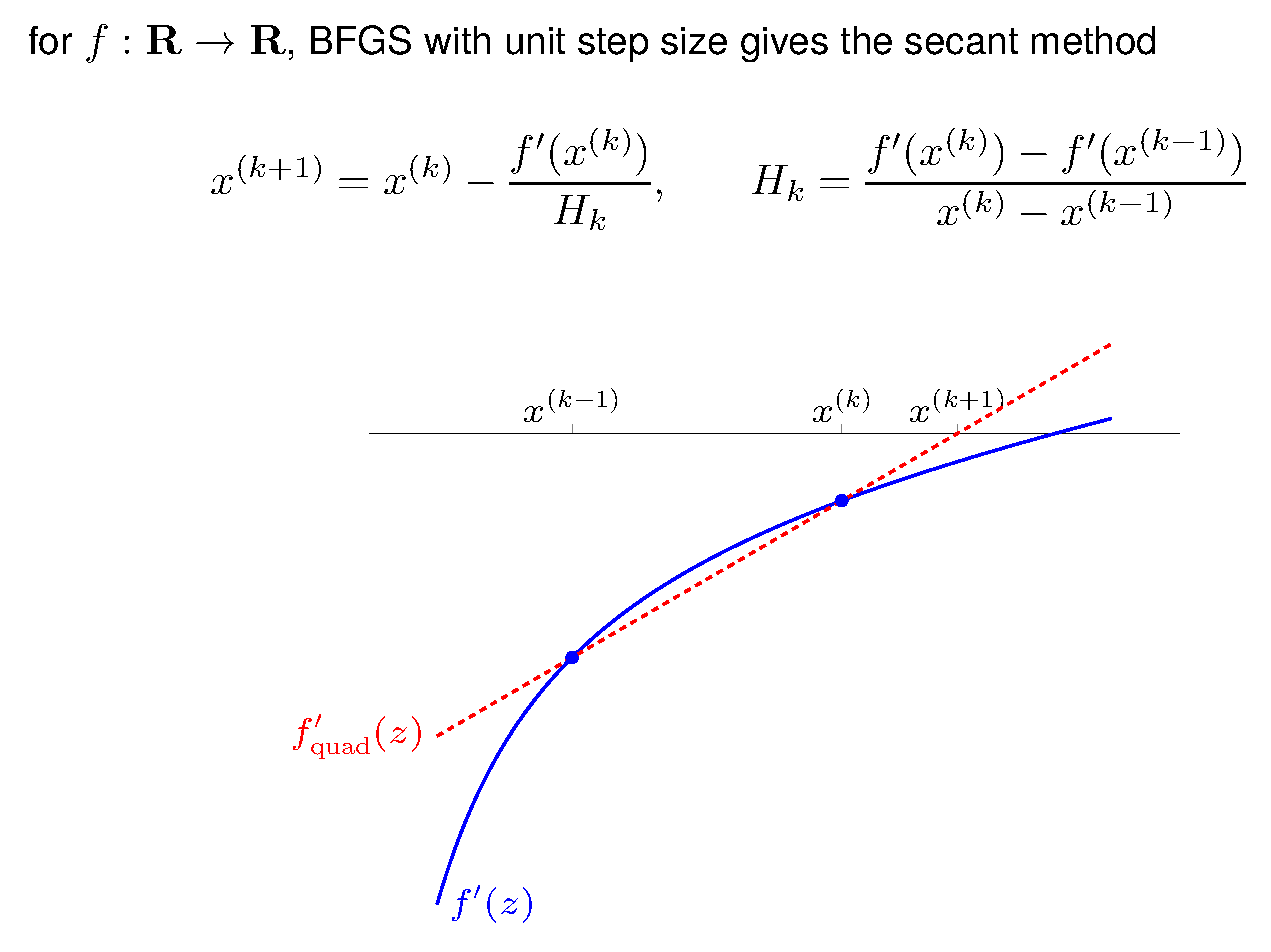
\includegraphics[width = 0.8\textwidth]{SecantCondition}
% \end{figure}

我们令$\mathbf{s}_n=x_{n+1}-x_{n}$,$\mathbf{y}_n=\mathbf{g}_{n+1} - \mathbf{g}_n$,$D_n = B_n^{-1}$则有:
\begin{displaymath}
\begin{split}
B_{n+1}\mathbf{s}_n = \mathbf{y}_n\\
\mathbf{s}_n = D_{n+1} \mathbf{y}_n
\end{split}
\end{displaymath}
该约束条件称为Secant条件。Secant条件可以保证选取的近似Hessian矩阵使得近似函数在点$x_{n-1}$和$x_n$处的一阶导数同原始函数一致。


\section{DFP算法}
DFP算法是由Davidon, Fletcher, Powell三人提出的拟牛顿法。DFP算法的基本思路是从一个对称矩阵$D_0$开始,采用迭代的方式$D_{n+1}=D_n+\Delta D_n, n=0,1,2,...$来获得一个Hessian逆矩阵的近似矩阵。那么如何计算$\Delta D_n$。我们知道如果$D_n$是对称矩阵,那么只要$\Delta D_n$为对称矩阵,则得到的$D_{n+1}$也为对称矩阵。不失一般性的,我们假设$\Delta D_n$的形式为$\Delta D_n = \alpha\mathbf{uu}^T + \beta \mathbf{vv}^T$,其中$\alpha$和$\beta$为待定参数,$\mathbf{u}$和$\mathbf{v}$为待定向量。

根据Secant条件我们有:
\begin{displaymath}
\begin{split}
\mathbf{s}_n &= D_{n+1} \mathbf{y}_n\\
 &= (D_n + \Delta D) \mathbf{y}_n\\
 &= (D_n + \alpha\mathbf{uu}^T + \beta \mathbf{vv}^T) \mathbf{y}_n\\
 &= (D_n + \alpha\mathbf{uu}^T + \beta \mathbf{vv}^T) \mathbf{y}_n\\
\mathbf{s}_n &= D_n \mathbf{y}_n + \alpha\mathbf{uu}^T \mathbf{y}_n + \beta \mathbf{vv}^T \mathbf{y}_n\\
&= D_n \mathbf{y}_n + (\alpha\mathbf{u}^T \mathbf{y}_n)\mathbf{u} + (\beta \mathbf{v}^T \mathbf{y}_n)\mathbf{v}
\end{split}
\end{displaymath}
令$\alpha=\frac{1}{\mathbf{u}^T \mathbf{y}_n}$,$\beta = \frac{-1}{\mathbf{v}^T \mathbf{y}_n}$,则有:
\begin{displaymath}
\begin{split}
\mathbf{s}_n = D_n \mathbf{y}_n + \mathbf{u} -  \mathbf{v}\\
\mathbf{u} -  \mathbf{v} =\mathbf{s}_n - D_n \mathbf{y}_n 
\end{split}
\end{displaymath}

为满足secant条件,我们令$\mathbf{u}= \mathbf{s}_n$, $\mathbf{v} = D_n\mathbf{y}_n$,从而:
\begin{displaymath}
\begin{split}
\alpha &=\frac{1}{\mathbf{u}^T \mathbf{y}_n} =\frac{1}{\mathbf{s}_n^T\mathbf{y}_n}\\
\beta &= \frac{-1}{\mathbf{v}^T \mathbf{y}_n} = \frac{-1}{(D_n\mathbf{y})^T \mathbf{y}_n} = \frac{-1}{\mathbf{y}^T D_n \mathbf{y}_n}\\
\end{split}
\end{displaymath}
故而有:
\begin{displaymath}
\Delta D_n = \alpha\mathbf{uu}^T + \beta \mathbf{vv}^T
=\frac{\mathbf{uu}^T}{\mathbf{s}_n^T\mathbf{y}_n} + \frac{-\mathbf{vv}^T}{\mathbf{y}_n^T D_n \mathbf{y}_n}
=\frac{\mathbf{s}_n\mathbf{s}_n^T}{\mathbf{s}_n^T\mathbf{y}_n} - \frac{D_n\mathbf{y}_n\mathbf{y}_n^TD_n}{\mathbf{y}_n^T D_n \mathbf{y}_n}
\end{displaymath}

DFP算法具体如下:

\begin{minipage}{0.8\textwidth}\centering
\begin{algorithm}[H]
\textbf{DFP}($f$,$\epsilon$, $x_0$):\\
$D_0 = I$\\
\For{n=0,1,...(until $\lVert \mathbf{g}_n \rVert \leq \epsilon$)}{
$d_n=D_n\mathbf{g}_n$\\
$\alpha = \min \limits_{\alpha \geqq 0} f(x_n- \alpha d_n)$\\
$\mathbf{s}_n = \alpha d_n$, $x_{n+1} = x_n + \mathbf{s}_n$, $\mathbf{y}_n = \mathbf{g}_{n+1}-\mathbf{g}_n$ \\
$D_{n+1}=D_n + \frac{\mathbf{s}_n\mathbf{s}_n^T}{\mathbf{s}_n^T\mathbf{y}_n} - \frac{D_n\mathbf{y}_n\mathbf{y}_n^TD_n}{\mathbf{y}^T D_n \mathbf{y}_n}$
}
\end{algorithm}
\end{minipage}

另一个证明的思路是:
\begin{displaymath}
\begin{split}
\min & _{D_{n+1}}{\lVert D_{n+1}-D_n \rVert ^2}\\
s.t.~~~~ &s_n = D_{n+1}\mathbf{y}_n\\
&D_{n+1}~~ is~ symmetric
\end{split}
\end{displaymath}
%  条件 $D_{n+1}~~ is ~ symmetric$能够改写为 $D_{n+1} = D_n + \Delta D_n$,其中$\Delta D_n =\mathbf{uu}^T + \mathbf{vv}^T$。则优化问题变为:
% \begin{displaymath}
% \begin{split}
% \min & \limits_{\mathbf{u,v}}{\lVert \mathbf{uu}^T + \mathbf{vv}^T \rVert ^2}\\
% s.t.~~~~ &s_n = (D_n + \mathbf{uu}^T + \mathbf{vv}^T)\mathbf{y}_n\\
% &D_0=I
% \end{split}
% \end{displaymath}
% 证不下去了.....

\section{BFGS算法}

BFGS算法是由Broden, Fletcher, Goldfarb, Shanno四人提出的。同DFP算法类似,BFGS算法同样从一个对称矩阵$B_0$开始,采用迭代的方式生成近似矩阵$B_{n+1}=B_n+\Delta B_n, n=0,1,2,...$。需要指出的是DFP方法获取的是Hessian逆矩阵的近似矩阵,而BFGS方法则是获取Hessian矩阵的近似矩阵。同DFP的证明一样,我们另$\Delta B_n = \alpha \mathbf{uu}^T + \beta \mathbf{vv}^T$,其中$\alpha$和$\beta$为待定参数,$\mathbf{u}$和$\mathbf{v}$为待定向量。
\begin{figure}[htbp]
\centering
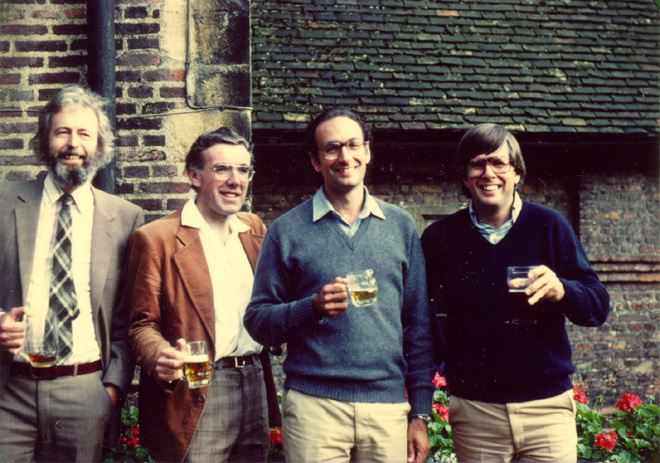
\includegraphics[width = 0.8\textwidth]{Broyden-Fletcher-Goldfarb-Shanno}
\end{figure}

根据Secant条件我们有:
\begin{displaymath}
\begin{split}
\mathbf{y}_n &= B_{n+1} \mathbf{s}_n\\
 &= (B_n + \Delta B) \mathbf{s}_n\\
 &= (B_n + \alpha\mathbf{uu}^T + \beta \mathbf{vv}^T) \mathbf{s}_n\\
 &= (B_n + \alpha\mathbf{uu}^T + \beta \mathbf{vv}^T) \mathbf{s}_n\\
\mathbf{y}_n &= B_n \mathbf{s}_n + \alpha\mathbf{uu}^T \mathbf{s}_n + \beta \mathbf{vv}^T \mathbf{s}_n\\
&= B_n \mathbf{s}_n + (\alpha\mathbf{u}^T \mathbf{s}_n)\mathbf{u} + (\beta \mathbf{v}^T \mathbf{s}_n)\mathbf{v}
\end{split}
\end{displaymath}
令$\alpha=\frac{1}{\mathbf{u}^T \mathbf{s}_n}$,$\beta = \frac{-1}{\mathbf{v}^T \mathbf{s}_n}$,则有:
\begin{displaymath}
\begin{split}
\mathbf{y}_n = B_n \mathbf{s}_n + \mathbf{u} -  \mathbf{v}\\
\mathbf{u} -  \mathbf{v} =\mathbf{y}_n - B_n \mathbf{s}_n 
\end{split}
\end{displaymath}

为满足secant条件,我们令$\mathbf{u}= \mathbf{y}_n$, $\mathbf{v} = B_n\mathbf{s}_n$,从而:
\begin{displaymath}
\begin{split}
\alpha &=\frac{1}{\mathbf{u}^T \mathbf{s}_n} =\frac{1}{\mathbf{y}_n^T\mathbf{s}_n}\\
\beta &= \frac{-1}{\mathbf{v}^T \mathbf{s}_n} = \frac{-1}{(B_n\mathbf{s}_n)^T \mathbf{s}_n} = \frac{-1}{\mathbf{s}_n^T B_n \mathbf{s}_n}\\
\end{split}
\end{displaymath}
故而有:
\begin{displaymath}
\Delta B_n = \alpha\mathbf{uu}^T + \beta \mathbf{vv}^T
=\frac{\mathbf{uu}^T}{\mathbf{y}_n^T\mathbf{s}_n} + \frac{-\mathbf{vv}^T}{\mathbf{s}_n^T B_n \mathbf{s}_n}
=\frac{\mathbf{y}_n\mathbf{y}_n^T}{\mathbf{y}_n^T\mathbf{s}_n} - \frac{B_n\mathbf{s}_n\mathbf{s}_n^TB_n}{\mathbf{s}^T B_n \mathbf{s}_n}
\end{displaymath}

BFGS算法具体如下:

\begin{minipage}{0.8\textwidth}\centering
\begin{algorithm}[H]
\textbf{BFGS}($f$,$\epsilon$, $x_0$):\\
$B_0 = I$\\
\For{n=0,1,...(until $\lVert \mathbf{g}_n \rVert \leq \epsilon$)}{
$d_n=B_n^{-1}\mathbf{g}_n$\\
$\alpha = \min \limits_{\alpha \geqq 0} f(x_n- \alpha d_n)$\\
$\mathbf{s}_n = \alpha d_n$, $x_{n+1} = x_n + \mathbf{s}_n$, $\mathbf{y}_n = \mathbf{g}_{n+1}-\mathbf{g}_n$ \\
$B_{n+1}=B_n + \frac{\mathbf{y}_n\mathbf{y}_n^T}{\mathbf{y}_n^T\mathbf{s}_n} - \frac{B_n\mathbf{s}_n\mathbf{s}_n^TB_n}{\mathbf{s}^T B_n \mathbf{s}_n}$
}
\end{algorithm}
\end{minipage}

另一个证明的思路是:
\begin{displaymath}
\begin{split}
\min & _{B_{n+1}}{\lVert B_{n+1}-B_n \rVert ^2}\\
s.t.~~~~ &y_n = B_{n+1}\mathbf{s}_n\\
&B_{n+1}~~ is~ symmetric
\end{split}
\end{displaymath}

我们看到,在BFGS算法当中我们需要计算矩阵$B_n$的逆,常用的方法是利用Sherman-Morrison公式来直接使用$B_n^{-1}$来直接计算$B_{n+1}^{-1}$:
\begin{displaymath}
\begin{split}
B_{n+1}^{-1} = \left( I- \frac{\mathbf{s}_n\mathbf{y}_n^T}{\mathbf{y}_n^T\mathbf{s}_n} \right) B_n^{-1} \left( I- \frac{\mathbf{y}_n\mathbf{s}_n^T}{\mathbf{y}_n^T\mathbf{s}_n} \right) +\frac{\mathbf{s}_n\mathbf{s}_n^T}{\mathbf{y}_n^T\mathbf{s}_n}
\end{split}
\end{displaymath}
我们令$B^{-1}=D$,则公式为
\begin{displaymath}
\begin{split}
D_{n+1} = \left( I- \frac{\mathbf{s}_n\mathbf{y}_n^T}{\mathbf{y}_n^T\mathbf{s}_n} \right) D_n \left( I- \frac{\mathbf{y}_n\mathbf{s}_n^T}{\mathbf{y}_n^T\mathbf{s}_n} \right) +\frac{\mathbf{s}_n\mathbf{s}_n^T}{\mathbf{y}_n^T\mathbf{s}_n}
\end{split}
\end{displaymath}

Sherman-Morison公式为:
\begin{displaymath}
(A+\frac{uv^T}{t})^{-1} = A^{-1} - \frac{A^{-1}uv^TA^{-1}}{t+v^TA^{-1}u} 
\end{displaymath}
证明过程如下:
\begin{displaymath}
\begin{split}
&(A+\frac{uv^T}{t})*( A^{-1} - \frac{A^{-1}uv^TA^{-1}}{t+v^TA^{-1}u})\\
=&AA^{-1} + \frac{uv^TA^{-1}}{t} - \frac{AA^{-1}uv^TA^{-1}}{t+v^TA^{-1}u}-\frac{uv^TA^{-1}uv^TA^{-1}}{t*(t+v^TA^{-1}u)}\\
=&I + \frac{uv^TA^{-1}}{t} -\frac{tuv^TA^{-1} + uv^TA^{-1}uv^TA^{-1}}{t*(t+v^TA^{-1}u)}\\
=& I + \frac{uv^TA^{-1}}{t} -\frac{u(t)v^TA^{-1} + u(v^TA^{-1}u)v^TA^{-1}}{t*(t+v^TA^{-1}u)}\\
=& I + \frac{uv^TA^{-1}}{t} -\frac{u(t+v^TA^{-1}u)v^TA^{-1}}{t*(t+v^TA^{-1}u)}\\
=& I + \frac{uv^TA^{-1}}{t} -\frac{uv^TA^{-1}}{t}\\
=& I
\end{split}
\end{displaymath}

我们忽略掉更新算法中的$n$,使用Sherman-Morison公式,我们有:
\begin{displaymath}
\begin{split}
&(B + \frac{\mathbf{y}\mathbf{y}^T}{\mathbf{y}^T\mathbf{s}} - \frac{B\mathbf{s}\mathbf{s}^TB}{\mathbf{s}^T B \mathbf{s}})^{-1}
=(B + \frac{\mathbf{y}\mathbf{y}^T}{\mathbf{y}^T\mathbf{s}})^{-1} -
\frac{(B + \frac{\mathbf{y}\mathbf{y}^T}{\mathbf{y}^T\mathbf{s}})^{-1}Bss^TB(B + \frac{\mathbf{y}\mathbf{y}^T}{\mathbf{y}^T\mathbf{s}})^{-1}}{-s^TBs+s^TB(B + \frac{\mathbf{y}\mathbf{y}^T}{\mathbf{y}^T\mathbf{s}})^{-1}Bs}\\
=&(B^{-1}-\frac{B^{-1}\mathbf{yy}^TB^{-1}}{\mathbf{y}^T\mathbf{s} + \mathbf{y}^TB^{-1}\mathbf{y}}) +
(B^{-1}-\frac{B^{-1}\mathbf{yy}^TB^{-1}}{\mathbf{y}^T\mathbf{s} + \mathbf{y}^TB^{-1}\mathbf{y}})
\frac{Bss^TB}{s^TBs-s^TB (B^{-1}-\frac{B^{-1}\mathbf{yy}^TB^{-1}}{\mathbf{y}^T\mathbf{s} + \mathbf{y}^TB^{-1}\mathbf{y}}) Bs}
(B^{-1}-\frac{B^{-1}\mathbf{yy}^TB^{-1}}{\mathbf{y}^T\mathbf{s} + \mathbf{y}^TB^{-1}\mathbf{y}})\\
=&(B^{-1}-\frac{B^{-1}\mathbf{yy}^TB^{-1}}{\mathbf{y}^T\mathbf{s} + \mathbf{y}^TB^{-1}\mathbf{y}}) +
(B^{-1}-\frac{B^{-1}\mathbf{yy}^TB^{-1}}{\mathbf{y}^T\mathbf{s} + \mathbf{y}^TB^{-1}\mathbf{y}})
\frac{Bss^TB}{
\frac{s^T\mathbf{yy}^Ts}{\mathbf{y}^T\mathbf{s} + \mathbf{y}^TB^{-1}\mathbf{y}}
}
(B^{-1}-\frac{B^{-1}\mathbf{yy}^TB^{-1}}{\mathbf{y}^T\mathbf{s} + \mathbf{y}^TB^{-1}\mathbf{y}})\\
=&B^{-1}-\frac{B^{-1}\mathbf{yy}^TB^{-1}}{\mathbf{y}^T\mathbf{s} + \mathbf{y}^TB^{-1}\mathbf{y}}
+\frac{ss^T\mathbf{y}^T\mathbf{s} + ss^T\mathbf{y}^TB^{-1}\mathbf{y}}{s^T\mathbf{yy}^Ts}
-\frac{s\mathbf{y}^TB^{-1}}{s^T\mathbf{y}}
-\frac{B^{-1}\mathbf{y}s^T}{s^T\mathbf{y}}
+\frac{B^{-1}\mathbf{y}\mathbf{y}^TB^{-1}}{\mathbf{y}^T\mathbf{s} + \mathbf{y}^TB^{-1}\mathbf{y}}\\
=&B^{-1}
+\frac{ss^T\mathbf{y}^T\mathbf{s} + ss^T\mathbf{y}^TB^{-1}\mathbf{y}}{s^T\mathbf{yy}^Ts}
-\frac{s\mathbf{y}^TB^{-1}}{s^T\mathbf{y}}
-\frac{B^{-1}\mathbf{y}s^T}{s^T\mathbf{y}}\\
=&B^{-1}
+\frac{ss^T}{s^T\mathbf{y}}
+\frac{ss^T\mathbf{y}^TB^{-1}\mathbf{y}}{s^T\mathbf{yy}^Ts}
-\frac{s\mathbf{y}^TB^{-1}}{s^T\mathbf{y}}
-\frac{B^{-1}\mathbf{y}s^T}{s^T\mathbf{y}}\\
=&B^{-1}
+\frac{ss^T}{s^T\mathbf{y}}
+\frac{s\mathbf{y}^TB^{-1}\mathbf{y}s^T}{s^T\mathbf{yy}^Ts}
-\frac{s\mathbf{y}^TB^{-1}}{s^T\mathbf{y}}
-\frac{B^{-1}\mathbf{y}s^T}{s^T\mathbf{y}} // \mathbf{y}^TB^{-1}\mathbf{y}~is~scalar \\
=&B^{-1}(I-\frac{\mathbf{y}s^T}{s^T\mathbf{y}})-\frac{s\mathbf{y}^TB^{-1}}{s^T\mathbf{y}}(I-\frac{\mathbf{y}s^T}{s^T\mathbf{y}}) + \frac{ss^T}{s^T\mathbf{y}}\\
=&(I-\frac{s\mathbf{y}^T}{s^T\mathbf{y}})B^{-1}(I-\frac{\mathbf{y}s^T}{s^T\mathbf{y}}) + \frac{ss^T}{s^T\mathbf{y}}\\
\end{split}
\end{displaymath}

证明过程中用到的一些辅助证明:
\begin{displaymath}
\begin{split}
&(B + \frac{\mathbf{y}\mathbf{y}^T}{\mathbf{y}^T\mathbf{s}})^{-1}
=B^{-1}-\frac{B^{-1}\mathbf{yy}^TB^{-1}}{\mathbf{y}^T\mathbf{s} + \mathbf{y}^TB^{-1}\mathbf{y}}\\
&s^TBs-s^TB (B^{-1}-\frac{B^{-1}\mathbf{yy}^TB^{-1}}{\mathbf{y}^T\mathbf{s} + \mathbf{y}^TB^{-1}\mathbf{y}}) Bs
=s^TBs-s^TBB^{-1}Bs+\frac{s^TBB^{-1}\mathbf{yy}^TB^{-1}Bs}{\mathbf{y}^T\mathbf{s} + \mathbf{y}^TB^{-1}\mathbf{y}}\\
=&s^TBs-s^TBs+\frac{s^T\mathbf{yy}^Ts}{\mathbf{y}^T\mathbf{s} + \mathbf{y}^TB^{-1}\mathbf{y}}
=\frac{s^T\mathbf{yy}^Ts}{\mathbf{y}^T\mathbf{s} + \mathbf{y}^TB^{-1}\mathbf{y}}\\
&B^{-1}\frac{Bss^TB}{\frac{s^T\mathbf{yy}^Ts}{\mathbf{y}^T\mathbf{s} + \mathbf{y}^TB^{-1}\mathbf{y}}}B^{-1}
=\frac{ss^T}{\frac{s^T\mathbf{yy}^Ts}{\mathbf{y}^T\mathbf{s} + \mathbf{y}^TB^{-1}\mathbf{y}}}
=\frac{ss^T\mathbf{y}^T\mathbf{s} + ss^T\mathbf{y}^TB^{-1}\mathbf{y}}{s^T\mathbf{yy}^Ts}
\\
&B^{-1}\frac{Bss^TB}{\frac{s^T\mathbf{yy}^Ts}{\mathbf{y}^T\mathbf{s} + \mathbf{y}^TB^{-1}\mathbf{y}}}
\frac{B^{-1}\mathbf{yy}^TB^{-1}}{\mathbf{y}^T\mathbf{s} + \mathbf{y}^TB^{-1}\mathbf{y}}
=\frac{ss^T\mathbf{yy}^TB^{-1}}
{(\frac{s^T\mathbf{yy}^Ts}{\mathbf{y}^T\mathbf{s} + \mathbf{y}^TB^{-1}\mathbf{y}})(\mathbf{y}^T\mathbf{s} + \mathbf{y}^TB^{-1}\mathbf{y})}
=\frac{ss^T\mathbf{yy}^TB^{-1}}{s^T\mathbf{yy}^Ts}
=\frac{s\mathbf{y}^TB^{-1}}{s^T\mathbf{y}}//s^T\mathbf{y}~is~scalar
\\
&\frac{B^{-1}\mathbf{yy}^TB^{-1}}{\mathbf{y}^T\mathbf{s} + \mathbf{y}^TB^{-1}\mathbf{y}}
\frac{Bss^TB}{\frac{s^T\mathbf{yy}^Ts}{\mathbf{y}^T\mathbf{s} + \mathbf{y}^TB^{-1}\mathbf{y}}}
B^{-1}
=\frac{B^{-1}\mathbf{yy}^Tss^T}
{(\mathbf{y}^T\mathbf{s} + \mathbf{y}^TB^{-1}\mathbf{y})(\frac{s^T\mathbf{yy}^Ts}{\mathbf{y}^T\mathbf{s} + \mathbf{y}^TB^{-1}\mathbf{y}})}
=\frac{B^{-1}\mathbf{yy}^Tss^T}{s^T\mathbf{yy}^Ts}
=\frac{B^{-1}\mathbf{y}s^T}{s^T\mathbf{y}}
\\
&\frac{B^{-1}\mathbf{yy}^TB^{-1}}{\mathbf{y}^T\mathbf{s} + \mathbf{y}^TB^{-1}\mathbf{y}}
\frac{Bss^TB}{\frac{s^T\mathbf{yy}^Ts}{\mathbf{y}^T\mathbf{s} + \mathbf{y}^TB^{-1}\mathbf{y}}}
\frac{B^{-1}\mathbf{yy}^TB^{-1}}{\mathbf{y}^T\mathbf{s} + \mathbf{y}^TB^{-1}\mathbf{y}}
=\frac{B^{-1}\mathbf{yy}^Tss^T\mathbf{yy}^TB^{-1}}{(\mathbf{y}^T\mathbf{s} + \mathbf{y}^TB^{-1}\mathbf{y})(s^T\mathbf{yy}^Ts)}
=\frac{B^{-1}\mathbf{y}\mathbf{y}^TB^{-1}}{\mathbf{y}^T\mathbf{s} + \mathbf{y}^TB^{-1}\mathbf{y}}
\\
\end{split}
\end{displaymath}

\section{DFP vs BFGS}
to be added.

\section{LBFGS算法}
无论是DFP还是BFGS算法都需要存储参数的平方大小的矩阵,当参数特别大时,对内存的需求可能会成为问题。LBFGS(Limited-memory BFGS)的思路是通过使用${\mathbf{s}_i},{\mathbf{y}_i}$来计算计算$D$。进一步的,我们甚至不需要存储所有的${\mathbf{s}_i},{\mathbf{y}_i}$,而只需要使用有限历史的${\mathbf{s}_i},{\mathbf{y}_i}$便可以求$D$的一个近似。

根据BFGS的更新公式:
\begin{displaymath}
\begin{split}
D_{n+1} = \left( I- \frac{\mathbf{s}_n\mathbf{y}_n^T}{\mathbf{y}_n^T\mathbf{s}_n} \right) D_n \left( I- \frac{\mathbf{y}_n\mathbf{s}_n^T}{\mathbf{y}_n^T\mathbf{s}_n} \right) +\frac{\mathbf{s}_n\mathbf{s}_n^T}{\mathbf{y}_n^T\mathbf{s}_n}
\end{split}
\end{displaymath}
令$\rho_n=\frac{1}{\mathbf{y}_n\mathbf{s}_n}$, $V_n = I-\rho_n\mathbf{s}_n\mathbf{y}_n^T$,则原公式变为:
\begin{displaymath}
D_{n+1}=V_nD_nV_n^T+\rho_n\mathbf{s}_n\mathbf{s}_n^T
\end{displaymath}

根据该公式我们有:
\begin{displaymath}
\begin{split}
D_1&=V_0D_0V_0^T+\rho_0\mathbf{s}_0\mathbf{s}_0^T\\
D_2&=V_1D_1V_1^T+\rho_1\mathbf{s}_1\mathbf{s}_1^T\\
   &=V_1(V_0D_0V_0^T+\rho_0\mathbf{s}_0\mathbf{s}_0^T)V_1^T+\rho_1\mathbf{s}_1\mathbf{s}_1^T\\
   &=V_1V_0D_0V_0^TV_1^T+V_1\rho_0\mathbf{s}_0\mathbf{s}_0^TV_1^T+\rho_1\mathbf{s}_1\mathbf{s}_1^T\\
D_3&=V_2D_2V_2^T+\rho_2\mathbf{s}_2\mathbf{s}_2^T\\
   &=V_2(V_1D_1V_1^T+\rho_1\mathbf{s}_1\mathbf{s}_1^T)V_2^T+\rho_2\mathbf{s}_2\mathbf{s}_2^T\\
   &=V_2V_1D_1V_1^TV_2^T+V_2\rho_1\mathbf{s}_1\mathbf{s}_1^TV_2^T+\rho_2\mathbf{s}_2\mathbf{s}_2^T\\
   &=V_2V_1(V_0D_0V_0^T+\rho_0\mathbf{s}_0\mathbf{s}_0^T)V_1^TV_2^T+V_2\rho_1\mathbf{s}_1\mathbf{s}_1^TV_2^T+\rho_2\mathbf{s}_2\mathbf{s}_2^T\\
   &=V_2V_1V_0D_0V_0^TV_1^TV_2^T+V_2V_1\rho_0\mathbf{s}_0\mathbf{s}_0^TV_1^TV_2^T+V_2\rho_1\mathbf{s}_1\mathbf{s}_1^TV_2^T+\rho_2\mathbf{s}_2\mathbf{s}_2^T\\
  &... ...
\end{split}
\end{displaymath}

以此类推,我们有:
\begin{displaymath}
\begin{split}
D_{n+1}&=(V_nV_{n-1}...V_1V_0)D_0(V_0^TV_1^T...V_{n-1}^TV_n^T)\\
      &+(V_nV_{n-1}...V_2V_1)\rho_0\mathbf{s}_0\mathbf{s}_0^T(V_1^TV_2^T...V_{n-1}^TV_n^T)\\
      &+(V_nV_{n-1}...V_3V_2)\rho_1\mathbf{s}_1\mathbf{s}_1^T(V_2^TV_3^T...V_{n-1}^TV_n^T)\\
      &+...\\
      &+(V_nV_{n-1}\rho_{n-2}\mathbf{s}_{n-2}\mathbf{s}_{n-2}^TV_{n-1}^TV_n^T+\\
      &+V_n\rho_{n-1}\mathbf{s}_{n-1}\mathbf{s}_{n-1}^TV_n^T\\
      &+\rho_n\mathbf{s}_n\mathbf{s}_n^T\\
\end{split}
\end{displaymath}

由此公式,为计算$D_{n+1}$我们需要保存$\mathbf{s}_{0...n}, \mathbf{y}_{0...n}$,为进一步节省存储空间并加速计算过程,我们实际上只需要保存有限的历史,比如最近的$m$次更新的$\mathbf{s}_{n-m...n}, \mathbf{y}_{n-m...n}$,令$\hat{m}=min(n, m-1)$,计算公式变为:
\begin{displaymath}
\begin{split}
D_{n+1}&=(V_nV_{n-1}...V_{n-\hat{m}+1}V_{n-\hat{m}})D_n^0(V_{n-\hat{m}}^TV_{n-\hat{m}+1}^T...V_{n-1}^TV_n^T)\\
      &+(V_nV_{n-1}...V_{n-\hat{m}+2}V_{n-\hat{m}+1})(\rho_{n-\hat{m}}\mathbf{s}_{n-\hat{m}}\mathbf{s}_{n-\hat{m}}^T)(V_{n-\hat{m}+1}^TV_{n-\hat{m}+2}^T...V_{n-1}^TV_n^T)\\
      &+(V_nV_{n-1}...V_{n-\hat{m}+3}V_{n-\hat{m}+2})(\rho_{n-\hat{m}+1}\mathbf{s}_{n-\hat{m}+1}\mathbf{s}_{n-\hat{m}+1}^T)(V_{n-\hat{m}+2}^TV_{n-\hat{m}+3}^T...V_{n-1}^TV_n^T)\\
      &+...\\
      &+(V_nV_{n-1})(\rho_{n-2}\mathbf{s}_{n-2}\mathbf{s}_{n-2}^T)(V_{n-1}^TV_n^T)\\
      &+V_n(\rho_{n-1}\mathbf{s}_{n-1}\mathbf{s}_{n-1}^T)V_n^T\\
      &+\rho_n\mathbf{s}_n\mathbf{s}_n^T\\
\end{split}
\end{displaymath}
同原始的BFGS算法不同的是矩阵$D_n^0$每次迭代初始化为不同的值,一个比较有效的初始化方式是:
\begin{displaymath}
D_n^0 = \frac{\mathbf{s}_{n-1}^{T}\mathbf{y}_{n-1}}{\mathbf{y}_{n-1}^T\mathbf{y}_{n-1}}I
\end{displaymath}

根据此公式,我们可以有如下的LBFGS的算法来计算$D_n\mathbf{g}_n$:

\begin{minipage}{0.8\textwidth}\centering
\begin{algorithm}[H]
\textbf{LBFGS}($D_n^0, \mathbf{s}_{n-m,...,n}, \mathbf{y}_{n-m,...,n}$)\\
$q = \mathbf{g}_n$ \\ 
\For{$i=n-1,n-2,...,n-m$}{
  $\alpha_i = \rho_i\mathbf{s}_i^Tq$\\
  $q=q-\alpha_i\mathbf{y}_i$\\
}
$\gamma = D_n^0q$\\
\For{$i=k-m,k-m+1,..., k-1$}{
$\beta=\rho_i\mathbf{y}_i^T\gamma$\\
$\gamma=\gamma + \mathbf{s}_i(\alpha_i-\beta)$\\
}
return $r$ as $D_n\mathbf{g}_n$\\
\end{algorithm}
\end{minipage}

% !Mode:: "TeX:UTF-8"

\chapter{序列模型}

\section{HMM}

\section{CRF}


% !Mode:: "TeX:UTF-8"

\chapter{DL}

\section{SoftMax}

\section{Cosine}

\section{Attention}

\section{Tensor}

\section{2-D Convolution}

\section{3-D Convolution}

\section{Max Pooling}

\section{Batch Normalization}


% !Mode:: "TeX:UTF-8"

\chapter{GAN}
\section{GAN Framework}

如下图所示,GAN包含一个用于产生的模型$G$,和一个用于判别的模型$D$。$G$和$D$是两个对抗的模型,$G$负责用来产生(采样)样本,$D$负责用来判断这个样本是由$G$产生的还是从数据集中抽样出来的。$D$尽可能的学习如何区分数据集中的样本和由$G$产生的样本,而$G$则尽可能的让产生的样本不被$D$区别开来。最终对抗的结果是,$D$学习到了数据集中所有样本的信息从而可以区分任何不是这个数据集中的样本,而$G$同样学习到了所有样本的信息,从而可以产生跟数据集完全一样的数据来让$D$混淆。

 \begin{figure}[htbp]
 \centering
 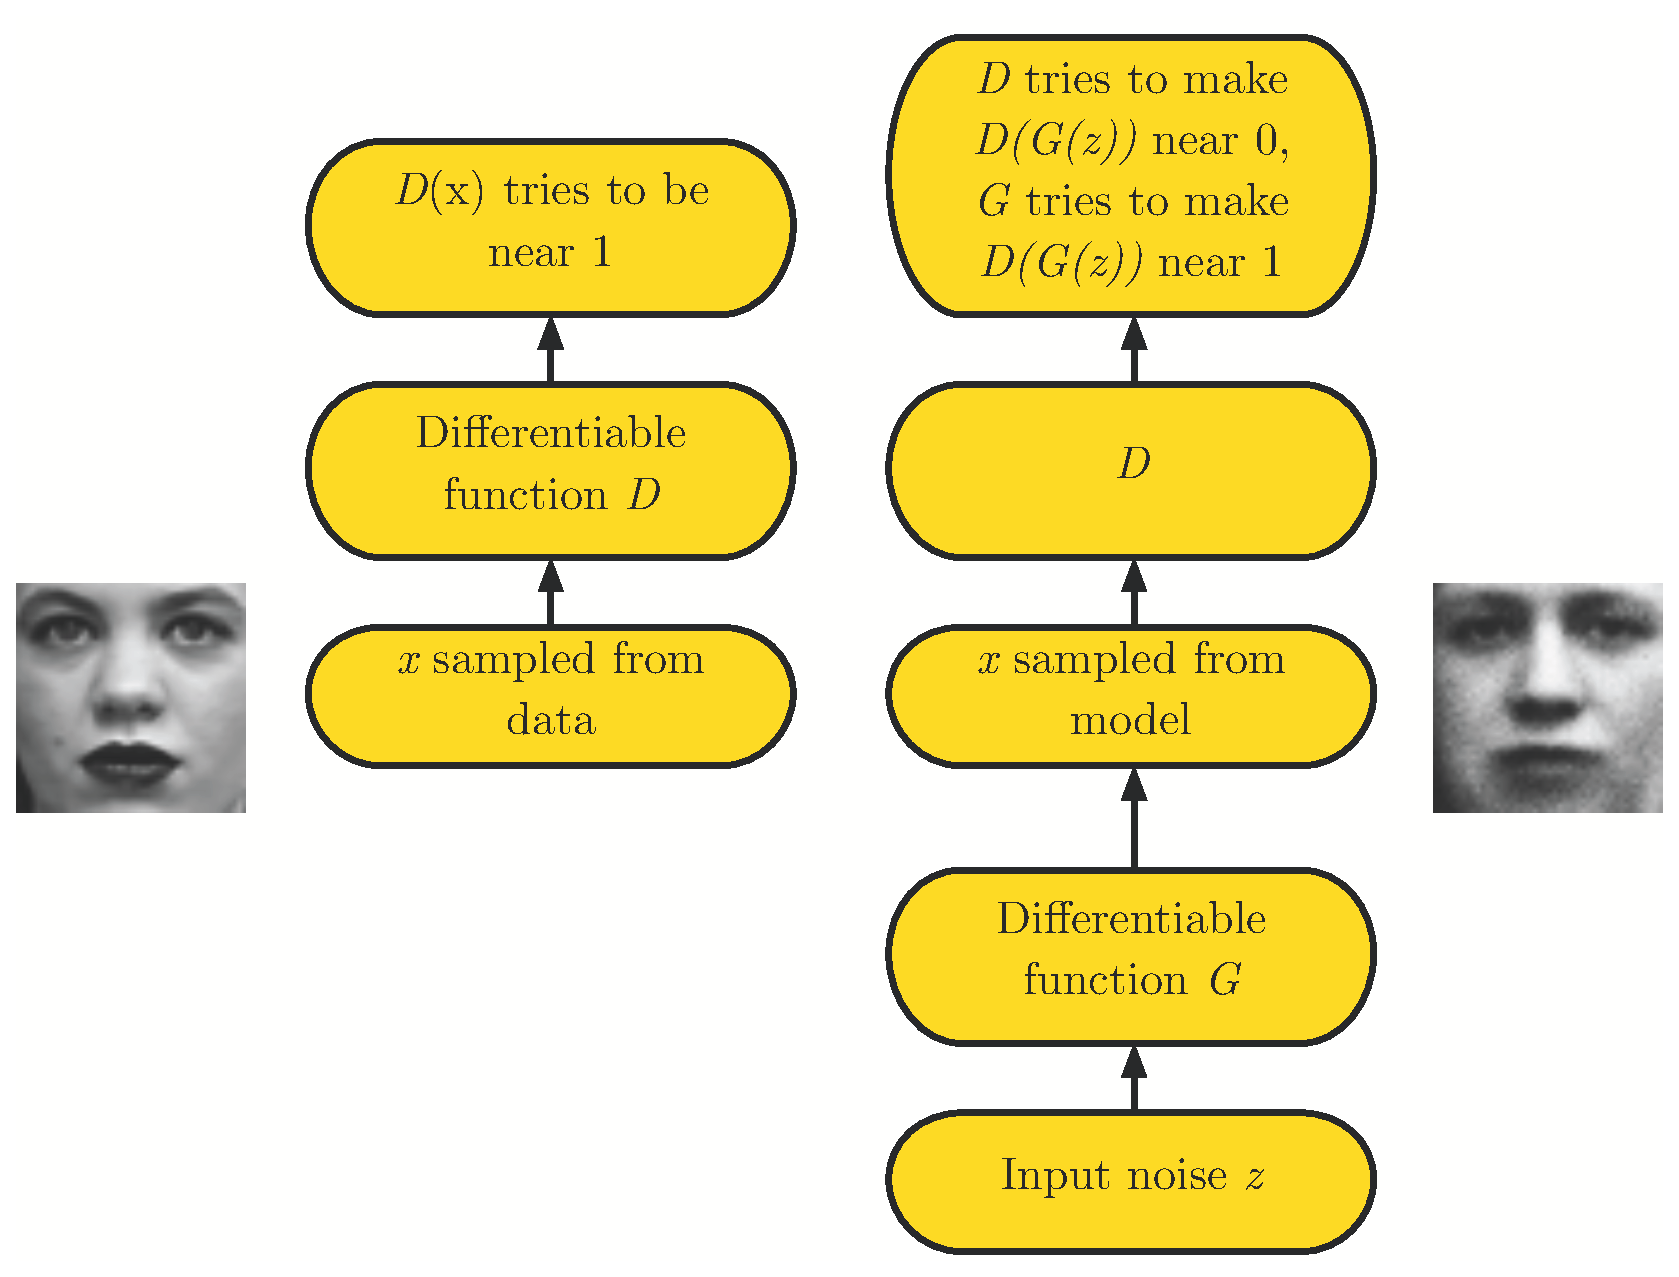
\includegraphics[width = 0.6\textwidth]{GAN_Framework}
 \end{figure}


由此我们可以得到GAN的优化目标如下,对模型$D$而言:
\begin{displaymath}
\mathbf{J}^{D}=-\frac{1}{2}\mathbb{E}_{{x}\sim p_{data}}\log{D({x})}-\frac{1}{2}\mathbb{E}_{{z}}\log(1-D(G({z}))))
\end{displaymath}
即,我们希望我们的模型$D$能够对数据集中所有的样本标记为1的概率最大,并对模型$G$产生的样本标记为0的概率最大。对模型$G$我们的优化目标正好同$D$相反,我们希望$G$产生的样本能够尽可能的让$D$标记为1,故而:
\begin{displaymath}
\mathbf{J}^{G}=\frac{1}{2}\mathbb{E}_{{z}}\log{(1-D(G({z})))}
\end{displaymath}

根据$\mathbf{J}^{D}$,我们求解$D(x)$如下:
\begin{displaymath}
\begin{split}
&\frac{\delta \mathbf{J}^{D}}{\delta D(x)} = \frac{\delta (-\frac{1}{2}\mathbb{E}_{{x}\sim p_{data}}\log{D({x})}-\frac{1}{2}\mathbb{E}_{{z}}\log(1-D(G({z}))))}{\delta D(x)} =0\\
&\mathbb{E}_{{x}\sim p_{data}}\log{D({x})} = \sum_{x}{p_{data}(x)\log{D(x)}}\\
&\mathbb{E}_{z}\log{(1-D(G(z)))} = \sum_{x}{p_{model}(x)\log{(1-D(x))}}\\
&\sum_{x}{\frac{p_{data}(x)}{D(x)} - \frac{p_{model}(x)}{1-D(x)}} = 0\\
&D(x) = \frac{p_{data}(x)}{p_{data}(x) + p_{model}(x)}\\
\end{split}
\end{displaymath}

GAN的训练算法如下:

\begin{figure}[htbp]
\centering
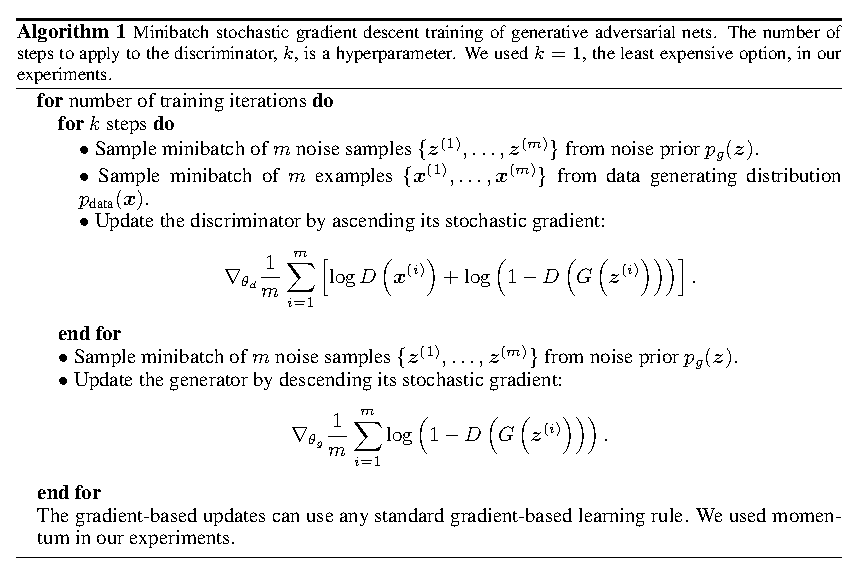
\includegraphics[width = 0.9\textwidth]{GAN_Train}
\end{figure}


下图是训练过程的一个形象化的演示:黑色虚线表示了数据的真实分布$\hat{G}$(未知的,我们只知道数据本身),绿色实线表示初始的$G$,蓝色虚线表示初始的$D$。初始的$G$同数据的真实分布$\hat{G}$差别较大,并不能很好的拟合数据,而初始的$D$也不能对一个样本是来自数据还是来自$G$做出很好的判别。我们固定$G$来训练$D$之后,$D$能够对区分$\hat{G}$和$G$,我们进一步的固定$D$来训练$G$使得$G$更接近$\hat{G}$,从而迷惑$D$。重复这个过程之后$G$将会尽可能的接近$\hat{G}$,而$D$会不能区分$G$和$\hat{G}$。
\begin{figure}[htbp]
\centering
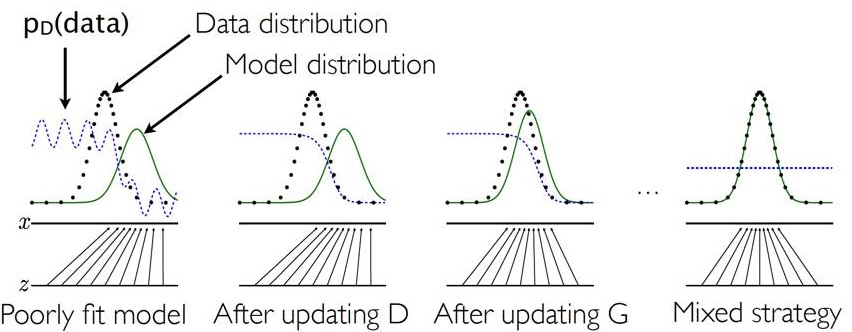
\includegraphics[width = 1.0\textwidth]{GAN_UpdateDG}
\end{figure}

令$P_r$为真实数据的分布,$P_g$为生成器的数据分布,则生成器的算是可以写为:$\mathbb{E}_{x \sim P_g}[\log (1- D(x))]$。我们将该损失添加一个不依赖于生成器的一项,变为:$\mathbb{E}_{x \sim P_r}[\log (D(x))] + \mathbb{E}_{x \sim P_g}[\log (1- D(x))]$,并将$D(x) = \frac{P_{r}(x)}{P_{r}(x) + P_{g}(x)}$带入得:

\begin{displaymath}
\begin{split}
&\mathbb{E}_{x \sim P_r}[\log (D(x))] + \mathbb{E}_{x \sim P_g}[\log (1- D(x))] \\
&= \mathbb{E}_{x \sim P_r}[\log (\frac{P_{r}(x)}{P_{r}(x) + P_{g}(x)})] + \mathbb{E}_{x \sim P_g}[\log (1- \frac{P_{r}(x)}{P_{r}(x) + P_{g}(x)})] \\
&= \mathbb{E}_{x \sim P_r}[\log (\frac{P_{r}(x)}{P_{r}(x) + P_{g}(x)})] + \mathbb{E}_{x \sim P_g}[\log (\frac{P_{g}(x)}{P_{r}(x) + P_{g}(x)})] \\
&= \mathbb{E}_{x \sim P_r}[\log (\frac{P_{r}(x)}{\frac{1}{2}(P_{r}(x) + P_{g}(x))})] + \mathbb{E}_{x \sim P_g}[\log (\frac{P_{g}(x)}{\frac{1}{2}(P_{r}(x) + P_{g}(x))})] -2 \log 2 \\
&= 2 JS(P_r, P_g) - 2log2\\
\end{split}
\end{displaymath}

即生成器的训练实际上是最小化真是数据分布$P_r$和模型数据分布$P_g$的JS距离。

\section{非饱和GAN}
当我们使用:$\mathbb{E}_{x \sim P_g}[\log (1- D(x))]$作为生成器的损失时会存在一个问题,就是在训练G时,我们最小化$JS(P_r, P_g)$,而在训练D时,我们最大化$JS(P_r, P_g)$。当判别器D以非常高的置信度拒绝一个样本时,产生器G的梯度就会消失。为了解决这个问题,我们可以将产生器的损失变换为$-\mathbb{E}_{x \sim P_g}[\log (D(x))]$。

\begin{displaymath}
\begin{split}
KL(P_g \parallel P_r) &= \mathbb{E}_{x \sim P_g} [\log \frac{P_g(x)}{P_r(x)}]\\
&= \mathbb{E}_{x \sim P_g} [\log \frac{P_g(x)/(P_r(x) + P_g(x))}{P_r(x)/(P_r(x) + P_g(x))}]\\
&= \mathbb{E}_{x \sim P_g} [\log \frac{1-D(x)}{D(x)}]\\
&= \mathbb{E}_{x \sim P_g} [\log {1-D(x)}] -\mathbb{E}_{x \sim P_g} [\log {D(x)}]\\
\mathbb{E}_{x \sim P_r}[\log (D(x))] + \mathbb{E}_{x \sim P_g}[\log (1- D(x))] &= 2 JS(P_r, P_g) - 2log2\\
-\mathbb{E}_{x \sim P_g}[\log (D(x))] &= KL(P_g \parallel P_r) - 2 JS(P_r, P_g) + 2log2 + \mathbb{E}_{x \sim P_r} [\log {D(x)}]\\
\end{split}
\end{displaymath}

则训练产生器G的优化目标$-\mathbb{E}_{x \sim P_g}[\log (D(x))]$,转换为$KL(P_g \parallel P_r) - 2 JS(P_r, P_g)$(公式中最后两项与G无关)。这样的一个优化目标是有问题的,它同时要求最小化$P_g$和$P_r$的KL距离,而又最大化两者的JS距离,在数值上会导致梯度非常的不稳定。另一方面由于KL距离是一个非对称的距离,这会导致
\begin{itemize}
\item 当$P_g(x) \to 0$而$P_r(x) \to 1$时,KL距离为0,
\item 当$P_g(x) \to 1$而$P_r(x) \to 0$时,KL距离为无穷大,
\end{itemize}
也就是说,当生成器没能够生成真实样本时,惩罚比较小,但当生成器生成了一个不真实的样本时,惩罚非常大。这样子训练出来的模型就会宁愿多生成一个重复而保险的样本,也不会冒险生成多样性的样本,这就是mode collapse问题。

\section{WGAN}
\subsection{不同的距离函数}
令 $\mathcal{X}$为紧矩阵空间(比如$[0,1]^d$),$\Sigma$为该空间的所有Borel子集的集合,$Prob(\mathcal{X})$为定义在$\mathcal{X}$上的概率分布的空间,对于任意的两个概率分布$\mathbb{P}_r, \mathbb{P}_g \in Prob(\mathcal{X})$,我们可以有如下的几个距离函数:

\textbf{Total Variantion(TV) Distance}: $\delta{({P}_r, {P}_g)} = \underset{A \in \Sigma}{sup} \left | {P}_r(A) -{P}_g(A) \right |$。 TV距离试图在定义域$\mathcal{X}$上寻找一个子集$A$,使得在该子集上两个概率分布的差最大。该最大的差即为TV距离。

\textbf{Kullback-Leibler(KL) Distance}: $KL({P}_r \parallel {P}_g) = \int \log (\frac{P_r(x)}{P_g(x)})P_r(x) \mathrm{d} \mu(x) $,其中$\mu(x)$为定义在$\mathcal{X}$上的测度。KL距离是非对称的,并且当$P_g{x} = 0$并且$P_r(x) > 0$时,其距离为无穷大。

\textbf{Jensen-Shannon(JS) Distance}:$JS({P}_r, {P}_g) = \frac{1}{2}KL({P}_r \parallel {P}_m) + \frac{1}{2}KL({P}_g \parallel {P}_m)$,其中${P}_m = \frac{\mathbb{P}_r + \mathbb{P}_g}{2}$。JS距离是对称的,{\color{red} 如果其中的$KL$距离的$\mu = \mathbb{P}_m$,则JS距离则在空间$\mathcal{X}$上永远有定义}。

\textbf{Earth Mover(EM) Distance}:$W({P}_r,{P}_g) = \underset{\gamma \in \Pi({P}_r, {P}_g)}{inf} \mathbb{E}_{(x,y) \sim \gamma} [\left \| x-y \right \|]$. 其中,$\gamma(x,y)$是以 $\mathbb{P}_r(x)$和$\mathbb{P}_g(x)$为边缘分布的$(x,y)$的联合分布, $\Pi({P}_r, {P}_g)$为所有$\gamma$的集合。对于一个可能的联合分布$\gamma$,我们可以采样一个$(x,y)$,并计算其距离$\left \| x-y \right \|$。对于分布$\gamma$,我们便可以计算在该分布下,距离$\left \| x-y \right \|$的期望值。在所有的可能的联合分布$\gamma$中,我们可以找到一个分布使得该距离的期望最小,这个最小的期望,便是EM距离。直觉上,如果我们把$\mathbb{P}_r$和$\mathbb{P}_g$看作在定义域上两种不同方式堆积的土堆,并$\gamma(x,y)$定义了如何将土堆${P}_r$变为${P}_g$的移动方式,那么EM距离就是将${P}_r$转变为${P}_g$的所有需要移动的单位小块的最小距离之和。

\textbf{平行线例子}: 我们令$Z \sim U[0,1]$,并令${P}_0$为$(0, Z) \in {R}^2$的分布,该分布在x轴上只在点0处有密度,而在y轴上在$[0,1]$区间上均匀分布。类似的,我们令${P}_\theta$为$(\theta, Z) \in \mathbb{R}^2$的分布,该分布在x轴上只在点$\theta$处有密度,而在y轴上在$[0,1]$区间上均匀布分布。那么分布${P}_0$和分布${P}_\theta$的距离为:
\begin{displaymath}
\begin{split}
\delta({P}_0, {P}_\theta) &= 
\begin{cases}  
1 ~~~ if ~~\theta \neq 0\\
0 ~~~ if ~~ \theta = 0\\
\end{cases}\\
KL({P}_0 \parallel {P}_\theta) &= KL({P}_\theta \parallel {P}_0) = 
\begin{cases}  
+ \infty ~~~ if ~~\theta \neq 0\\
0 ~~~ if ~~ \theta = 0\\
\end{cases}\\
JS({P}_0, {P}_\theta) &= 
\begin{cases}  
\log 2 ~~~ if ~~\theta \neq 0\\
0 ~~~ if ~~ \theta = 0\\
\end{cases}\\
W({P}_0, {P}_\theta) &= |\theta|\\
\end{split}
\end{displaymath}

对于TV距离,很明显,我们选定义域$\mathcal{X}$的一个子集$(0, [0,1])$, ${P}_0$在该子集上概率为1, ${P}_\theta$在该子集上概率为0,且其差为最大。

对于KL距离:
\begin{displaymath}
\begin{split}
KL({P}_0 \parallel {P}_\theta) &= \int_{0}^{1} \log (\frac{P_0(0,x)}{P_\theta(0,x)})P_0(0,x) \mathrm{d} x + \int_{0}^{1} \log (\frac{P_0(\theta,x)}{P_\theta(\theta,x)})P_0(\theta,x) \mathrm{d} x
\end{split}
\end{displaymath}
很明显当$\theta =0$时,其值为0, 当$\theta \neq 0$时,在子空间$(0,[0,1])$上积分为$+\infty$,在子空间$(\theta, [0,1]$上积分为0,故,距离为$+\infty$。同样的$KL({P}_\theta \parallel {P}_0)$也是如此。

对JS距离, 当$\theta =0 $时,很明显距离为0, 当$\theta \neq 0$时,:
\begin{displaymath}
\begin{split}
2JS({P}_0 \parallel {P}_\theta) 
&= KL({P}_0 \parallel \frac{{P}_0 + {P}_\theta}{2}) + KL({P}_\theta \parallel \frac{{P}_0 + {P}_\theta}{2}) \\
&= \int_{0}^{1} \log (\frac{P_0(0,x)}{\frac{P_0(0,x) + P_\theta(0,x)}{2}})P_0(0,x) \mathrm{d} x +
   \int_{0}^{1} \log (\frac{P_0(\theta,x)}{\frac{P_0(\theta,x) + P_\theta(\theta,x)}{2}})P_0(\theta,x) \mathrm{d} x\\
&+ \int_{0}^{1} \log (\frac{P_\theta(0,x)}{\frac{P_0(0,x) + P_\theta(0,x)}{2}})P_\theta(0,x) \mathrm{d} x +
   \int_{0}^{1} \log (\frac{P_\theta(\theta,x)}{\frac{P_0(\theta,x) + P_\theta(\theta,x)}{2}})P_\theta(\theta,x) \mathrm{d} x\\
&= \int_{0}^{1} \log (\frac{P_0(0,x)}{\frac{P_0(0,x)}{2}})P_0(0,x) \mathrm{d} x +
   \int_{0}^{1} \log (\frac{0}{\frac{P_\theta(\theta,x)}{2}})*0 \mathrm{d} x\\
&+ \int_{0}^{1} \log (\frac{0}{\frac{P_0(0,x)}{2}}) *0 \mathrm{d} x +
   \int_{0}^{1} \log (\frac{P_\theta(\theta,x)}{\frac{P_\theta(\theta,x)}{2}})P_\theta(\theta,x) \mathrm{d} x\\
&=  \int_{0}^{1} \log (2)P_0(0,x) \mathrm{d} x + \int_{0}^{1} \log (2)P_\theta(\theta,x) \mathrm{d} x\\
&= 2 \log 2\\
JS({P}_0 \parallel {P}_\theta) &= \log 2\\
\end{split}
\end{displaymath}

对EM距离,我们选择以 ${P}_0(x)$和${P}_\theta(x)$为边缘分布的$(x,y)$的联合分布$\gamma(x,y)$为定义域为$(0, \theta, x, y)$上的分布,其中$x,y \in [0,1]$,则,在该分布下,距离的期望为:
\begin{displaymath}
\begin{split}
&\int_0^1 \int_0^1 p_{\gamma}(0,\theta,x, x) \left \| (0,x) - (\theta, x) \right \| \mathrm{d} x  \mathrm{d} y \\
&= \int_0^1 \int_0^1 p_{\gamma}(0,\theta,x, x)  \left \| (0,x) - (\theta, y) \right \| \mathrm{d} x   \mathrm{d} y\\
&= \int_0^1 \int_0^1 p_{\gamma}(0,\theta,x, x)  \sqrt {\theta ^ 2 + (x-y)^2}\mathrm{d} x \mathrm{d} y\\
& \leq \int_0^1 \int_0^1 p_{\gamma}(0,\theta,x, x) |\theta| \mathrm{d} x \mathrm{d} y\\
&= |\theta|\\
\end{split}
\end{displaymath}
不等式等号成立的条件是联合分布$\gamma(x,y)$为定义域为线段$(0, \theta, x, y=x)$上的均匀分布。

由上可知,当${P}_r$和${P}_g$没有重叠的时候,TV,KL, JS距离均为不连续函数,其导数为0。
更一般的,给定高维空间的两个分布${P}_r$和${P}_g$,当他们的支撑集是高维空间的低维流形时, ${P}_r$和${P}_g$重叠部分测度为0的概率为1。

对GAN的产生器来说,输入为一个低维的向量,产生一个高维的样本,其支撑集便是高维空间的低维流形。故而,GAN的产生器${P}_g$和真实分布${P}_r$几乎没有重叠的可能。故而当使用TV/KL/JS距离作为损失时,导数为0。

\subsection{WGAN}

由前边我们知道EM距离相比TV, KL, JS更适合来做GAN的loss function。然而当我们试图使用EM距离来取代KL/JS距离时,存在一个问题,因为EM距离里边需要计算所有可能联合分布的一个下界。$W({P}_r,{P}_g) = \underset{\gamma \in \Pi({P}_r, {P}_g)}{inf} \mathbb{E}_{(x,y) \sim \gamma} [\left \| x-y \right \|]$。我们可以使用Kantorovich-Rubinstein duality来将EM距离改写为:

\begin{displaymath}
\begin{split}
W({P}_r, {P}_g) & = \underset{\left \| f \right \|_{L} \leq 1}{sup} \mathbb{E} _{X \sim {P}_r}[f(x)] - \mathbb{E}_{x \sim {P}_g}[f(x)]
\end{split}
\end{displaymath}
其中 $ \underset{\left \| f \right \|_{L} \leq 1}{sup} $表示在所有的符合1-Lipschitz连续的函数中,寻找一个令$\mathbb{E} _{X \sim {P}_r}[f(x)] - \mathbb{E}_{x \sim {P}_g}[f(x)]$最大的上界。

那么什么是Lipschitz连续? Lipschitz连续是一个比连续更强的光滑性的条件。Lipschitz连续函数限制了函数改变的速度,函数的斜率必须小于一个Lipschitz常数的实数。设$d_X$和$d_Y$分别为$X$和$Y$空间的两个度量,函数$f:X \to Y$是K-Lipschitz连续的当且仅当对于任意的$x_1, x_2 \in X$, 有 $d_Y(f(x_1), f(x_2)) \leq K d_X(x_1, x_2)$。

我们进一步的将所有满足1-Lipschitz连续的函数约束在一个以$w \in \mathcal{W}$($\mathcal{W}$为参数空间)为参数的函数$f_w$的子空间里,则:

\begin{displaymath}
\begin{split}
W({P}_r, {P}_g) & = \underset{\left \| f \right \|_{L} \leq 1}{sup} \mathbb{E} _{X \sim {P}_r}[f(x)] - \mathbb{E}_{x \sim {P}_g}[f(x)]\\
& \ge \underset{w \in \mathcal{W}}{max} \mathbb{E} _{X \sim {P}_r}[f_w(x)] - \mathbb{E}_{x \sim {P}_g}[f_w(x)]\\
\end{split}
\end{displaymath}

当我们需要训练一个$P_g = g_\theta(Z)$来拟合$P_r$时,我们首先要训练一个$f_w$来计算EM距离,然后基于这个EM距离来优化$g_\theta$,具体的:
\begin{itemize}
\item 给定$\theta$,训练$f_w$收敛以获得EM距离 $W(P_r, P_g)$的一个近似。
\item 给定优化的$f_w$,采样若干的$z \sim Z$,并计算$\theta$的梯度:$\nabla_\theta W(P_r, P_g) = \nabla_\theta(\mathbb{E}_{x \sim P_r}[f_w(x)] - \mathbb{E}_{z \sim Z}[f_w(g_\theta(z))]) = -\mathbb{E}_{z \sim Z}[f_w(g_\theta(z))]) $.
\item 更新$\theta$,并重复步骤1.
\end{itemize} 

具体的WGAN的训练过程为:

 \begin{figure}[htbp]
 \centering
 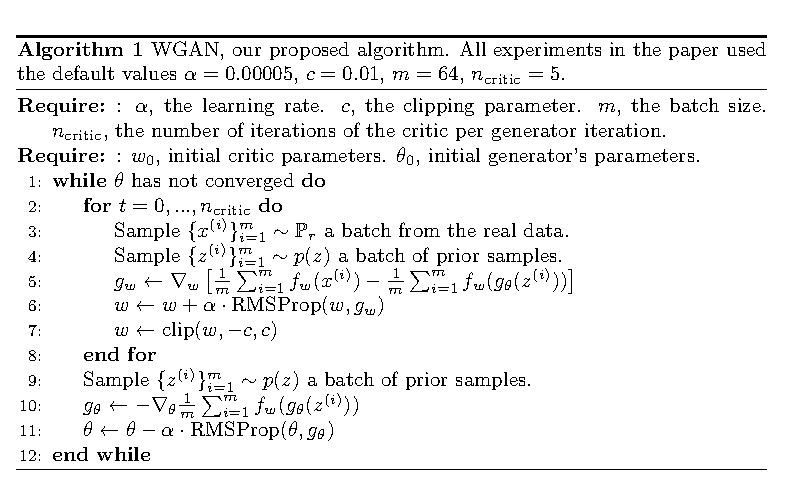
\includegraphics[width = 0.9\textwidth]{WGAN}
 \end{figure}

同原始的GAN相比,WGAN有如下几点改动:
\begin{itemize}
\item 判别器最后一层去调sigmoid,即已经不能做分类,可以看作一个critic
\item 生成器和判别器的loss不取log,因为仅仅是一个Lipschitz连续的函数,已经不是概率,有可能为负。
\item 每次更新判别器的参数之后,绝对值要截断到不超过常数$c$,以保证更新完之后仍然是一个Lipschitz连续的函数。
\item 不要使用基于动量的优化算法(Momentum和Adam),推荐RMSProp和SGD。 
\end{itemize} 


\section{DCGAN}

\section{SeqGAN}
% !Mode:: "TeX:UTF-8"

\chapter{VAE}

% !Mode:: "TeX:UTF-8"

\chapter{Reparameterization Trick}

\section{为什么需要Reparameterization}
当我们需要优化的系统中有一个从某个分布采样得到的样本作为另一个函数的输入,这个不确定的采样得到的样本使得梯度回传存在问题, 如图:
\begin{figure}[htbp]
\centering
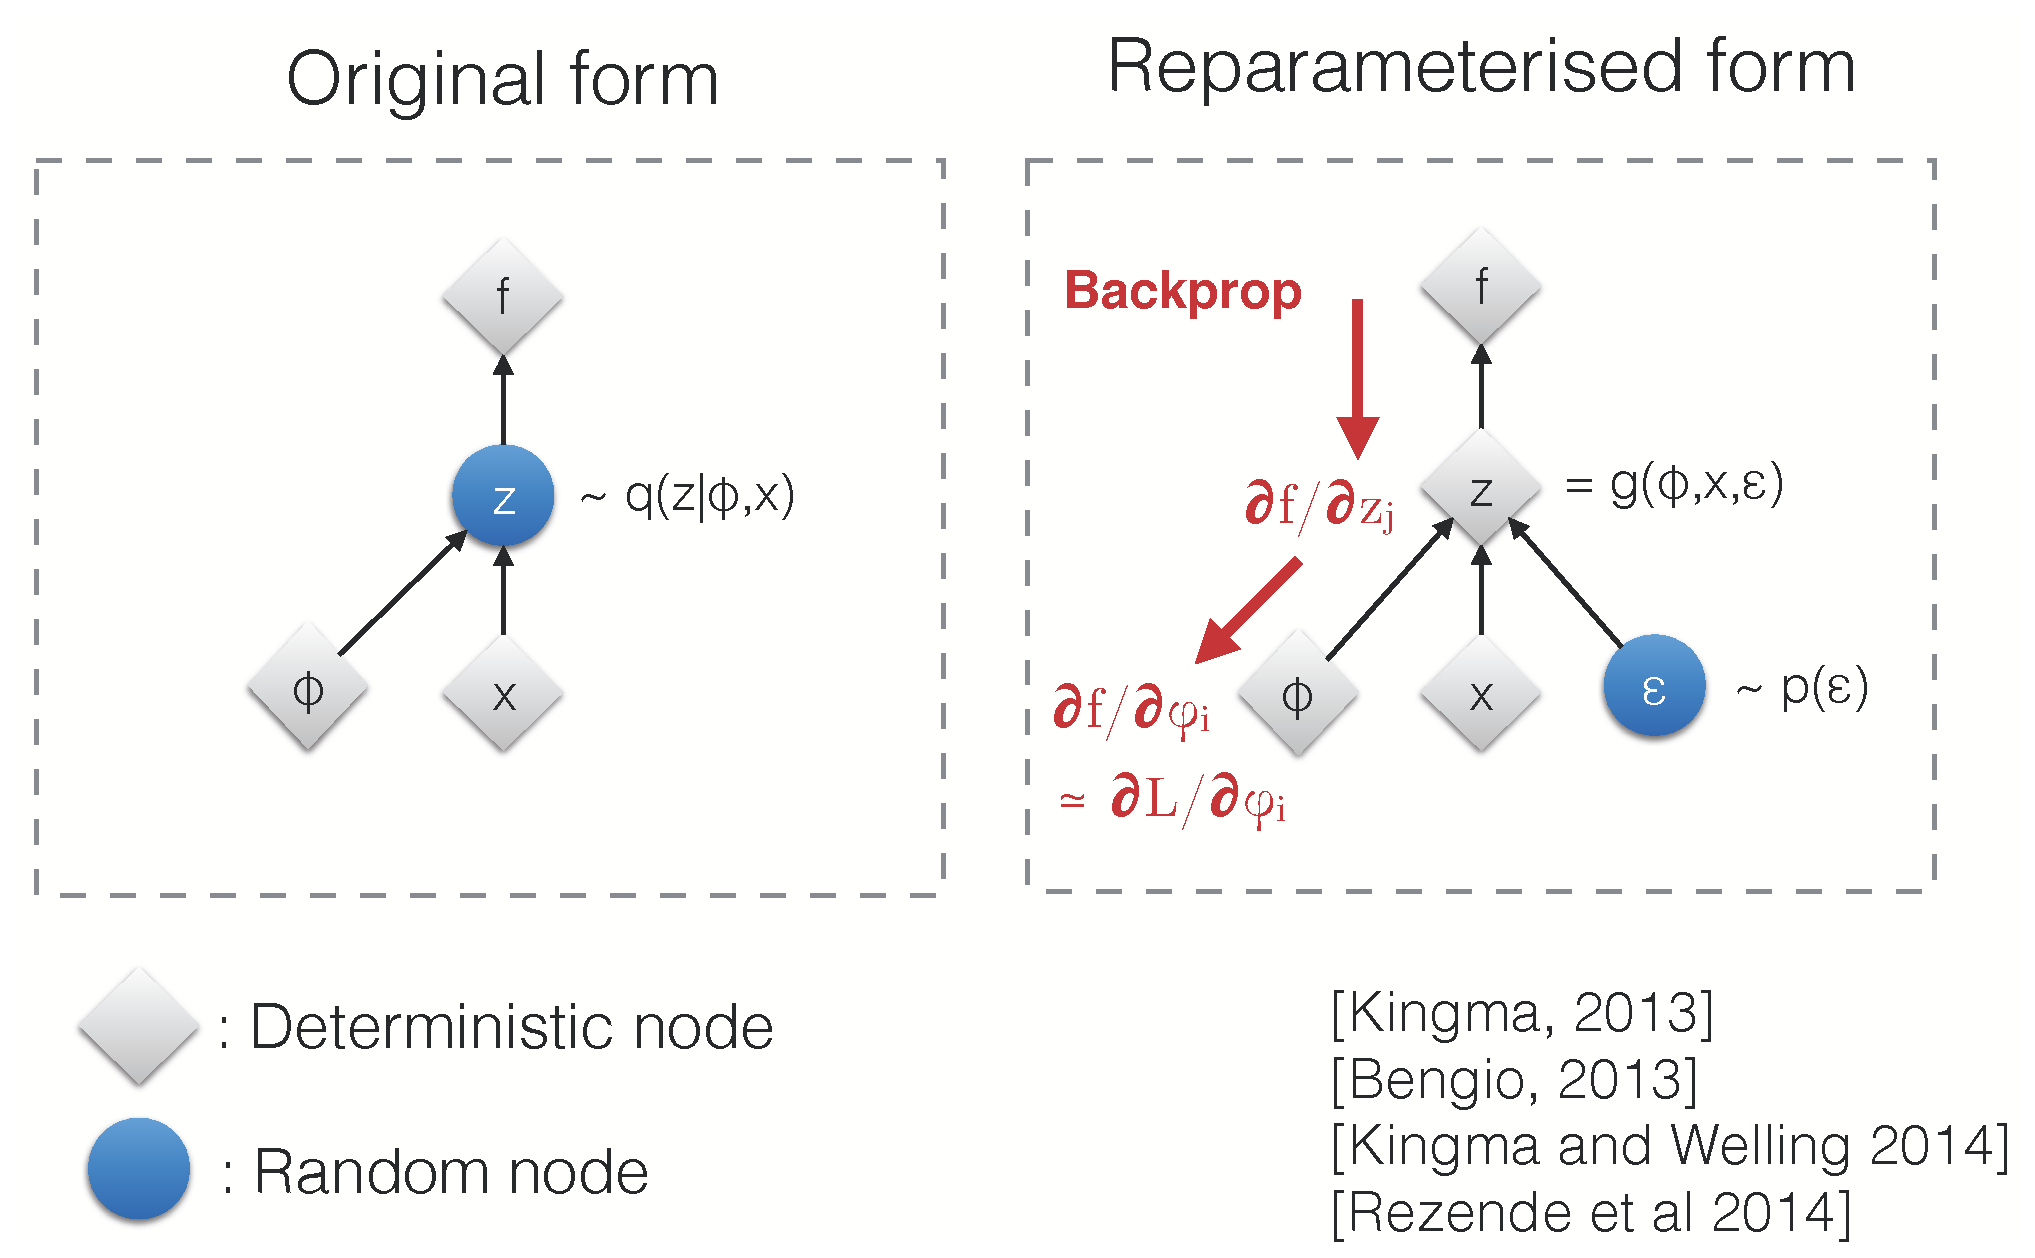
\includegraphics[width = 0.6\textwidth]{Reparameterization}
\end{figure}

假设$z$是服从以$\phi$和$x$为参数的分布$p(x|\phi, x)$,从该分布采样得到的$z$作为函数$f$的输入。由于$z$是采样得到的,故而不是确定的。所以在求导运算中便无法通过链式法则得到$\phi$和$x$的导数。reparameterization的技巧是通过将非确定节点移到运算树的叶节点上,从而可以应用链式法则求导。具体的做法是首先通过一个采样过程得到一个非确定的值$\varepsilon$,然后将$\varepsilon$同原始的参数$\phi$和$x$进行某种运算$g(\phi, x, \varepsilon)$得到$z$。

\section{Gaussian Reparameterization}
 如下图,在Variational Autoencoder模型中,我们需要将输入$x$编码为一个均值为$\mu$,方差为$\Sigma$的高斯分布然后从该高斯分布中采样一个隐变量$z$作为解码器的输入,该解码器将重构原始输入$x$。编码器和解码器可以是任意类型的神经网络。由于$z$是采样得到的不确定变量,所以在神经网络的训练过程中便无法使用反向传播来将梯度传给编码器。Reparameterization方法将该过程转换为给定输入$x$,编码器负责生成参数$\mu$和$\Sigma$,我们从标准正态分布中采样一个noise $\varepsilon$,然后通过$z=\mu + \Sigma*\varepsilon$得到需要的$z$。即,$\varepsilon$服从标准正太分布,则$z=\mu + \Sigma*\varepsilon$服从均值为$\mu$,方差为$\Sigma$的正太分布。令$F$为$z$的分布函数,则证明如下:
\begin{displaymath}
\begin{split}
F_z(x)&=P(z \leq x) = P(\mu + \Sigma*\varepsilon \leq x)=P(\varepsilon \leq \frac{x-\mu}{\Sigma}) = F_{\varepsilon}(\frac{x-\mu}{\Sigma})\\
f_Z(x) &= \frac{f_{\varepsilon}(\frac{x-\mu}{\Sigma})}{\Sigma} =\frac{1}{\sqrt{2\pi}\Sigma} exp \left\{ -\frac{(x-\mu)^2}{2 \Sigma^2} \right\} 
\end{split}
\end{displaymath}

\begin{figure}[htbp]
\centering
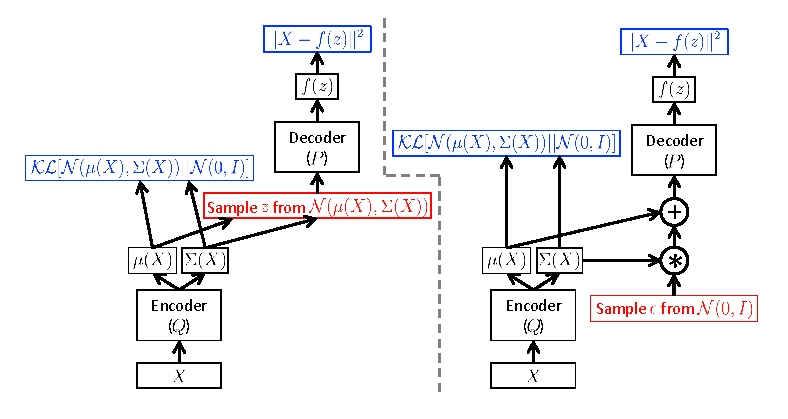
\includegraphics[width = 0.8\textwidth]{Vae_Reparameter}
\end{figure}

\section{Gumbel Max}

Gumbel Dsitribution 是定义在$(-\infty, +\infty)$之间的一个分布函数,定义如下:
\begin{displaymath}
p(x)=e^{-(x-\mu)-e^{-(x-\mu)}}
\end{displaymath}
其中$\mu$为一个均值参数,可以证明$p(x)$为一个概率分布。首先显然$e^{-(x-\mu)-e^{-(x-\mu)}}>0$,我们证明其和为1:

\begin{displaymath}
\begin{split}
\int_{-\infty}^{+\infty}p(x)\,\mathrm{d}x &=\int_{-\infty}^{+\infty}e^{-(x-\mu)-e^{-(x-\mu)}}\,\mathrm{d}x\\
&=\int_{-\infty}^{+\infty}e^{-x-e^{-x}}\,\mathrm{d}x\\
&\text{let } u=e^{-x}, \mathrm{d}u=-e^{-x}\mathrm{d}x=-u\mathrm{d}x\\
&=\int_{+\infty}^{0}-\frac{e^{\log{u}-e^{\log{u}}}}{u}\mathrm{d}u\\
&=\int_{+\infty}^{0}-e^{-u}\mathrm{d}u\\
&=\int_{0}^{+\infty}e^{u}\mathrm{d}u\\
&=1
\end{split}
\end{displaymath}

从而该分布的累计分布函数为: 
\begin{displaymath}
p(X \leqq x)=\int_{-\infty}^{x}e^{-(t-\mu)-e^{-(t-\mu)}}\mathrm{d}t =e^{-e^{-(x-\mu)}}
\end{displaymath}

在做多分类问题时,softmax通常被用来将多维的实数$[a_0, a_1, ... ,a_n]$映射为同样维度的概率分布$[p_0, p_1, ..., p_n]$, 其定义如下:
\begin{displaymath}
p(x)=\frac{e^{a_x}}{\sum_k{e^{a_k}}}
\end{displaymath}
有了这个$n$维的分布,我们便可以从该分布上采样。Gumbel Max则是用来将采样问题转化为一个优化问题。具体的,对于给定的一个softmax的分布,我们可以将每个$a_k$上加上一个$\mu=0$的Gumbel分布的noise,并取$argmax$,这样得到的最大值$k$遵从原来softmax的分布。

按此过程采样的结果为$x$,那么$x=k$的意思是对于$\forall k' \ne k, a_k + n_k \ge a_{k'} + n_{k'} $:
\begin{displaymath}
\begin{split}
p(x=k) &= \int ...\int{p(a_k + n_k \ge a_{k'} + n_{k'}, \forall k' \ne k)} \mathrm{d}n_1 ... \mathrm{d}n_K\\
&=\int p(n_k) \left[   \prod_{k' \neq k} \int p(a_k + n_k \ge a_{k'} + n_{k'}|n_k) \mathrm{d} n_{k}'  \right] \mathrm{d} n_k\\
&=\int p(n_k) \left[   \prod_{k' \neq k} \int p(n_{k'} \leq n_k + a_k - a_{k'}|n_k) \mathrm{d} n_{k}'  \right] \mathrm{d} n_k\\
&=\int p(n_k) \left[   \prod_{k' \neq k} e^{-e^{-(n_k+a_k-a_{k'})}}  \right] \mathrm{d} n_k\\
&=\int  e^{-n_k - e^{-n_k}} e^{-{\sum_{k \ne k'}{e^{-(n_k+a_k-a_{k'})}}}} \mathrm{d} n_k\\
&=\int  e^{-n_k - e^{-n_k}} e^{-e^{-n_k}(\sum_{k \ne k'}{e^{-(a_k-a_{k'})}})} \mathrm{d} n_k\\
&=\int  e^{-n_k - e^{-n_k}}e^{-e^{-n_k} (\sum_{k'}{e^{-(a_k-a_{k'})}})} \mathrm{d} n_k\\
\text{let } A &=\log \sum_{k'} e^{-(a_k-a_{k'})} = \log e^{-a_k} (\sum_{k'} e^{a_{k'}}) = \log{\sum_{k'} e^{a_{k'}}} -a_k:\\
&= \int e^{-n_k - e^{-n_k} - e^{-n_k  + A}} \mathrm{d} n_k\\
&=e^{-A} \int e^{-(n_k-A)-e^{-(n_k-A)}} \mathrm{d} n_k\\
&= e^{-A} = \frac{e^{a_k}}{\sum_{k'}{e^{a_{k'}}}}
\end{split}
\end{displaymath}





\end{CJK*}
\end{document}
